\RequirePackage{rotating}
\documentclass{article}

% Bibliography
\usepackage{natbib}
\bibpunct{(}{)}{;}{a}{}{;}

% Use 'It was found that A is B (Name 1234)' style
\setcitestyle{authoryear,open={},close={}}

% Affiliations
\usepackage{authblk}

% RJCB: I think this title is better: 
% (1) tree prior importantance is the goal, the error is just the means
% (2) no need to specify BEAST2, it's also just a means
\title{
  pirouette:
  Quantifying the importance of a tree prior in Bayesian phylogenetics
}
% \title{pirouette: Determining the error BEAST2 makes in inferring a phylogeny}

\author[1]{Rich\`el J.C. Bilderbeek}
\author[1]{Giovanni Laudanno}
\author[1]{Rampal S. Etienne}
\affil[1]{Groningen Institute for Evolutionary Life Sciences, University of 
Groningen, Groningen, The Netherlands}

% Use double spacing
\usepackage{setspace}
\doublespacing

\usepackage{listings}
\usepackage{hyperref}
\usepackage{todonotes}
\usepackage{verbatim}
\usepackage{pgf}
\usepackage{bm}
\usepackage{multirow}
\usepackage{amsfonts}
\usepackage{array}
\usepackage{array}
\usepackage{booktabs}
\newcolumntype{C}[1]{>{\centering\arraybackslash}p{#1}}
\newcolumntype{L}[1]{>{\raggedright\arraybackslash}p{#1}}
\usepackage{longtable}
\usepackage{rotating}
\usepackage{mathtools}

\usepackage{tkz-graph}
\usetikzlibrary{arrows,automata}
\usetikzlibrary{calc}
\usetikzlibrary{arrows.meta}

% sidewaysfigure
\usepackage{rotating}

% Style of listings
% From http://r.789695.n4.nabble.com/
%   How-to-nicely-display-R-code-with-the-LaTeX-package-listings-tp4648110.html
\usepackage{fancyvrb} 
\definecolor{codegreen}{rgb}{0,0.6,0}
\definecolor{codegray}{rgb}{0.5,0.5,0.5}
\definecolor{codepurple}{rgb}{0.58,0,0.82}
\definecolor{backcolor}{rgb}{0.95,0.95,0.92}
\lstdefinestyle{mystyle}{
  language=R,% set programming language
  basicstyle=\ttfamily\small,% basic font style
  commentstyle=\color{gray},% comment style
  % numbers=left,% display line numbers on the left side
  numberstyle=\scriptsize,% use small line numbers
  numbersep=10pt,% space between line numbers and code
  tabsize=2,% sizes of tabs
  showstringspaces=false,
  captionpos=b,% positioning of the caption below
  breaklines=true,% automatic line breaking
  escapeinside={(*}{*)},% escaping to LaTeX
  fancyvrb=true,% verbatim code is typset by listings
  extendedchars=false,% prohibit extended chars (chars of codes 128--255)
  alsoletter={.<-},% becomes a letter
  alsoother={$},% becomes other
  otherkeywords={!=, ~, $, \&, \%/\%, \%*\%, \%\%, <-, <<-, /},% other keywords
  deletekeywords={c}% remove keywords 
}
\lstset{style=mystyle}

% Adds numbered lines
\usepackage{lineno}
\linenumbers

% Rename 'Abstract' to 'Summary 
\usepackage[english]{babel}
\addto{\captionsenglish}{\renewcommand{\abstractname}{Summary}}

%comments
\newcommand{\giovanni}[1]{\textcolor{blue}{\textbf{[GL: #1]}}}
\newcommand{\richel}[1]{\textcolor{orange}{\textbf{[RB: #1]}}}
\newcommand{\rampal}[1]{\textcolor{green}{\textbf{[RSE: #1]}}}


\begin{document}

\maketitle

\begin{abstract}

  \textbf{1. }
    BEAST2 is a popular Bayesian phylogenetics software tool,
    that takes an alignment of characters (usually nucleotides) 
    and an inference model to create a
    posterior of jointly-estimated phylogenies and model parameters. 
    An important ingredient of BEAST2 is the species tree prior, 
    due to which the tool can be used for inference of 
    macroevolutionary processes underlying the species tree. 
    However, only models that allow for fast computation of 
    the prior probability are possible in practice. 
    This begs the question of how accurate the tree estimation is 
    when the real macroevolutionary processes are different 
    from those assumed in BEAST2. \\
  \textbf{2. }
    Here we present \verb;pirouette;, 
    a free, libre and open-source R package that assesses 
    the inference error BEAST2 makes based on a 
    phylogeny from any macroevolutionary diversification model. \\
  \textbf{3. }
    We describe \verb;pirouette;'s usage and the biological scientific
    question it can answer, including full examples. \\
  \textbf{4. }
    Last, we discuss the results obtained by the examples. \\
\end{abstract}

{\bf Keywords:} computational biology, evolution, phylogenetics, tree prior,
  Bayesian model selection, BEAST2, babette, pirouette, R

%%%%%%%%%%%%%%%%%%%%%%%%%%%%%%%%%%%%%%%%%%%%%%%%%%%%%%%%%%%%%%%%%%%%%%%%%%%%%%%%
\section{Introduction}
%%%%%%%%%%%%%%%%%%%%%%%%%%%%%%%%%%%%%%%%%%%%%%%%%%%%%%%%%%%%%%%%%%%%%%%%%%%%%%%%

The development of new powerful inference tools, 
such as BEAST [\cite{drummond2007beast}], 
MrBayes [\cite{huelsenbeck2001mrbayes}]
or RevBayes [\cite{hohna2016revbayes}], 
allows to build phylogenetic trees 
from character data (usually nucleotide sequences) extracted 
from extant (but also extinct) organisms.
This has constituted an important step forward 
in our understanding of how species evolve.
Such tools have been increasingly exploited to hypothesize 
and test what the main drivers and modes for diversification are.

BEAST [\cite{drummond2007beast}] is a Bayesian phylogenetics tool, 
that needs both data and priors to infer a posterior.
Of these priors, the tree prior describes how diversification occurs.
BEAST has built-in tree priors such as the Yule [\cite{yule}] and 
(constant-rate) birth-death [\cite{nee1994reconstructed}] model.
These simple tree priors are most commonly used, as these 
have sufficient biological complexity, while being computationally fast.
BEAST's successor, BEAST2 [\cite{bouckaert2014beast}],
has a package manager, that allows third-party users to extend existing 
functionality.
By writing a BEAST2 package, novel diversification models can be added.
The key ingredient of such a package would be the likelihood equation
of a phylogeny for the novel diversification model.
There have been plenty of these models (and their associated probability 
algorithms) 
developed, among others, those in which diversification is 
time-dependent [\cite{nee1994reconstructed}, \cite{rabosky2008explosive}], 
or diversity-dependent [\cite{etienne2011diversity}],
or that can shift [\cite{etienne2012conceptual}, 
\cite{rabosky2014automatic}, \cite{alfaro2009nine}, \cite{laudanno2018sls}].
Other birth-death models treat speciation as a process that takes 
time [\cite{rosindell2010protracted}][\cite{etienne2012prolonging}], 
or that happens in bursts of simultaneous 
events [\cite{laudanno2018mbd}], or that
depends on a trait that has two [\cite{maddison2007estimating}], 
or more [\cite{fitzjohn2012diversitree}] states,
or even allows concealed states [\cite{beaulieu2016detecting}] 
or a combination of all these [\cite{herrera2018detecting}].
Only few of these diversification models are available as a BEAST2 package.

When a novel diversification model is introduced,
its performance is commonly tested as well.
Part of a model's performance is its parameter 
recovery (e.g. [\cite{etienne2014estimating}]),
in which phylogenies are simulated from known parameters, 
after which the parameters are estimated from the phylogenies.
Ideally, the estimated parameter values closely match the known/true values.

Even when a diversification model passes the procedure described above,
it is not necessarily used in Bayesian inference.
In Bayesian inference, the likelihood of a diversification 
model, is computed millions of times.
Due to this, effective but computationally expensive tree priors are inviable.
Also, there may be no need to add such a tree prior to a Bayesian
inference framework: the more informative the data, 
the lower the influence the tree prior has.
Due to this, computionally faster tree priors are more commonly used.
However, it is unknown if it is valid to assume that tree prior choice is 
of low importance.

\richel{
  I think this is a usefull paragraph, adding some depth to this paper,
  but it could use some rewording
}
There have been multiple attemps to investigate the importance of tree
prior choice. For example, recently Sarver et al., [\cite{sarver2019choice}] 
show that the choice of tree prior does not 
substantially affect phylogenetic inferences of diversification rates.
Also recently, Duchene et al. [\cite{duchene2018phylodynamic}] released
a BEAST2 package to assess how well posterior predictive simulations
recover a given tree when using the standard diversification models.
These investigations show how current diversification models compare
to one another, but these do not help assess the importance of a 
new tree prio. 

Here we introduce a method to quantify the importance of a novel tree prior.
The method starts with a phylogeny generated by the process of 
a (usually novel) tree prior.
Using the tree priors built-in into BEAST2, 
a Bayesian posterior is inferred.
The more similar the phylogenies in the posterior are to the original phylogeny,
the less important the novel tree prior has been.
Only impactful tree priors will be worth the effort and computational burden 
to use in a Bayesian framework.

This method is programmed as an R package called \verb;pirouette;.
\verb;pirouette; is built on \verb;babette; [\cite{bilderbeek2018babette}], 
which calls BEAST2 [\cite{bouckaert2014beast}]. 

%%%%%%%%%%%%%%%%%%%%%%%%%%%%%%%%%%%%%%%%%%%%%%%%%%%%%%%%%%%%%%%%%%%%%%%%%%%%%%%%
\section{Description}
%%%%%%%%%%%%%%%%%%%%%%%%%%%%%%%%%%%%%%%%%%%%%%%%%%%%%%%%%%%%%%%%%%%%%%%%%%%%%%%%

\verb;pirouette; is written in the R programming language (\cite{R}).
The goal of \verb;pirouette; is to quantify the importance of a tree
prior. It does so by measuring the inference error BEAST2
makes for a given reconstructed phylogeny, 
simulated under the mechanisms of a (usually novel) diversification model, 
which we will refer to as the 'generative tree prior', $\mathit{P}$. 
Such a study will typically construct phylogenies 
for different combinations of the diversification model's parameters, 
to assess under which scenarios the error made by BEAST2 cannot be neglected. 
Although a well-conducted theoretical study uses many replicates, 
this article only shows examples with one replicate, for the sake of clarity.

\verb;pirouette; is very flexible and allows the user 
to specify a big variety of custom settings. 
These settings can be grouped in macro-sections, 
according to how they operate in the pipeline. 
We summarize them in tables~\ref{tab:options} and~\ref{tab:definitions}.

Although many possible tests can be performed, 
we present here what we think are the five most important 
example research questions (ERQ) that \verb;pirouette; can answer. 
For these ERQs we will quantify the importance of a tree prior.

\begin{sidewaystable}
\centering
  \begin{tabular}{|@{}c|p{2.5cm}|p{9cm}|p{4.5cm}@{}|}
    \hline
    \centering
    %%%%%%%%%%%%%%%%%%%%%%%%%%%%%%%%%%%%%%%%%%%%%%%%%%%%%%%%%%%%%%%%%%%%%%%%%%%%
    \textbf{Symbol} & \textbf{Sub-argument} & \textbf{Description} & 
\textbf{Possible values} \\ 
    \hline
    %%%%%%%%%%%%%%%%%%%%%%%%%%%%%%%%%%%%%%%%%%%%%%%%%%%%%%%%%%%%%%%%%%%%%%%%%%%%
    $\mathit{t_{p}}$ & tree prior & Macroevolutionary speciation model 
      & Yule, BD, CBS, CCP, CEP \\
    %%%%%%%%%%%%%%%%%%%%%%%%%%%%%%%%%%%%%%%%%%%%%%%%%%%%%%%%%%%%%%%%%%%%%%%%%%%%
    $\mathit{c_{m}}$ & clock model & Clock for the DNA mutation rates 
      & strict, relaxed log-normal \\
    %%%%%%%%%%%%%%%%%%%%%%%%%%%%%%%%%%%%%%%%%%%%%%%%%%%%%%%%%%%%%%%%%%%%%%%%%%%%
    $\mathit{s_{m}}$ & site model & Nucleotide substitution model 
      & JC, HKY, TN93, GTR \\
    %%%%%%%%%%%%%%%%%%%%%%%%%%%%%%%%%%%%%%%%%%%%%%%%%%%%%%%%%%%%%%%%%%%%%%%%%%%%
    $\mathit{m_{r}}$ & mutation rate & Pace at which mutation occurs 
      & $m_{r} \in \mathbb{R}_{>0}$\\
    %%%%%%%%%%%%%%%%%%%%%%%%%%%%%%%%%%%%%%%%%%%%%%%%%%%%%%%%%%%%%%%%%%%%%%%%%%%%
    $\mathit{r_{s}}$ & root sequence & DNA sequence at the root of the tree 
      & any combination of a, c, g, t \\
    %%%%%%%%%%%%%%%%%%%%%%%%%%%%%%%%%%%%%%%%%%%%%%%%%%%%%%%%%%%%%%%%%%%%%%%%%%%%
    $\mathit{m_{p}}$ & MRCA prior & Prior knowledge of a most recent common 
      ancestor & see documentation \\
    %%%%%%%%%%%%%%%%%%%%%%%%%%%%%%%%%%%%%%%%%%%%%%%%%%%%%%%%%%%%%%%%%%%%%%%%%%%%
    $\mathit{m_{s}}$ & MCMC settings & Markov Chain Monte Carlo algorithm setup 
      & see documentation \\
    %%%%%%%%%%%%%%%%%%%%%%%%%%%%%%%%%%%%%%%%%%%%%%%%%%%%%%%%%%%%%%%%%%%%%%%%%%%%
    $\mathit{m_{t}}$ & model type & Criterion to select an inference model 
      & Generative, Candidate \\
    %%%%%%%%%%%%%%%%%%%%%%%%%%%%%%%%%%%%%%%%%%%%%%%%%%%%%%%%%%%%%%%%%%%%%%%%%%%%
    $\mathit{r_{i}}$ & run if & Condition under which an inference model is 
      used & Always, Best candidate\\
    %%%%%%%%%%%%%%%%%%%%%%%%%%%%%%%%%%%%%%%%%%%%%%%%%%%%%%%%%%%%%%%%%%%%%%%%%%%%
    $\mathit{e_{f}}$ & error function & Specifies how to measure the error 
      & nLTT, $|\gamma|$ \\
    %%%%%%%%%%%%%%%%%%%%%%%%%%%%%%%%%%%%%%%%%%%%%%%%%%%%%%%%%%%%%%%%%%%%%%%%%%%%
    $\mathit{\tau_{p}}$ & twin tree prior & Sets the tree prior for the twin 
tree 
      & Yule, BD \\
    %%%%%%%%%%%%%%%%%%%%%%%%%%%%%%%%%%%%%%%%%%%%%%%%%%%%%%%%%%%%%%%%%%%%%%%%%%%%
    \hline
  \end{tabular}
  \caption{
    Most important parameter options. 
    BD = birth death (\cite{nee1994reconstructed}), 
    CBS = coalescent Bayesian Skyline (\cite{drummond2005bayesian}), 
    CCP = coalescent constant-population, 
    CEP = coalescent exponential-population,
    JC = Jukes-Cantor 1969 (\cite{jukes1969evolution}), 
    HKY = Hasegawa, Kishino and  Yano (\cite{hasegawa1985dating}), 
    TN93 = \cite{tamura1993estimation}, 
    GTR = Generalised time-reversible model (\cite{tavare1986some}).
  }
  \label{tab:options}
\bigskip

  \begin{tabular}{|@{}c|p{4cm}|p{9cm}|p{3cm}@{}|}
    \hline
    \centering
    %%%%%%%%%%%%%%%%%%%%%%%%%%%%%%%%%%%%%%%%%%%%%%%%%%%%%%%%%%%%%%%%%%%%%%%%%%%%
    \textbf{Symbol} & \textbf{Macro-argument} & \textbf{Description} 
      & \textbf{Includes} \\
    \hline
    %%%%%%%%%%%%%%%%%%%%%%%%%%%%%%%%%%%%%%%%%%%%%%%%%%%%%%%%%%%%%%%%%%%%%%%%%%%%
    $\mathit{P}$ & Generative tree prior & Diversification model to generate 
      the 'true' tree & $\mathit{t_{p}}$ \\
    %%%%%%%%%%%%%%%%%%%%%%%%%%%%%%%%%%%%%%%%%%%%%%%%%%%%%%%%%%%%%%%%%%%%%%%%%%%%
    $\mathit{A}$ & Alignment model & Model used to simulate the 
      alignment ($\mathit{c_{m}}$ must be strict) 
      & $\mathit{c_{m}}, \mathit{s_{m}}, \mathit{m_{r}}, \mathit{r_{s}}$ \\
    %%%%%%%%%%%%%%%%%%%%%%%%%%%%%%%%%%%%%%%%%%%%%%%%%%%%%%%%%%%%%%%%%%%%%%%%%%%%
    $\mathit{G}$ & Generative model & The full setting to produce BEAST2 input 
      data & $\mathit{P}$, $\mathit{A}$ \\
    %%%%%%%%%%%%%%%%%%%%%%%%%%%%%%%%%%%%%%%%%%%%%%%%%%%%%%%%%%%%%%%%%%%%%%%%%%%%
    $\mathit{I}$ & Inference model & Phylogenetic inference model to run BEAST2 
      & $\mathit{c_{m}}, \mathit{s_{m}}, \mathit{t_{p}}, 
      \mathit{m_{p}}, \mathit{m_{s}}$ \\
    %%%%%%%%%%%%%%%%%%%%%%%%%%%%%%%%%%%%%%%%%%%%%%%%%%%%%%%%%%%%%%%%%%%%%%%%%%%%
    $\mathit{C}$ & Inference conditions & Conditions under which $\mathit{I}$ 
      is used in the inference & $\mathit{m_{t}}, \mathit{r_{i}}$\\
    %%%%%%%%%%%%%%%%%%%%%%%%%%%%%%%%%%%%%%%%%%%%%%%%%%%%%%%%%%%%%%%%%%%%%%%%%%%%
    $\mathit{X}$ & Experiment (candidate) 
      & Full setting for a Bayesian inference 
      & $\mathit{I},\mathit{C}$ \\
    %%%%%%%%%%%%%%%%%%%%%%%%%%%%%%%%%%%%%%%%%%%%%%%%%%%%%%%%%%%%%%%%%%%%%%%%%%%%
    $\mathit{X'}$ & Experiment (selected) & As above & 
      $\mathit{I},\mathit{C}$, $Pr(D)$, $\omega$ \\
    %%%%%%%%%%%%%%%%%%%%%%%%%%%%%%%%%%%%%%%%%%%%%%%%%%%%%%%%%%%%%%%%%%%%%%%%%%%%
    $\mathit{E}$ & Error measure parameters & Errors measurement setup & 
      $\mathit{e_{f}}$\\
    %%%%%%%%%%%%%%%%%%%%%%%%%%%%%%%%%%%%%%%%%%%%%%%%%%%%%%%%%%%%%%%%%%%%%%%%%%%%
    $\mathit{T}$ & Twinning parameters & Twin tree creation procedure & 
      $\mathit{\tau_{p}}$\\
    %%%%%%%%%%%%%%%%%%%%%%%%%%%%%%%%%%%%%%%%%%%%%%%%%%%%%%%%%%%%%%%%%%%%%%%%%%%%
    \hline 
  \end{tabular}
  \caption{
    Definitions of terms and relative symbols used in the main text and in 
    Fig~\ref{fig:pipeline}. $Pr(D)$ denotes the evidence, $\omega$ denotes
    a model's weight 
  }
  \label{tab:definitions}
  \giovanni{
    Should we rename "Twinning Parameters" to "Twinning model"?
  }
  \richel{
    As the twinning parameters contain more than only the twin model's tree 
    prior, I suggest to keep it 'twinning parameters'
  }
  \giovanni{I don't completely get the $X'$ description. What are $Pr(D)$ and 
$\omega$? Is it something that we really need or it brings more complications 
than benefits?}
\end{sidewaystable}

\subsection{pirouette's pipeline}

\begin{figure}
  \centering
  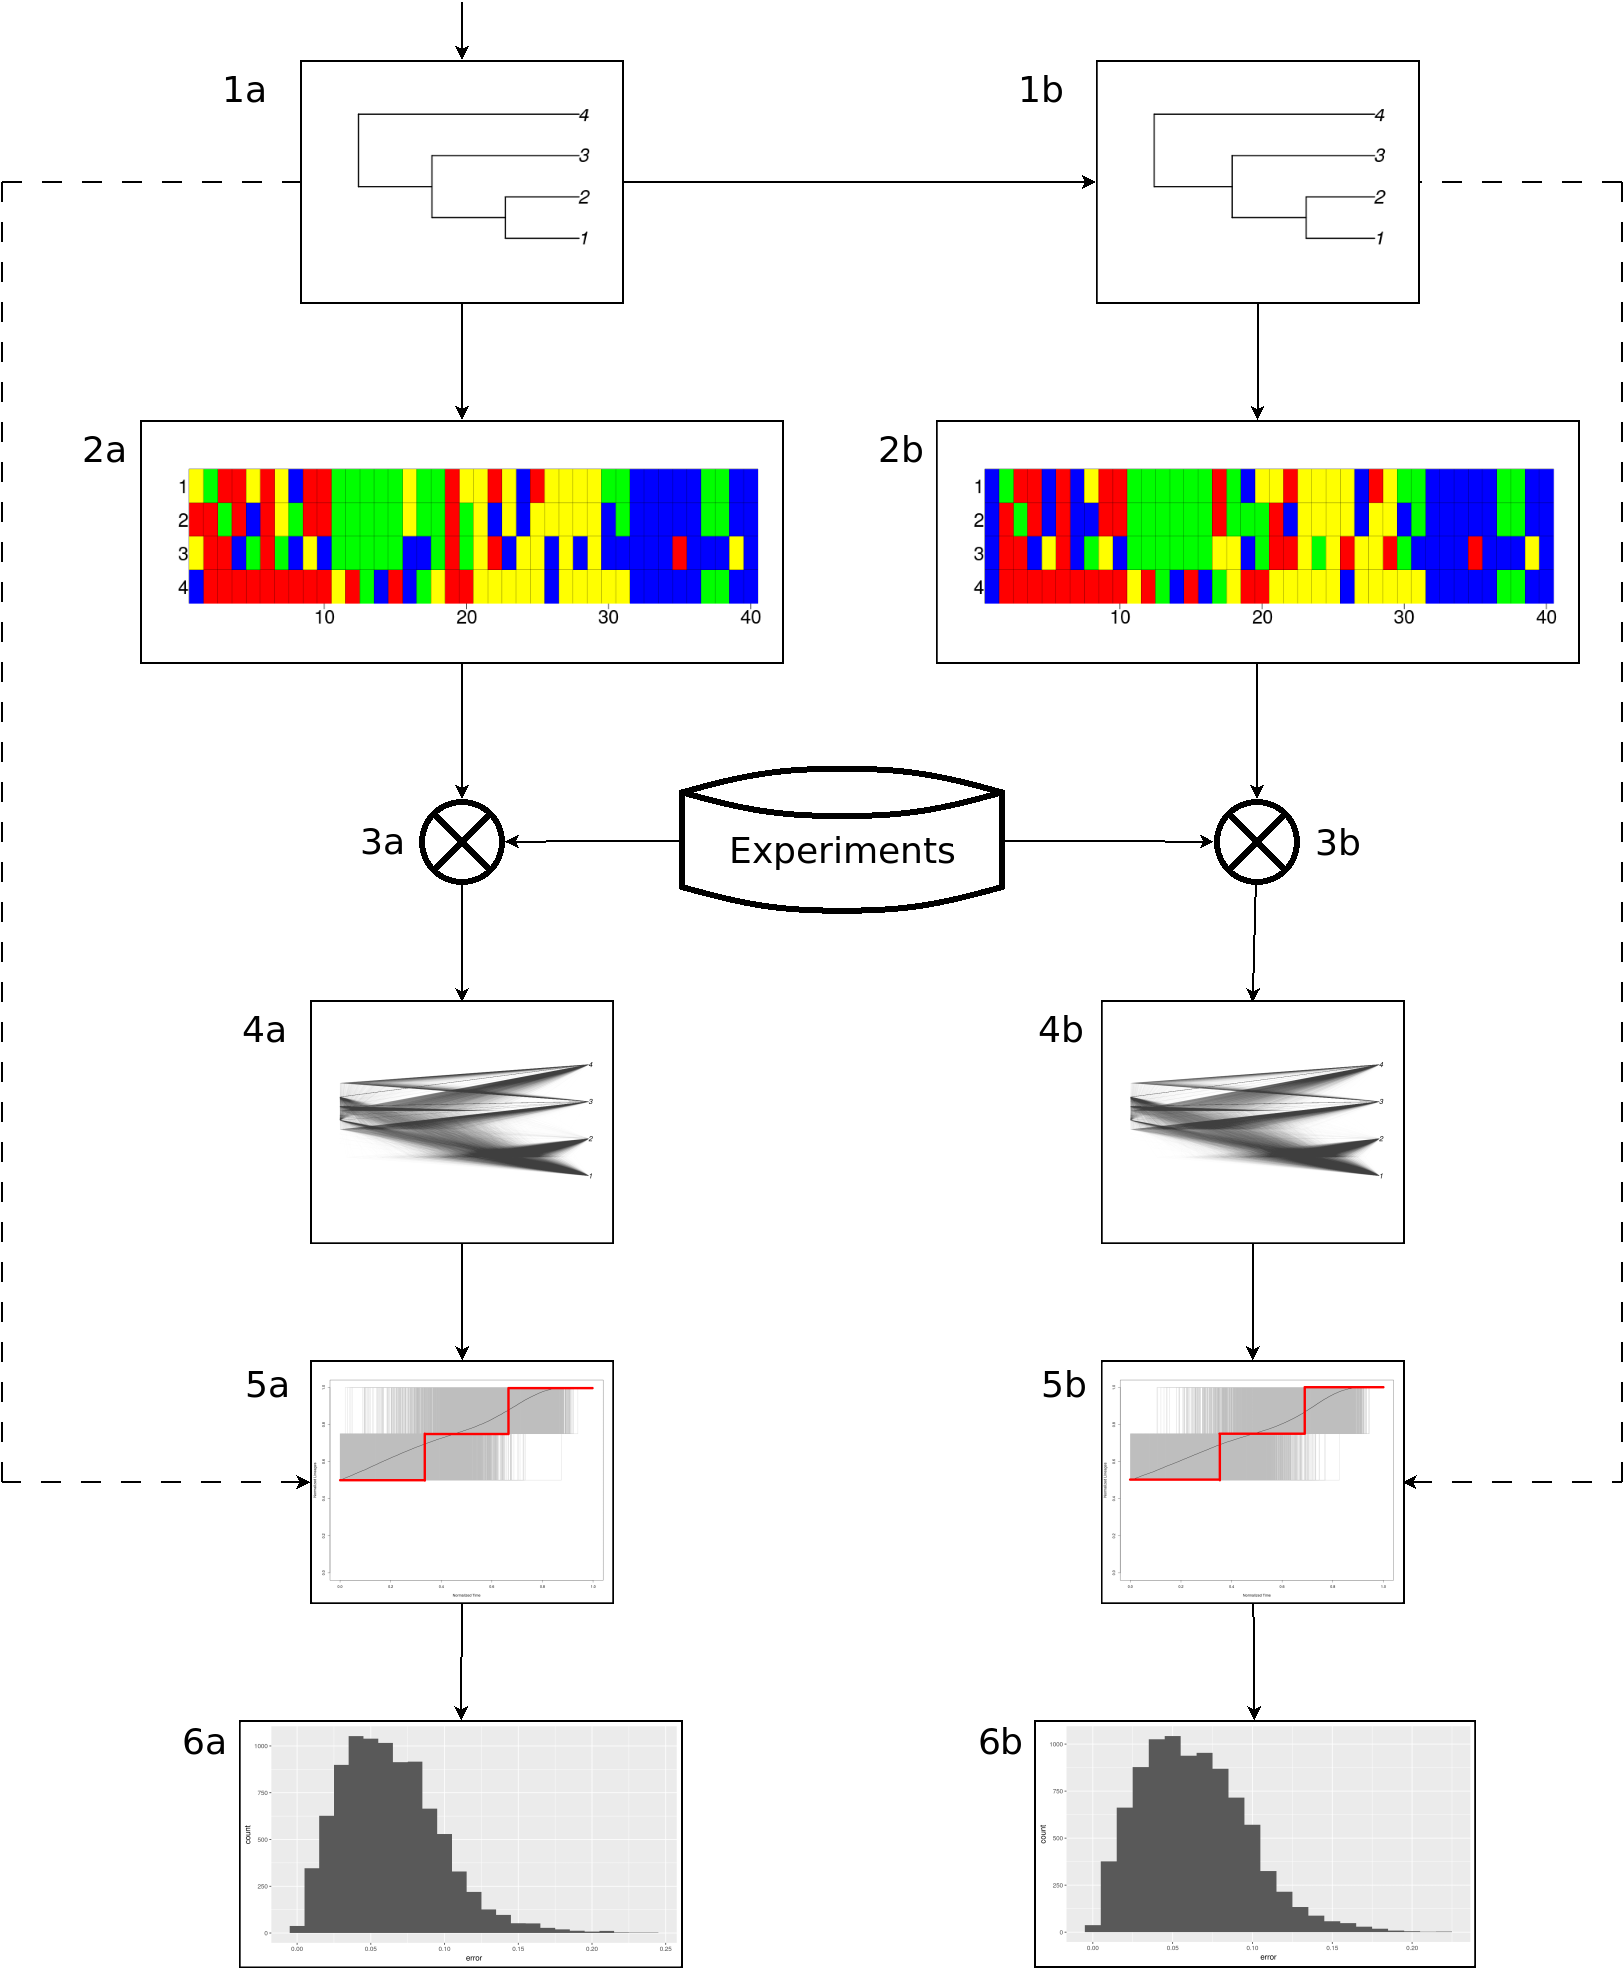
\includegraphics[width=\textwidth]{workflow.png}
  \caption{
    \texttt{pirouette} pipeline. 
    The pipeline starts from a phylogeny (1a) simulated by generative prior 
$\mathit{P}$.
    The phylogeny is converted to an alignment (2a) using alignment model 
$\mathit{A}$. 
    The user supplies one or more experiments.
    For each candidate experiment $\mathit{X}$ 
    (a tuple of inference model $\mathit{I}$ and condition $\mathit{C}$),
    if its condition $\mathit{C}$ is 
    satisfied (which can depend on the alignment), 
    it becomes a selected experiment $\mathit{X'}$, 
    to be used in the next step (3a).
    The inference models of the selected experiment use the alignment (2a) 
    to each create a Bayesian posterior of (parameter estimates and) 
    phylogenies (4a). 
    Each of the posteriors' trees is compared to the true phylogeny (1a) 
    using error measure $\mathit{E}$, 
    resulting in an error distribution (5a). 
    Optionally, a twin phylogeny (1b) can be generated from the original 
    phylogeny (1a) using twinning parameters $T$, where $T$ may depend on
    the experiments \richel{improve}.
    From a twin phylogeny, the same intermediate steps are taken,
    resulting in a twin error distribution (5b)
    \giovanni{Ok, that's my take on this: 1) all the capital letters should go 
in a ball (or a rhombus, as you already did for C) which stands in the middle 
of the arrows (as with C now); 2) The box in the middle should contain all the 
inference models $I_{i}$; 3) We need another C at the intersection of the 
arrows that point to T and A; 4) In between of the arrow 2a->4a there should be 
another rhombus (or circle) with an I (or I' or I*, according on how we want to 
call the selected inference model), which is pointed by the rhombus (of circle) 
containing C; 5) The first arrow should start from a rhombus (or circle) with P 
inside.}
  }
  \label{fig:pipeline}
\end{figure}

The pipeline is summarized by the following steps:
\begin{enumerate}
    \item for a given phylogeny an alignment is simulated under a known 
alignment model;
    \item for this alignment, according to the specified inference conditions, 
an inference model is picked (which may be different from the generative 
alignment model);
    \item the alignment is then used as BEAST2 input to infer a posterior 
distribution of phylogenies;
    \item posterior phylogenies are compared with the given original phylogeny 
to estimate the error made, according to the error measure specified by the 
user;
\end{enumerate}
The pipeline is visualized in Fig.~\ref{fig:pipeline}. 
There is also the option to generate a 'twin tree', 
that goes through the same pipeline. 
The utility of this twin tree will be explained below.

The first step simulates a DNA alignment from a given 
phylogeny (Fig.~\ref{fig:pipeline}, 1a $\rightarrow$ 2a).
This operation is performed according to the alignment model 
specified by the user, which consists in a root DNA sequence, 
a DNA mutation rate and a site model.
A strict clock model is used as the only clock model
type, as the currently used alignment simulation algorithm
only supports a mutation rate that is equal across all the branches.
This step is relatively fast, 
but longer DNA alignments will noticeably slow down the inference step.

The second step (Fig.~\ref{fig:pipeline}, 2a $\rightarrow$ 3a)
starts from experiments as set up by the user. 
We define an experiment as the combination of an inference model 
and the conditions to actually use it in the inference step.
The inference model can be selected in two ways, either using the
generative model or selecting one or more candidates out of a list of candidate 
inference models.
An experiment can use the generative model as the inference model, if the 
generative model is known.
An experiment uses a candidate model if either the generative model is unknown,
or there is an interest in seeing how well non-generative models compete with
the generative model.
Typically, a generative model and/or a best candidate model are used in the 
actual inference.
When using an experiment with a generative model,
it must use the same site and clock model used in the alignment simulation,
as well as the tree prior that underlied the creation of the given phylogeny. 
When using experiments with candidate models,
\verb;pirouette; selects the best candidate based
on the evidence (i.e. marginal likelihood) for the model given the alignment.
The evidence of an inference model is estimated using a nested sampling (NS)
approach, as described in \cite{maturana2018model}. The nested sampling is
performed by \verb;mcbette; [\cite{mcbette}], that calls the 'NS' BEAST2 
package. 
Using BEAST2 packages (in a scripted way) can only be done under Linux and Mac,
therefore the selection of candidate models is not available directly on 
Windows. 
However, even on Windows systems there is the option to perform the model 
selection from browser, using \verb;mcbette;, yet the computation for this 
model selection is
restricted to one hour for free users of the host (Travis CI) continuous
integration service.

The third step infers the actual Bayesian posteriors from the simulated 
alignment (Fig.~\ref{fig:pipeline}, 2a $\rightarrow$ 3a $\rightarrow$ 4a),
using the inference models from the experiments selected in the previous step. 
For each selected experiment, one BEAST2 posterior is inferred, using the 
\verb;babette; [\cite{bilderbeek2018babette}] R package.

The fourth step compares the true tree to each posterior tree, resulting in an 
error distribution (Fig.~\ref{fig:pipeline}, 4a $\rightarrow$ 5a).
The nLTT statistic (\cite{janzen2015approximate}) is used by default, but also 
a user-defined error statistic can be used. 
As an example, \verb;pirouette; supplies one custom error statistic,
that uses an absolute difference in the gamma statistic 
[\cite{pybus2000testing}].
Additionally, the user can specify the proportion of posterior phylogenies to 
discard (i.e. the burn-in), throwing away the first $10\%$
of all phylogenies by default. This burn-in is used to discard
the part of the MCMC chain that has not yet converged to a
representative part of the state space.

\subsection{Twin tree}\label{subsec:twinning}

An optional step is to generate a 'twin tree' $\tau_{I}$
(Fig.~\ref{fig:pipeline}, 1a $\rightarrow$ 1b),
that will be analyzed in the same way as the true tree, following a parallel 
pipeline. We want to produce such tree 'converting' the original tree 
$\tau_{\mathit{P}}$, created according to the generative prior $\mathit{P}$, to 
be in accordance with the chosen inference model $\mathit{I}$:
\begin{align}
    \tau_{\mathit{P}} = (\Vec{t}_{\mathit{P}}, \psi_{\mathit{P}}) 
\xrightarrow[]{\mathit{T}} \tau_{\mathit{I}} = (\Vec{t}_{\mathit{I}}, 
\psi_{\mathit{I}}),
\end{align}
where $\Vec{t}$ are the tree branching times and $\psi$ is tree topology, which 
provides information on where new lineages branch out at each branching time.

To execute the twinning process we exploit the likelihood function 
$L_{\mathit{I}}$ associated with the chosen inference model $\mathit{I}$. We 
find the parameters $\theta^{*}_{\mathit{I}}$ (e.g. speciation and extinction 
rates, in case of a birth-death model) that maximize $L_{\mathit{I}}$ applied 
to the true tree, conditioned on its number of tips $n_{\mathit{P}}$,
\begin{align}
    max[L_{\mathit{I}}(\theta_{\mathit{I}}|\tau_{\mathit{P}}, n_{\mathit{P}})] 
\rightarrow \theta^{*}_{\mathit{I}}.
\end{align}
We use $\theta^{*}_{\mathit{I}}$ to simulate an equal amount $n_{\mathit{I}} = 
n_{\mathit{P}}$ of branching times $\Vec{t}_{\mathit{I}}$ for the twin tree 
$\tau_{\mathit{I}}$, under the process $\mathit{I}$. We then impose that 
$\tau_{\mathit{P}}$ and $\tau_{\mathit{I}}$ must respect the same topology
\begin{align}
    \psi_{\mathit{I}} = \psi_{\mathit{P}}.
\end{align}
Using a twin tree serves as a control: both $\tau_{\mathit{P}}$ and 
$\tau_{\mathit{I}}$ will produce an error distribution. We assume that these 
errors are a natural product of the input tree and the intermediate steps of 
the pipeline. All the factors that can cause such errors are: the branching 
times $\vec{t}$ of the tree (as a consequence of the tree prior), its topology 
$\psi$, the stochasticity induced by simulating the alignment (step 1a 
$\rightarrow$ 2a in Fig.~\ref{fig:pipeline}) and the stochasticity induced by 
the Bayesian inference (step 2a $\rightarrow$ 4a in Fig.~\ref{fig:pipeline}). 
By imposing the same topology and replicating the pipelines a sufficient number 
of times we can sort out all the possible causes that are not a direct 
consequence of the choice of the tree prior.

Potential differences in shape of error distributions will therefore be 
consequences of different tree priors for the two parallel pipelines: the use 
of prior $\mathit{P}$ for the original pipeline and of prior $\mathit{I}$ for 
the twin pipeline. In the second case, though, such error distribution is not 
influenced by the mismatch between how the tree is generated and how it is 
analyzed by BEAST2.
%%%%%%%%%%%%%%%%%%%%%%%%%%%%%%%%%%%%%%%%%%%%%%%%%%%%%%%%%%%%%%%%%%%%%%%%%%%%%%%%
\section{Installation}
%%%%%%%%%%%%%%%%%%%%%%%%%%%%%%%%%%%%%%%%%%%%%%%%%%%%%%%%%%%%%%%%%%%%%%%%%%%%%%%%

\verb;pirouette; can be installed easily from CRAN:
\begin{lstlisting}[language=R, floatplacement=ht, frame=single]
install.packages("pirouette")
\end{lstlisting}

For the most up-to-date version, 
one can download and install the package from \verb;pirouette;'s GitHub 
repository:

\begin{lstlisting}[language=R, floatplacement=ht, frame=single]
usethis::install_github("richelbilderbeek/pirouette")
\end{lstlisting}

To start using \verb;pirouette;, load its functions in the global namespace 
first:

\begin{lstlisting}[language=R, floatplacement=ht, frame=single]
library(pirouette)
\end{lstlisting}
Because \verb;pirouette; calls BEAST2, BEAST2 must be installed. 
This can be done from within R, using:

\begin{lstlisting}[language=R, floatplacement=ht, frame=single]
install_beast2()
\end{lstlisting}
For the option to select a best candidate model,
\verb;pirouette; needs the "NS" BEAST2 package [\cite{maturana2018model}].
It can be installed from within R, using:

\begin{lstlisting}[language=R, floatplacement=ht, frame=single]
install_beast2_pkg("NS")
\end{lstlisting}

An overview of \verb;pirouette;'s main functions is shown in 
table~\ref{tab:functions}. 
These functions are demonstrated when in the example code below.
All \verb;pirouette;'s functions are documented,
have a useful example, and have sensible defaults.

%%%%%%%%%%%%%%%%%%%%%%%%%%%%%%%%%%%%%%%%%%%%%%%%%%%%%%%%%%%%%%%%%%%%%%%%%%%%%%%%
\begin{table}[h]
\centering
\begin{tabular}{ | l | l | }
\hline
\textbf{Name} & \textbf{Description} \\
\hline
\verb;pir_run; & Run \verb;pirouette; \\
\verb;create_pir_params; & Create the \verb;pirouette; parameters \\
\hline
\verb;create_alignment_params; & Create the alignment parameters \\
\verb;create_twinning_params; & Create the twinning parameters \\
\verb;create_experiment; & Create one experiment \\
\verb;create_error_measure_params; & Create the error measurement parameters \\
\hline
\end{tabular}
\caption{pirouette's main functions.}
\label{tab:functions}
\end{table}
%%%%%%%%%%%%%%%%%%%%%%%%%%%%%%%%%%%%%%%%%%%%%%%%%%%%%%%%%%%%%%%%%%%%%%%%%%%%%%%%

%%%%%%%%%%%%%%%%%%%%%%%%%%%%%%%%%%%%%%%%%%%%%%%%%%%%%%%%%%%%%%%%%%%%%%%%%%%%%%%%
\section{Usage: Example Research Question 1}
%%%%%%%%%%%%%%%%%%%%%%%%%%%%%%%%%%%%%%%%%%%%%%%%%%%%%%%%%%%%%%%%%%%%%%%%%%%%%%%%

\subsection{Question}

\verb;pirouette; quantifies the influence of a new tree prior on BEAST2's 
inference,
by measuring the difference between a given tree and 
phylogenies in a posterior. Due to stochasticity, all posterior trees
will differ from the given phylogeny, even when the generative tree
prior $\mathit{P}$ and alignment model $\mathit{A}$ are the same as 
those in the inference model $\mathit{I}$.
Measuring this difference allows us to know the baseline error
of the \verb;pirouette; pipeline. We therefore define as 'standard tree priors' 
all the tree priors that are available to be used within an inference model 
(see Table~\ref{tab:options}).

Now we can formulate the first example research question that \verb;pirouette; 
can answer:

"What is the inference error made on phylogenies
created by a standard diversification model?"

\subsection{Answer}

In this example we use a standard generative tree prior $\mathit{P_{0}}$, 
namely the Yule (pure-birth) tree prior. 
We choose to use a small tree with six taxa to keep
the calculations short and the figure more readable.
We pick a crown age of ten time units. This value is 
completely arbitrary, but does tie in with the mutation rate 
used in simulating an alignment in the next step.

\begin{lstlisting}[
    language=R, floatplacement=ht, frame=single, 
    label = {lst:create_yule_tree}, 
    caption = {
      Create a Yule tree. 
      The resulting tree is shown in figure~\ref{fig:yule_tree}.
    }
  ]
phylogeny <- create_yule_tree(n_taxa = 6, crown_age = 10)
\end{lstlisting}

\begin{figure}[ht]
  \includegraphics[width=\textwidth]{example_1/true_tree.png}
  \caption{The Yule tree, as created by listing~\ref{lst:create_yule_tree}.}
  \label{fig:yule_tree}
  \giovanni{Remove the text in top-left corner.}
  \richel{Agreed, iff the text matches the code}
  \giovanni{I'd use a sexier topology, purely for esthetical reasons.}
  \richel{Agreed, will pick a sexy RNG seed after create\_yule\_tree is there}
\end{figure}

The first step in \verb;pirouette; is to simulate a DNA alignment from the 
given phylogeny. 
To do so, we must specify an alignment model $\mathit{A}$ which consists of: a 
DNA root sequence $\mathit{r_{s}}$, the DNA mutation rate $\mathit{m_{r}}$, a
site model $\mathit{s_{m}}$ (in this context: a nucleotide substitution model) 
and a clock model $\mathit{c_{m}}$. 
In this example, the DNA root sequence consists in four blocks of 250 
nucleotides each, 
where the per-nucleotide mutation rate is 0.1 mutations per unit time.
We use a Jukes-Cantor (JC, \cite{jukes1969evolution}) site model
and a strict clock model as these are the simplest.
A Jukes-Cantor site model
assumes that mutation rates between nucleotides are equal and constant. 
A strict clock model assumes that the mutation rates 
of all species are equal and constant.

\begin{lstlisting}[
    language=R,
    floatplacement=ht, frame=single,
    label = {lst:create_alignment}, 
    caption = {Create an alignment.}
  ]
alignment_params <- create_alignment_params(
  root_sequence = create_blocked_dna(length = 1000),
  mutation_rate = 0.1,
  site_model = create_jc69_site_model(),
  clock_model = create_strict_clock_model()
)
\end{lstlisting}

As the site and clock models used here are also the defaults, 
these function arguments can be safely omitted: we just show these
explicitly for clarity.

In the second step we state our experiment.
We define an experiment $\mathit{X}$ as a combination of an inference model 
$\mathit{I}$
and conditions $\mathit{C}$.
In this example we pick $\mathit{I}$ to be the same inference model as the 
generative one,
which is the chosen Yule tree prior $\mathit{P_{0}}$, as well as site and clock 
models defined in $\mathit{A}$, respectively JC and strict.
We specify in $\mathit{C}$ that the experiment will always be run.

\begin{table}
  \begin{tabular}{ | c | c | c | l | }
    \hline
    \textbf{model type} & \textbf{run if} & \textbf{measure evidence} & 
\textbf{inference model} \\ 
    \hline
    generative & always & no & JC, strict, Yule \\
    \hline
  \end{tabular}
  \caption{
    Inference conditions and inference model for ERQ 1.
    JC: Jukes-Cantor site model.
    strict: strict clock model.
    Yule: Yule (pure-birth) tree prior.
  }
  \label{tab:RQ1}
\end{table}

Listing~\ref{lst:create_generative_experiment_explicit} shows how to
set up this experiment:

\begin{lstlisting}[
  language=R, 
  floatplacement=ht, frame=single,
  label = {lst:create_generative_experiment_explicit},
  caption = {
    Create the experiments to answer research question 1, 
    using explicit arguments
  }
]
experiment <- create_experiment(
  inference_conditions = create_inference_conditions(
    model_type = "generative", 
    run_if = "always"
  ), 
  inference_model = create_inference_model(
   site_model = create_jc69_site_model(), 
   clock_model = create_strict_clock_model(), 
   tree_prior = create_yule_tree_prior()
  )
)
\end{lstlisting}

Experiments must be bundled in a list to work, even if only one is provided, as 
in this case:

\begin{lstlisting}[
  language=R, 
  floatplacement=ht, frame=single,
  label = {lst:create_generative_experiment},
  caption = {
    Create the experiments to answer research question 1.
  }
]
experiments <- list(experiment)
\end{lstlisting}

The objects we just created need to be bundled
in a \verb;pirouette; parameters structure,
together with error measurement parameters $\mathit{E}$ and
twinning parameters $\mathit{T}$. 

We use the default error measurement
parameters, which uses a burn-in of 10\% and the nLTT statistic to
measure the difference between phylogenies. For clarity,
we create this setup explicitly here:

\begin{lstlisting}[
  language=R, floatplacement=ht, frame=single,
  label = {lst:create_error_measure_params},
  caption = Calling \texttt{create\_error\_measure\_params}
]
error_measure_params <- create_error_measure_params(
  burn_in_fraction = 0.1, 
  error_function = get_nltt_error_function()
)
\end{lstlisting}

We will not use twinning
here yet.  
All these arguments are bundled
and checked by \verb;create_pir_params;:

\begin{lstlisting}[
  language=R, floatplacement=ht, frame=single,
  label = {lst:create_pir_params},
  caption = Calling \texttt{create\_pir\_params}
]
pir_params <- create_pir_params(
  alignment_params = alignment_params,
  experiments = experiments,
  error_measure_params = error_measure_params,
  twinning_params = NA
)
\end{lstlisting}

Now we can use our Yule tree and \verb;pir_params; to measure 
the inference error made on phylogenies
created by a standard diversification model:

\begin{lstlisting}[
  language=R, floatplacement=ht, frame=single,
  label = {lst:pir_run},
  caption = Calling \texttt{pir\_run}
]
errors <- pir_run(
  phylogeny = phylogeny,
  pir_params = pir_params
)
\end{lstlisting}

The error distribution returned by \verb;pir_run; is stored as a data frame. 
\richel{
  I suggest \texttt{pir\_run} to return a list of run experiments,
  as described in Issue 225, 
  \url{https://github.com/richelbilderbeek/pirouette/issues/225}
}
It can be directly plotted using \verb;pir_plot;:

\begin{lstlisting}[
  language=R, floatplacement=ht, frame=single,
  label = {lst:pir_plot},
  caption = Calling \texttt{pir\_plot}
]
pir_plot(errors)
\end{lstlisting}

\begin{figure}[ht]
  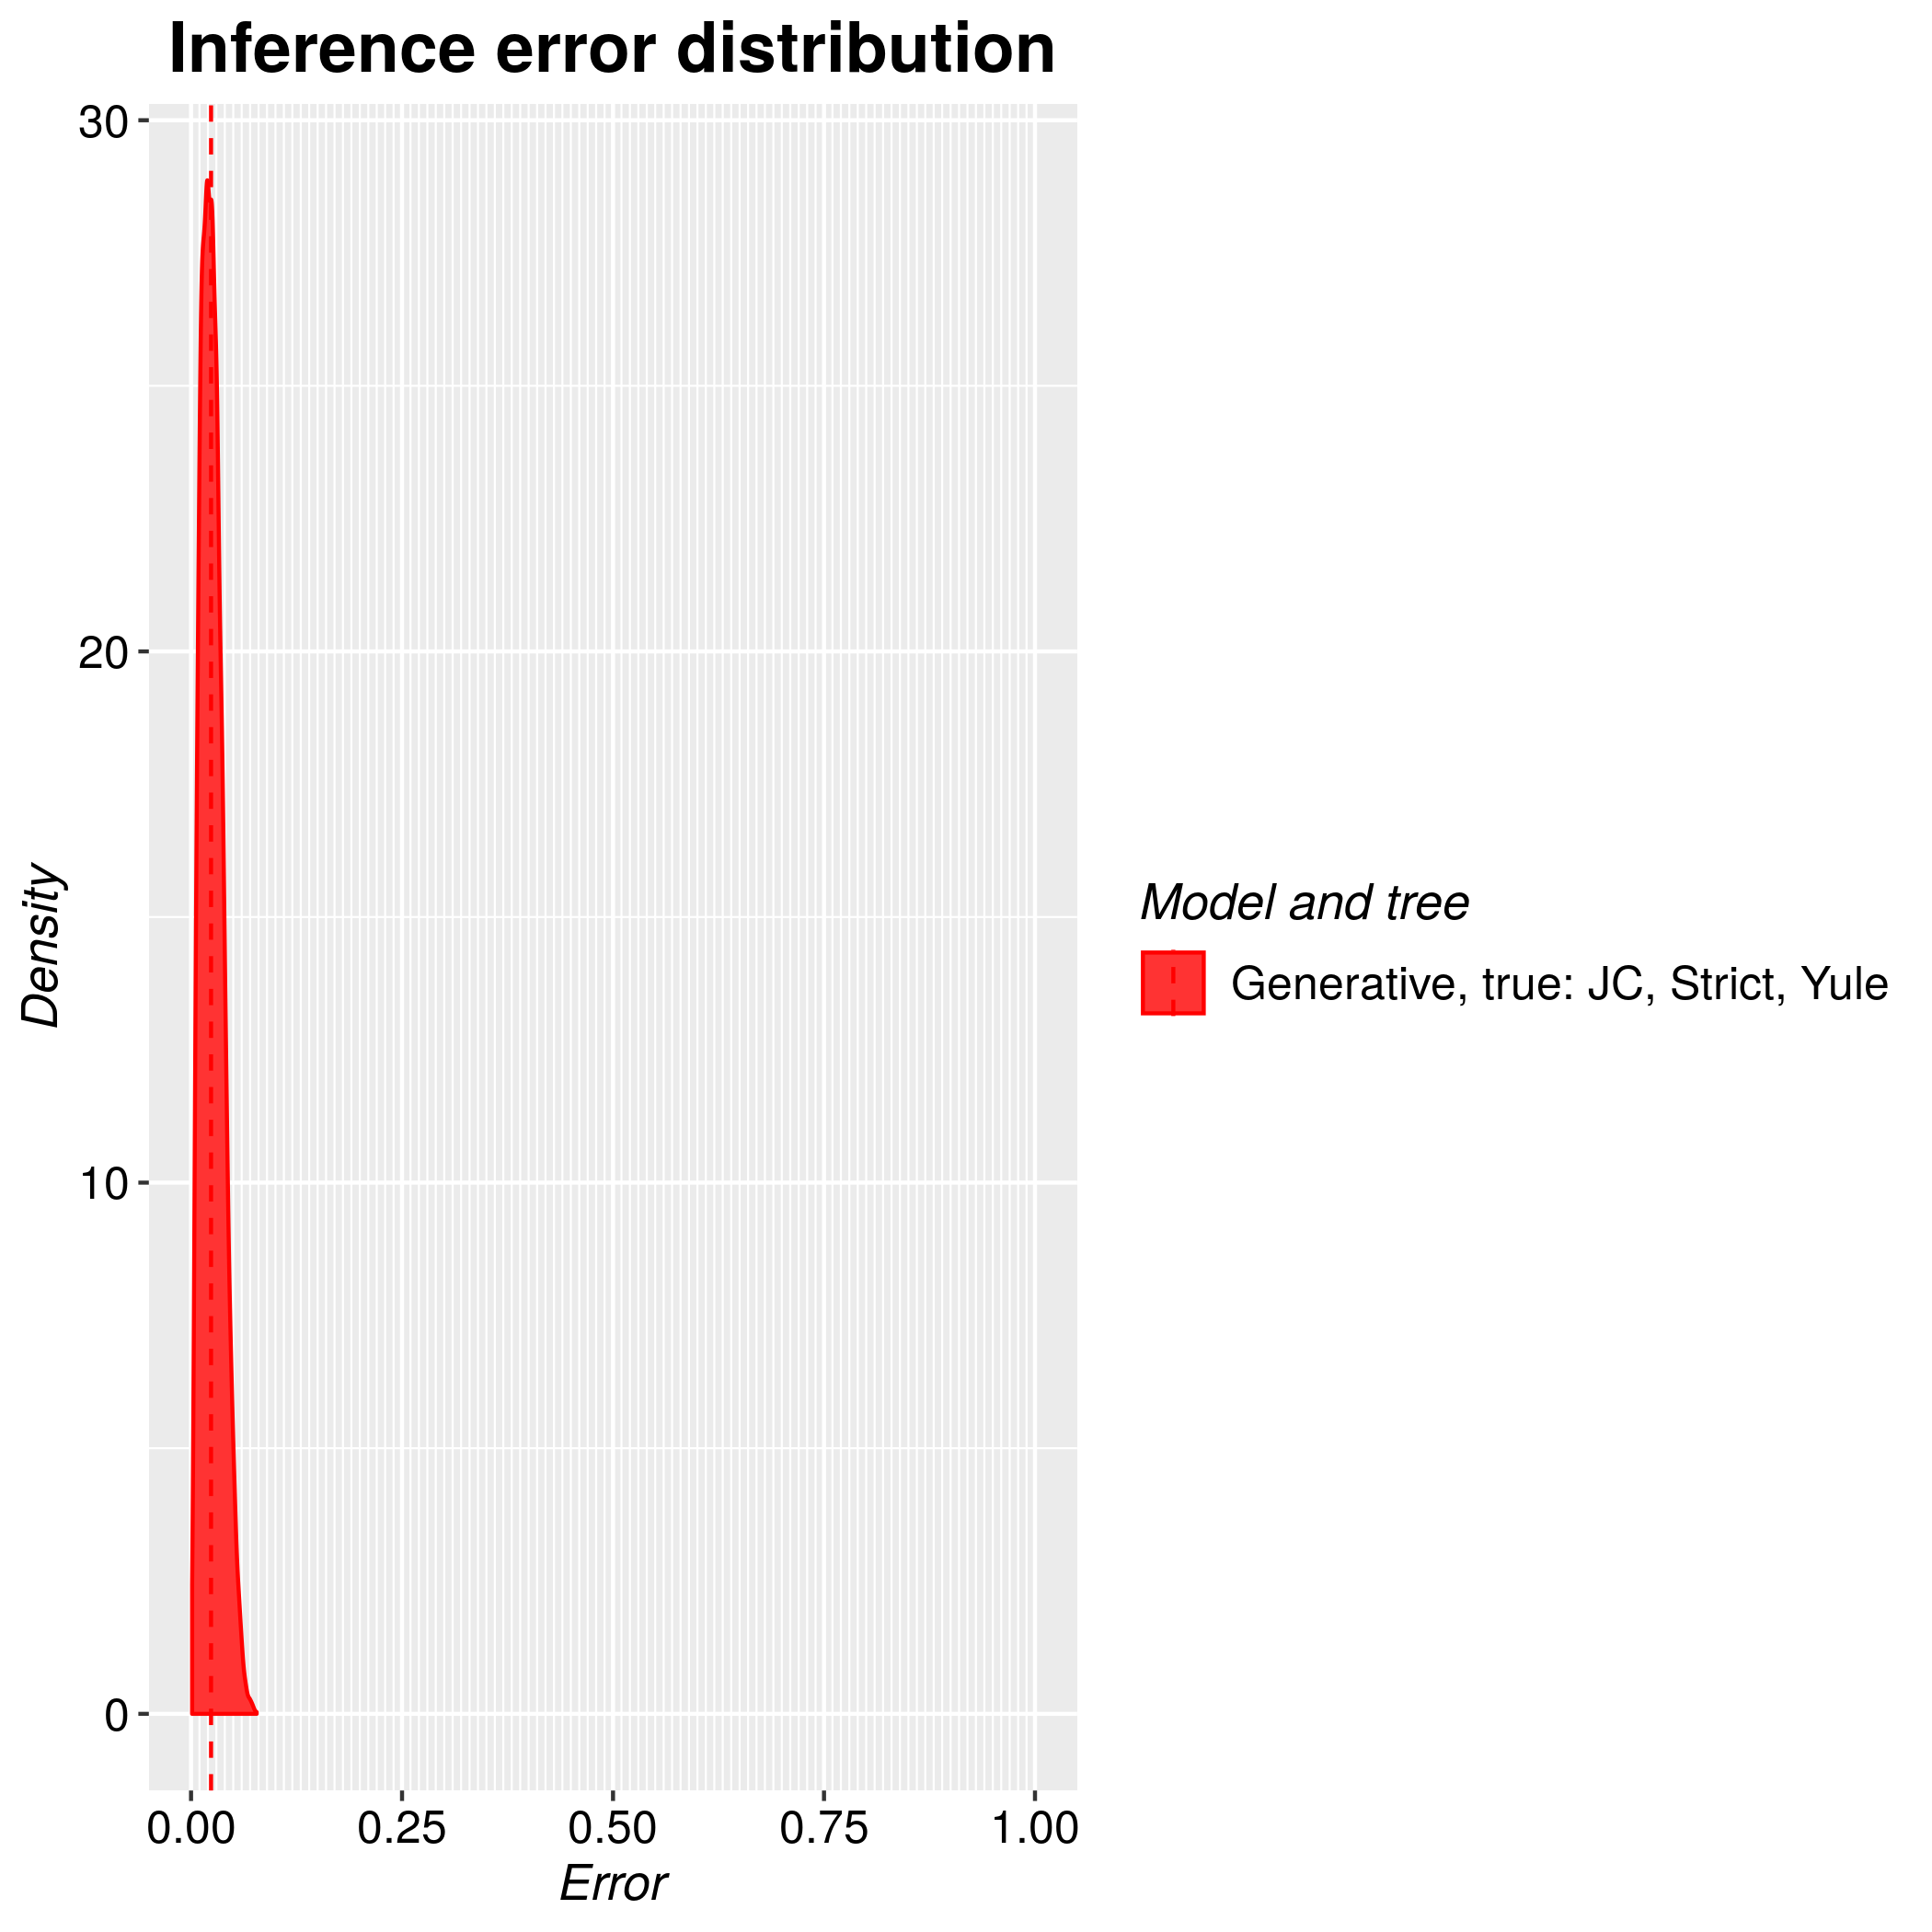
\includegraphics[width=\textwidth]{example_1/errors.png}
  \caption{
    Example 1: the error BEAST2 makes from a phylogeny 
    when the generative and inference model are the same.
  }
  \label{fig:example_1}
\end{figure}

The error distribution obtained is shown as a violin plot
in figure~\ref{fig:example_1}
\richel{
  I suggest to use a histogram (or density plot) instead:
  I like how the error distribution in figure 1 looks.
}
. 

This error distribution has little relevance on its own, 
as we constructed the experiment in such a way $\mathit{I}$ 
matches with the generative model given by $\mathit{A}$ and $\mathit{P_{0}}$.
However it will become clear when compared to the errors obtained from a 
phylogeny 
derived from a non-standard diversification process $\mathit{P}$.

By doing so, this error distribution will serve as a control,
as it can be seen as the baseline error caused by stochasticity.
If the two error distributions obtained from $\mathit{P_{0}}$ and $\mathit{P}$ 
will appear similar, the error induced by the choice of a non-standard 
speciation process will be of little influence.
Given the necessity of such comparison,
we made it an inherent part of \verb;pirouette;. 
We call it 'twinning' and we use it in ERQ 3.

%%%%%%%%%%%%%%%%%%%%%%%%%%%%%%%%%%%%%%%%%%%%%%%%%%%%%%%%%%%%%%%%%%%%%%%%%%%%%%%%
\section{Usage: Example Research Question 2}
%%%%%%%%%%%%%%%%%%%%%%%%%%%%%%%%%%%%%%%%%%%%%%%%%%%%%%%%%%%%%%%%%%%%%%%%%%%%%%%%

\subsection{Question}

In the previous example we selected the inference model $\mathit{I}$ to match 
with a known generative tree prior $\mathit{P_{0}}$.
However, a novel tree prior $\mathit{P}$, by definition, is non-standard, thus 
cannot be part of a standard inference model (i.e. an inference model using a 
standard tree prior).
In this case the user has to specify the the tree prior $\mathit{t_{p}}$ to be 
used in the inference from a list of standard tree priors. In general, having 
no information on $\mathit{P}$, this choice is arbitrary.
\verb;pirouette; provides two ways to deal with this problem. The choice can be 
made specifying the inference conditions $\mathit{C}$ to be used.

If the user has sufficient reasons to believe that one standard tree prior 
could be more suitable than others for the inference, they can set it as part 
of the inference model and to adopt site and clock models used to simulate the 
alignment. This option can be specified selecting "model\_type" to be 
"generative" as part of the inference conditions (as seen in ERQ 1, 
table~\ref{tab:RQ1}).

If, instead, there is no preference for a specific tree prior, the user can let 
\verb;pirouette; select the best inference model from a list of candidate 
models. The model selection is performed automatically based on the criterion 
of the highest evidence (also known as marginal likelihood). This option can be specified 
providing any number of experiments, selecting "model\_type" to be "candidate" 
for each of them, and "run\_if" to be "best\_candidate" (table~\ref{tab:RQ2} 
will summarize this for ERQ 2).

We show the procedure using \verb;pirouette; to answer the second research 
question:

"What is the inference error made on a novel phylogeny when
picking the best inference model?"

\subsection{Answer}

Here we start with a tree generated from an unknown 
diversification model, that has six taxa and a crown age of ten:

\begin{lstlisting}[
  language=R, 
  floatplacement=ht, 
  frame=single, 
  label = {lst:unknown_phylogeny},
  caption = A phylogeny generated by an unknown diversification model.
]
phylogeny  <- ape::read.tree(
  text = "(((A:8, B:8):1, C:9):1, ((D:8, E:8):1, F:9):1);"
)
\end{lstlisting}
\begin{figure}[ht]
  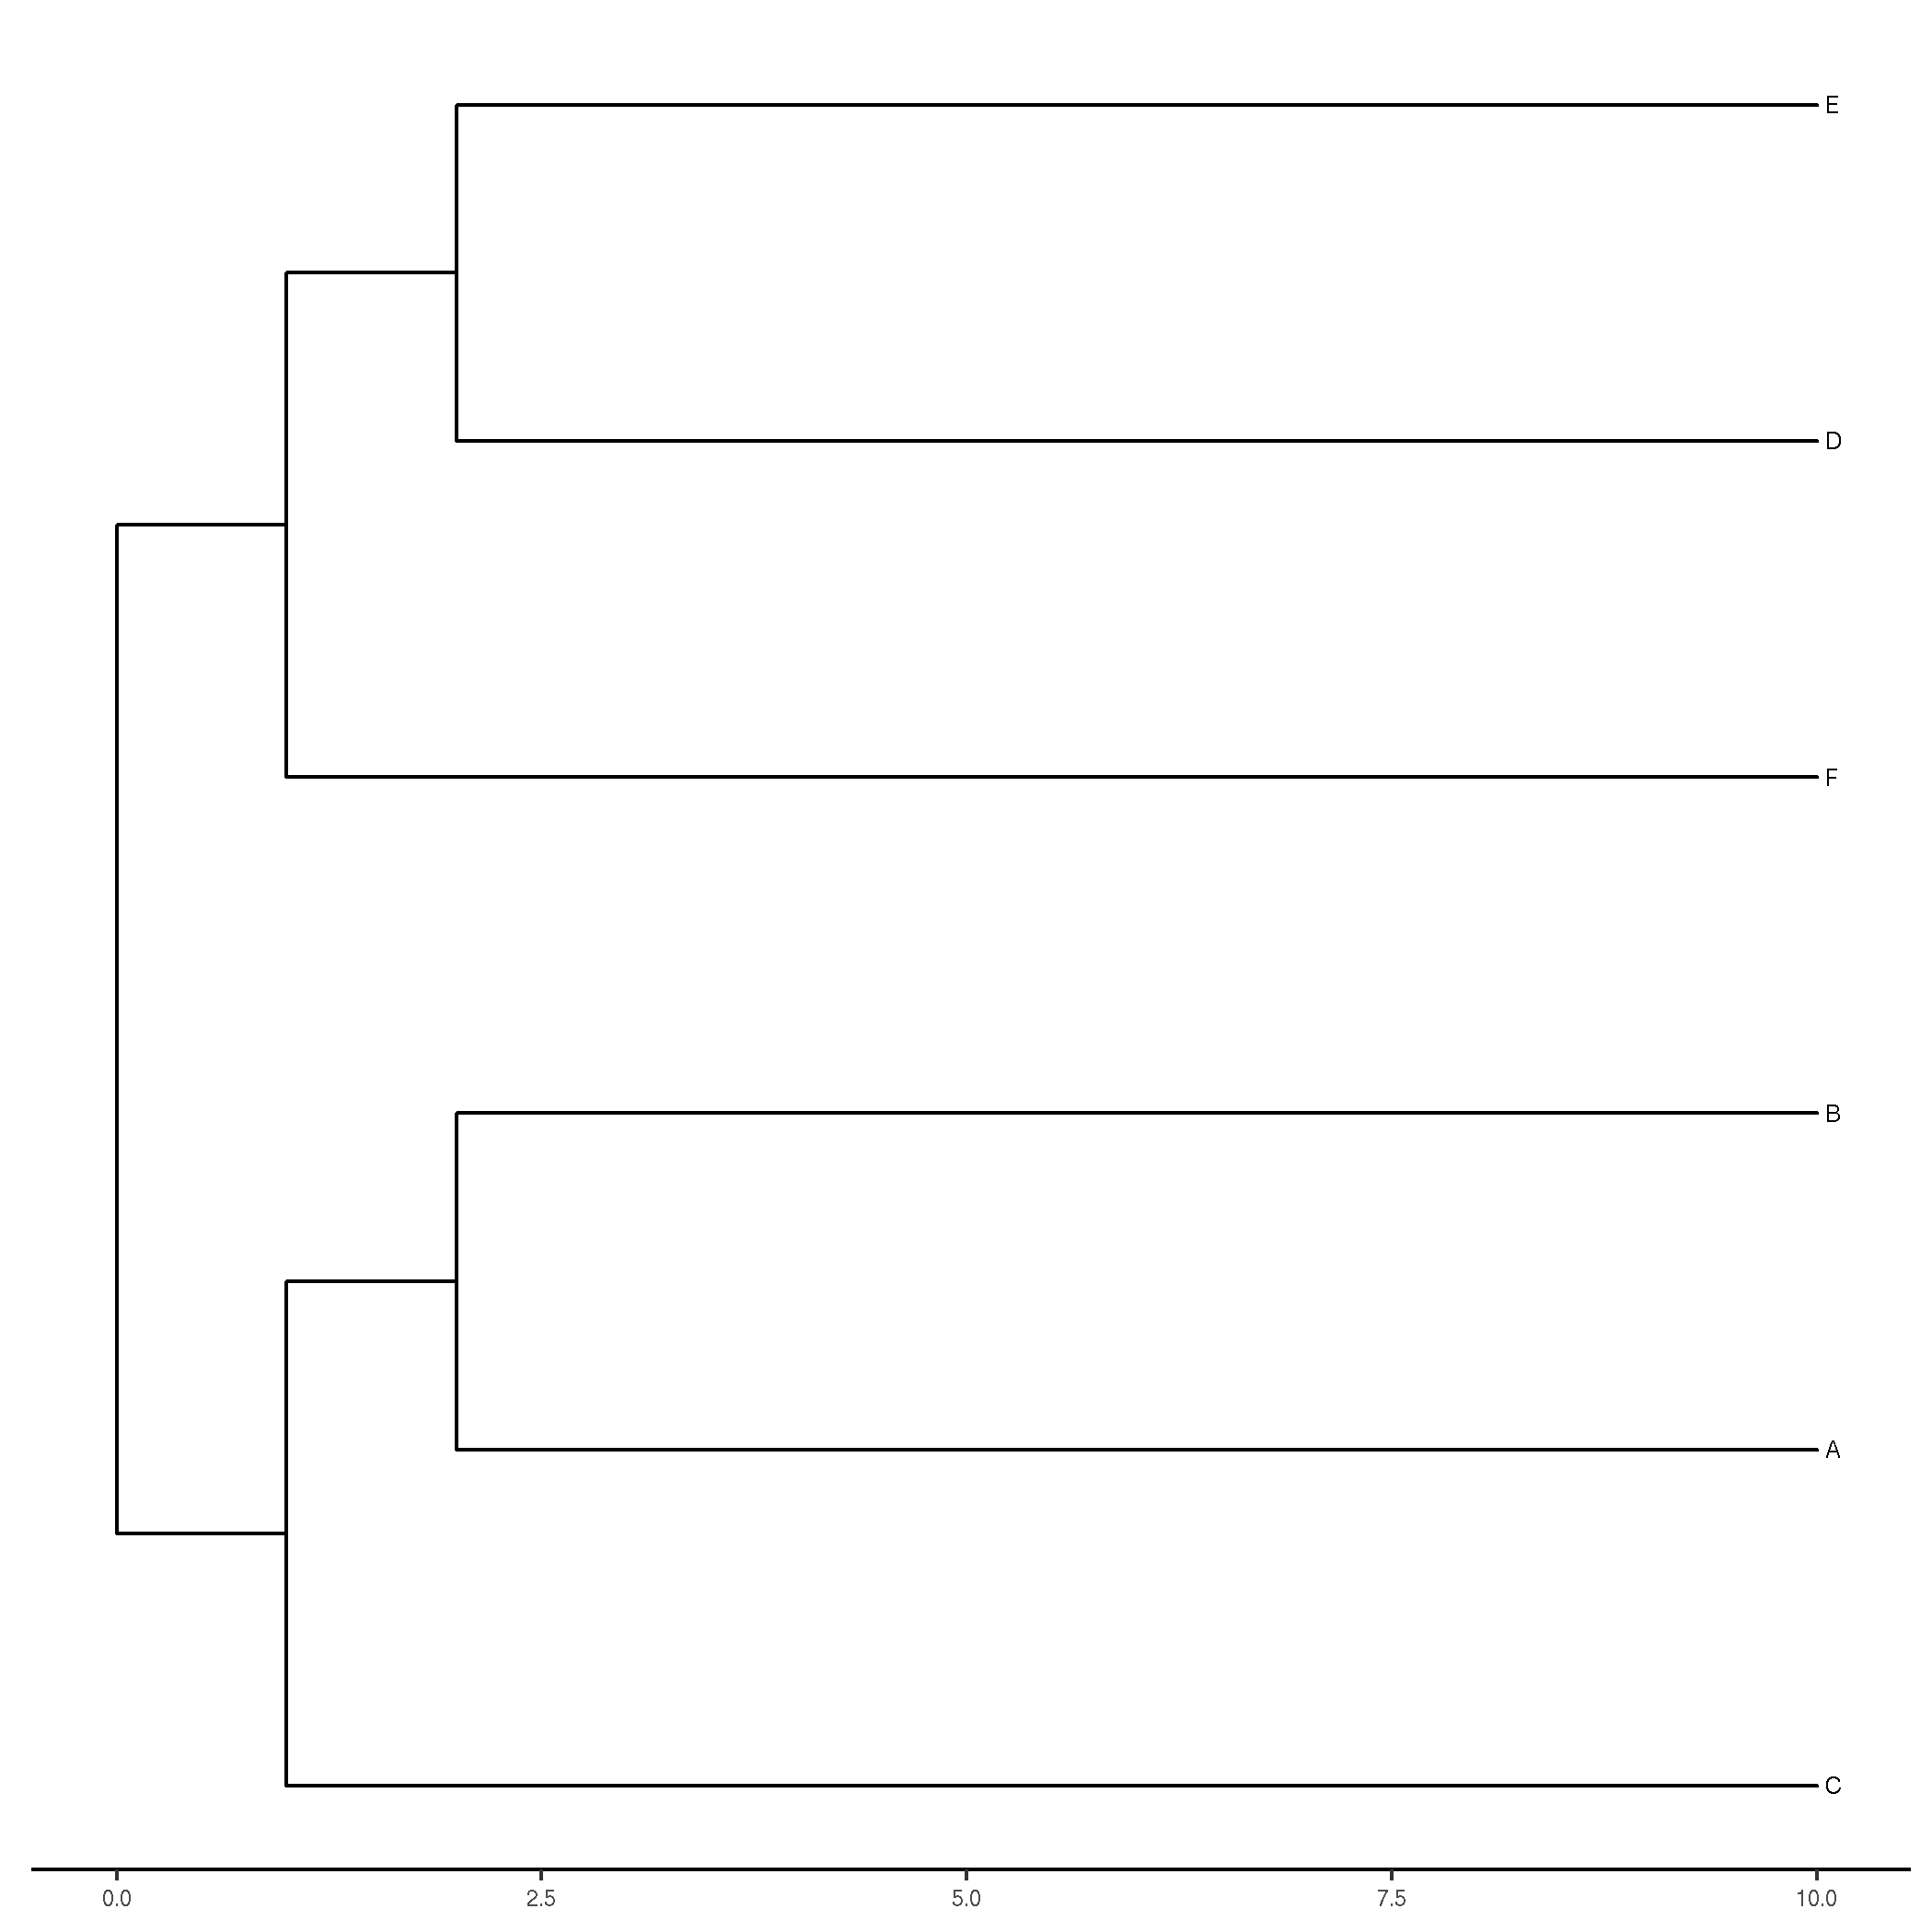
\includegraphics[width=\textwidth]{example_2/tree_unknown.png}
  \caption{The tree derived from an unknown diversification process, 
    as created by listing~\ref{lst:unknown_phylogeny}.
  }
\end{figure}

The first step in \verb;pirouette; is to simulate a DNA alignment from the 
given phylogeny. 
We will re-use the alignment parameters of the previous example 
as shown in listing~\ref{lst:create_alignment}.

\begin{table}
  \begin{tabular}{ | c | c | c | l | }
    \hline
    \textbf{model type} & \textbf{run if} & \textbf{measure evidence} & 
\textbf{inference model} \\ 
    \hline
    candidate & best candidate & yes & JC, strict, Yule \\
    candidate & best candidate & yes & JC, strict, BD   \\
    ...       & ...            & ... & ...              \\
    candidate & best candidate & yes & GTR, RLN, CCP    \\
    candidate & best candidate & yes & GTR, RLN, CEP    \\
    \hline
  \end{tabular}
  \caption{
    Inference conditions and inference model for ERQ 2.
    JC: Jukes-Cantor site model.
    strict: strict clock model.
    Yule: Yule (pure-birth) tree prior.
    BD: birth-death tree prior.
    GTR: GTR site model.
    RLN: relaxed log-normal clock model.
    CCP: coalescent constant-population tree prior.
    CEP: coalescent exponential-population tree prior.
  }
  \label{tab:RQ2}
\end{table}

In the second step we set up our experiments. Unlike ERQ 1, here we provide a 
set of experiments $\{\mathit{X_{i}}\}_{i=1}^{40}$. All the experiments have 
the same inference conditions $\mathit{C_{i}} = \mathit{C}$ but different 
candidate inference models $\mathit{I_{i}}$. Yet, only one of them will be used 
to run the actual inference. According to the specified $\mathit{C}$, 
\verb;pirouette; will measure the evidence for each of them and select  only 
the one with the highest evidence as the best candidate.

As model selection is commonly performed on the full list of available candidate models,
\verb;pirouette; has a dedicated function to provide it:
\verb;create_all_experiments; will create the entire set of 40 experiments,
containing the inference models of all combinations of 4 site 
models, 2 clock models and 5 tree priors.
\giovanni{Do we still want to use CBS, CCP and CEP?}

\begin{lstlisting}[
  language=R, 
  floatplacement=ht, 
  frame=single, 
  label = {lst:create_all_experiments},
  caption = Create all 40 candidate experiments.
]
experiments <- create_all_experiments()
\end{lstlisting}

For all the other steps we use the default setups. 
We can create the complete
\verb;pirouette; parameter set like this (which is the
same as listing~\ref{lst:create_pir_params}, but using the defaults):

\begin{lstlisting}[
  language=R, floatplacement=ht, frame=single,
  label = {lts:create_pir_params_defaults},
  caption = Create a \texttt{pir\_params} with many defaults.
]
pir_params <- create_pir_params(
  alignment_params = alignment_params,
  experiments = experiments
)
\end{lstlisting}

We can now run \verb;pirouette;  with listing~\ref{lst:pir_run}
and plot the results with listing~\ref{lst:pir_plot}.
The resulting figure is shown in figure~\ref{fig:example_2}.

\giovanni{describe winner}
\richel{agreed, after the figures also show it :-) }

\begin{figure}[ht]
  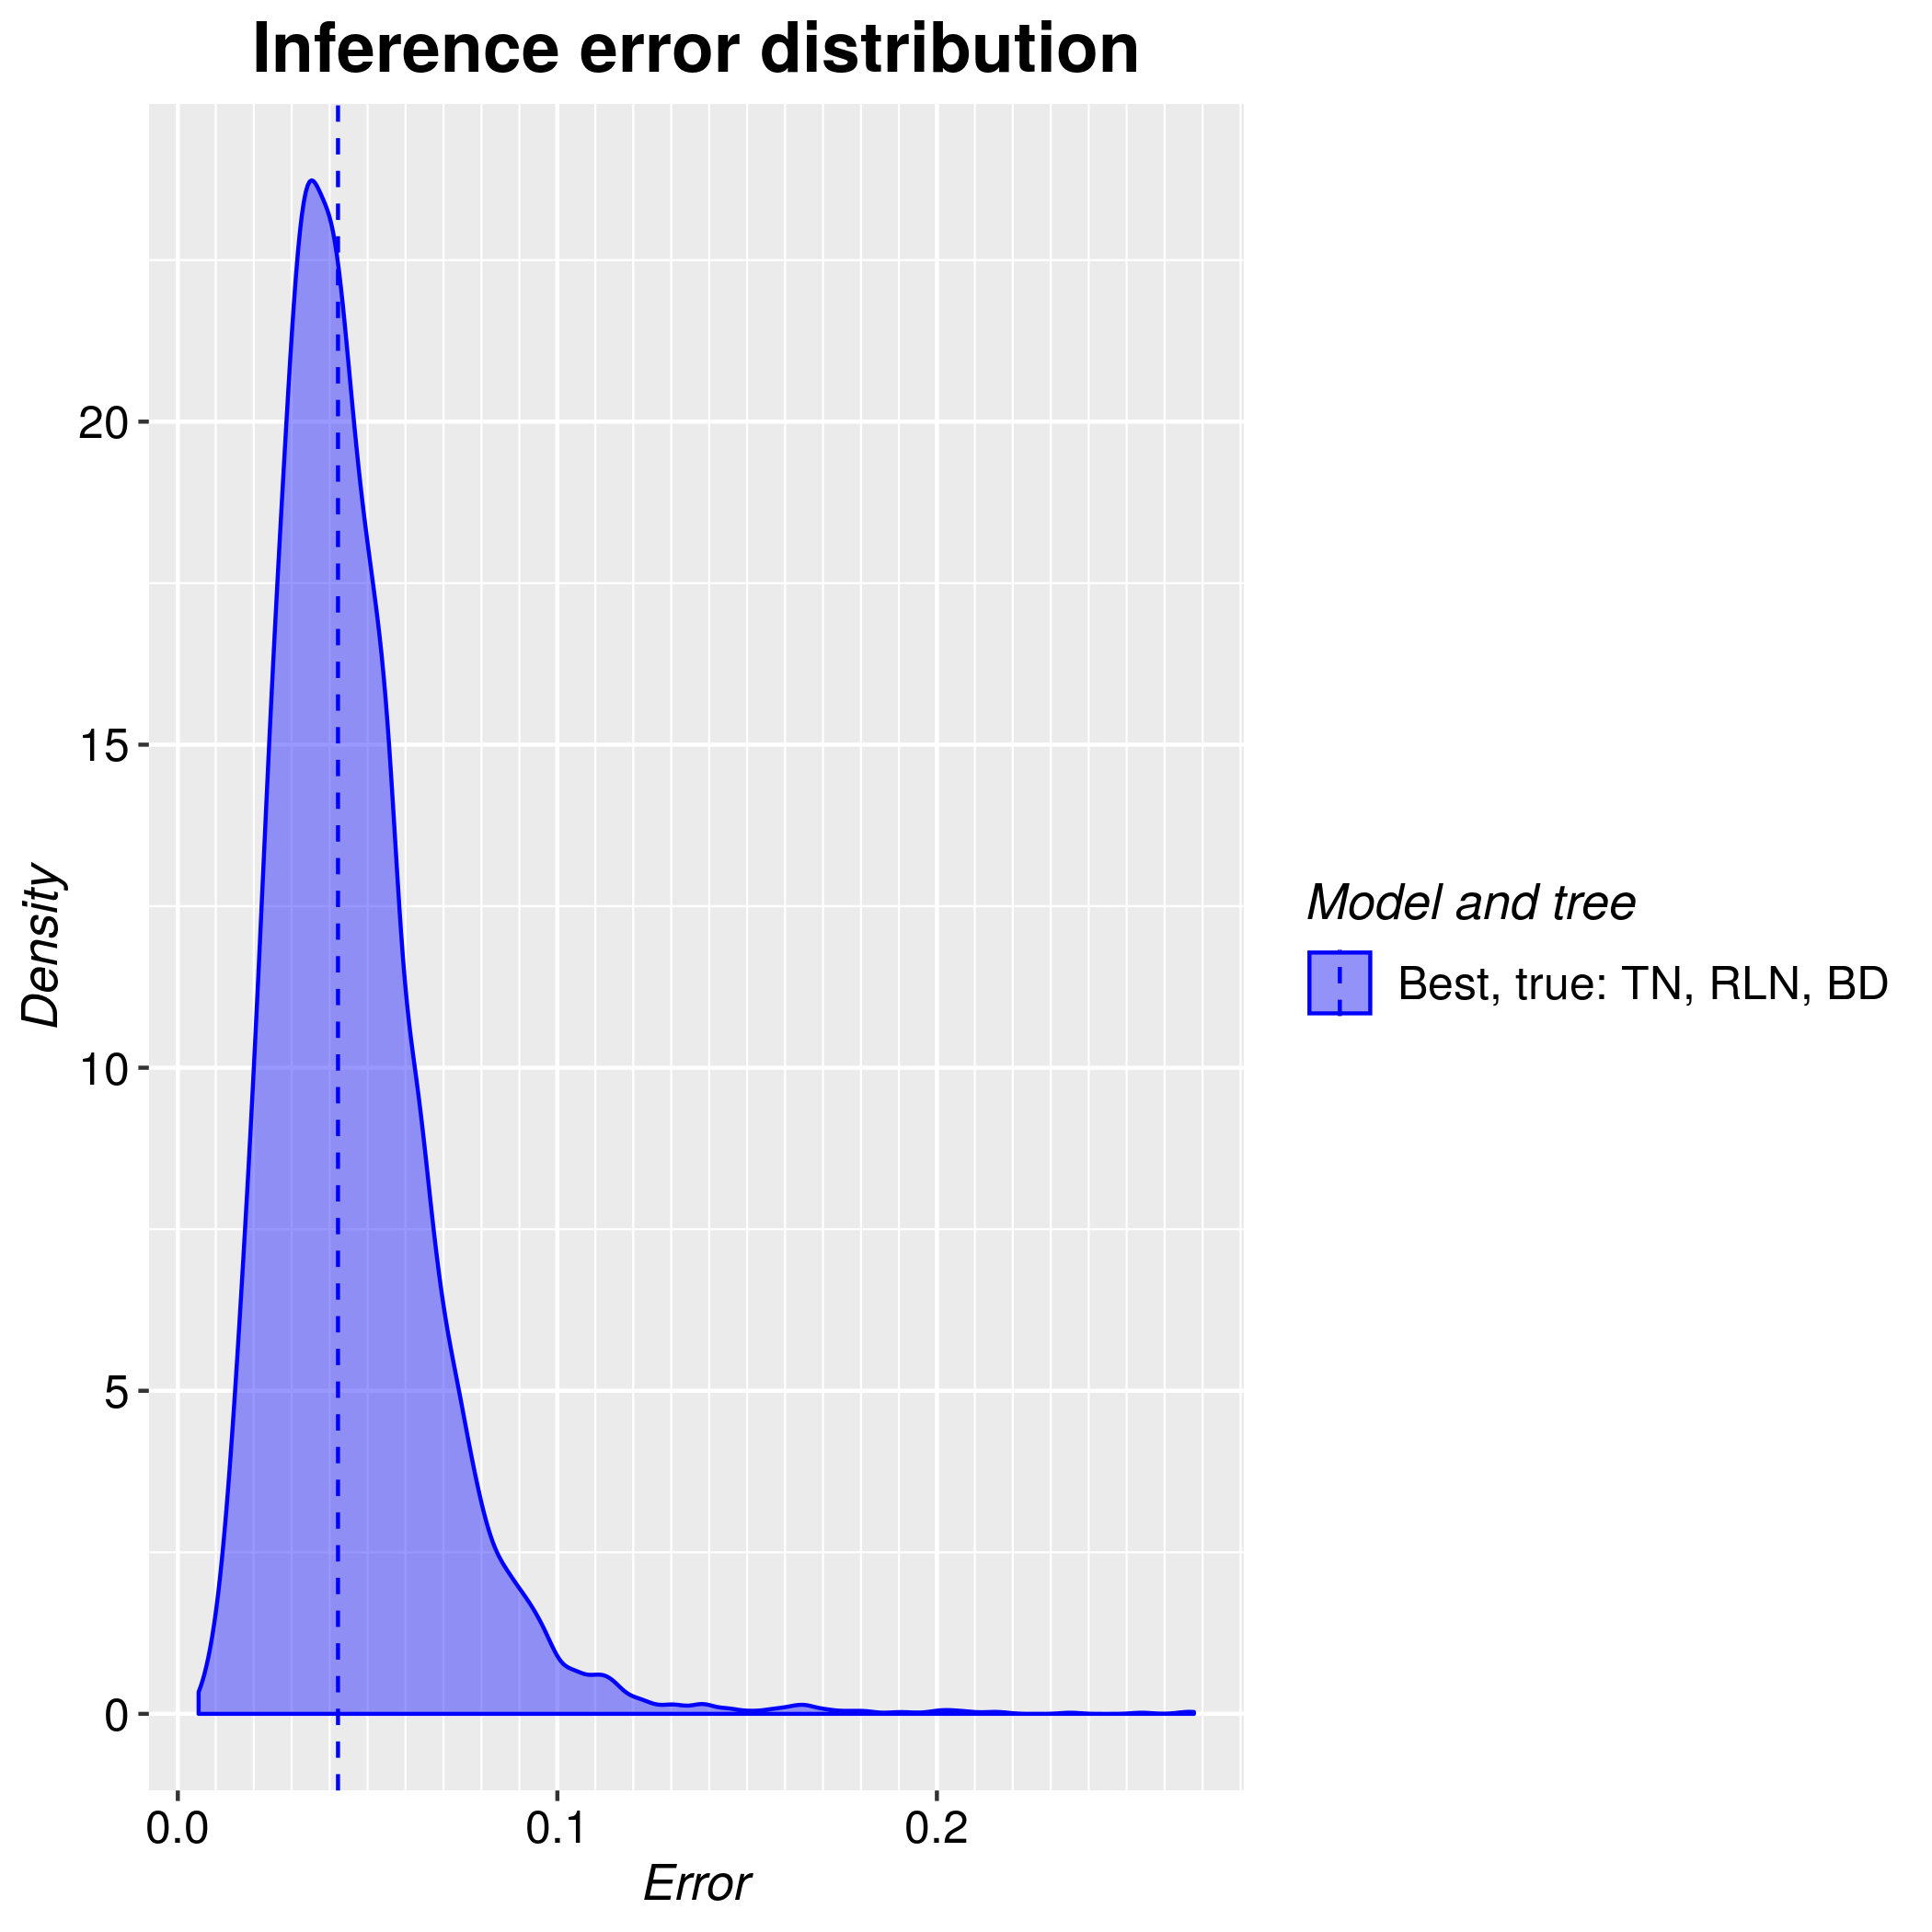
\includegraphics[width=\textwidth]{example_2/errors.png}
  \caption{
    Example 2: the error BEAST2 makes from a phylogeny when
    picking the best inference model.
  }
  \label{fig:example_2}
\end{figure}

%%%%%%%%%%%%%%%%%%%%%%%%%%%%%%%%%%%%%%%%%%%%%%%%%%%%%%%%%%%%%%%%%%%%%%%%%%%%%%%%
\section{Usage: Example Research Question 3}
%%%%%%%%%%%%%%%%%%%%%%%%%%%%%%%%%%%%%%%%%%%%%%%%%%%%%%%%%%%%%%%%%%%%%%%%%%%%%%%%

In ERQ 1 we measured the baseline error of the \verb;pirouette; method. We did so by using a standard tree prior to generate the original tree as well as in the inference.
The goal of \verb;pirouette; is to quantify the 
influence of a new (non-standard) tree prior.
To do so, we need to compare the inference error 
from the new tree prior to a baseline error,
by using a twin tree (see subsection~\ref{subsec:twinning}).
To do so, we use the twin tree as a control for the main pipeline.
In this example, we have no knowledge of the generative tree prior $\mathit{P}$
but we know the alignment model $\mathit{A}$.
In this ERQ it is reasonable to hand-pick a standard tree prior 
to serve as a stand-in generative tree prior as we assume that they are closely related.

\subsection{Question}

"What is the error made by BEAST2 from a phylogeny, 
when hand-picking a tree prior, compared to the background noise?"

\subsection{Answer}

Most of the settings for this ERQ are
the same as in the previous section. They are
the phylogeny from an unknown speciation model 
(listing~\ref{lst:unknown_phylogeny}), 
the alignment parameters (listing~\ref{lst:create_alignment})
and the list of experiments (listing~\ref{lst:create_generative_experiment}),
the latter stating that the generative tree prior is a Yule tree prior.

This time, however, we are interested in measuring both the inference error
and a baseline error. We do so by setting the twinning parameters $\mathit{T}$ to create a twin tree. A twin tree
has the same topology as the given tree, yet its branching times are simulated 
according to the standard tree prior used by BEAST2 to produce the posterior 
for the main pipeline. 
Since there is coherence between the inference model and the generative model, 
we expect BEAST2 to produce a posterior of phylogenies that are more similar to the 
original one, respect to the outcome of the main pipeline. 
Due to this, the twinning process is used to provide a control for the main 
experiment.

Creating the twinning parameters is easy, as it has sensible default settings.
For the sake of clarity, we explicitly show the default values of the most
important arguments:

\begin{lstlisting}[
  language=R, 
  floatplacement=ht, 
  frame=single,
  label = {lst:create_twinning_params},
  caption = Create the default twinning parameters
]
twinning_params <- create_twinning_params(
  twin_model = "bd", 
  method = "random_tree"
)
\end{lstlisting}

\richel{
  I would enjoy being able to write ...
}
\begin{lstlisting}
  twinning_params <- create_twinning_params(
    tree_prior = create_bd_tree_prior(),
    ...
  )
)
\end{lstlisting}
\richel{
  ... as that would connect the tree priors more
}

We bundle again all the \verb;pirouette; arguments using \verb;create_pir_params;:

\begin{lstlisting}[language=R, floatplacement=ht, frame=single]
pir_params <- create_pir_params(
  alignment_params = alignment_params,
  experiments = experiments,
  twinning_params = twinning_params
)
\end{lstlisting}

Finally, we run and plot the results:

\begin{lstlisting}[language=R, floatplacement=ht, frame=single]
errors <- pir_run(
  phylogeny = phylogeny,
  pir_params = pir_params
)
pir_plot(errors)
\end{lstlisting}

The output is shown in figure~\ref{fig:example_3}

\begin{figure}[ht]
  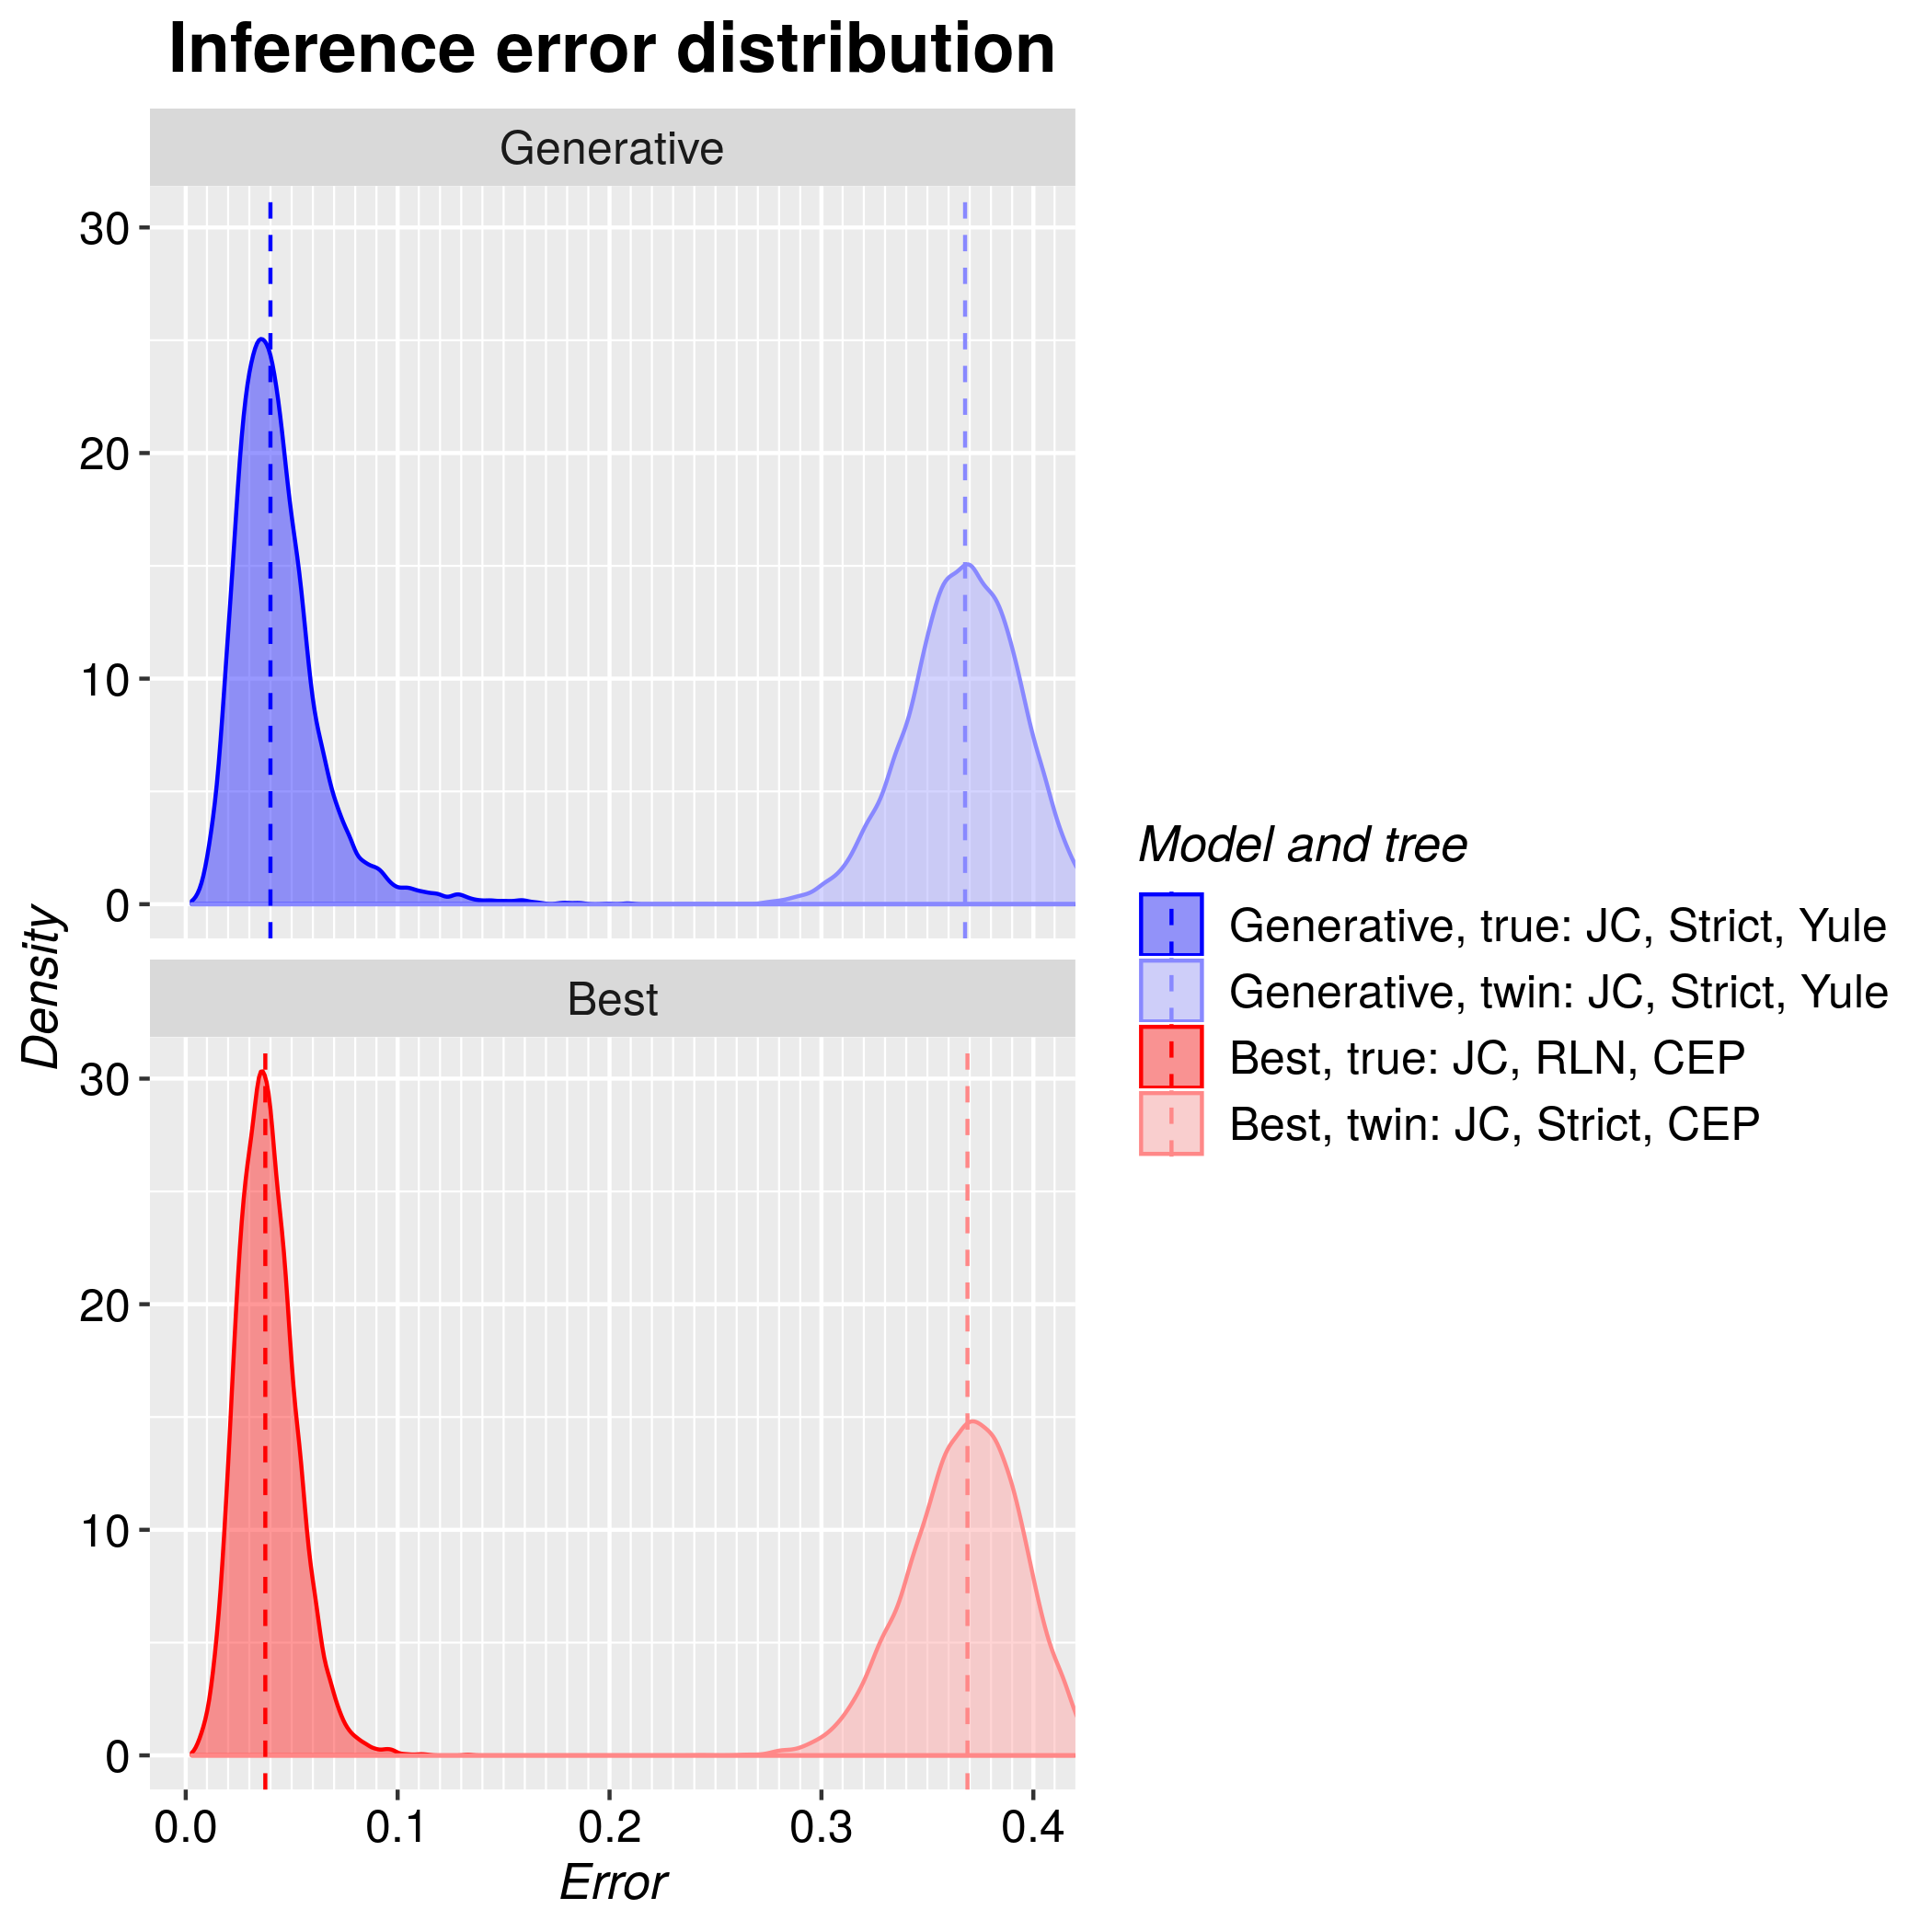
\includegraphics[width=\textwidth]{example_3/errors.png}
  \caption{
    Example 3: the error made by BEAST2 from a phylogeny, 
    when hand-picking a generative tree prior versus the control.
    Here, the 'twin' column shows the baseline inference error,
    as measured on the twin tree
  }
  \label{fig:example_3}
\end{figure}

%%%%%%%%%%%%%%%%%%%%%%%%%%%%%%%%%%%%%%%%%%%%%%%%%%%%%%%%%%%%%%%%%%%%%%%%%%%%%%%%
\section{Usage: Example Research Question 4}
%%%%%%%%%%%%%%%%%%%%%%%%%%%%%%%%%%%%%%%%%%%%%%%%%%%%%%%%%%%%%%%%%%%%%%%%%%%%%%%%

To answer ERQ 2 we used an evidence-based model selection procedure to obtain 
an 
error distribution.
However, it is unclear to what extent this error is due to the mismatch between 
the tree priors (from generative and inference models) or due to stochasticity. 
As mentioned in ERQ 1, \verb;pirouette; provides a tool to evaluate this, using 
the twinning process. We now apply it to the same pipeline followed in ERQ 2.

\subsection{Question}

"What is the error made by BEAST2 from a phylogeny 
derived from an unknown speciation model,
when selecting the best inference model, 
in relation to the background error?"

\subsection{Answer}

Here, as in examples 2 and 3, we start with the phylogeny 
generated by an unknown speciation model (listing~\ref{lst:unknown_phylogeny}). 
The first step in \verb;pirouette; is to simulate a DNA alignment 
from the given phylogeny, for which we will use the same code 
as shown in listing~\ref{lst:create_alignment}.

We specify that we want all 40 inference models to compete 
by calling \verb;create_all_experiments;,
as we previously did in listing~\ref{lst:create_all_experiments}.

We choose again to use the default error measurement setup,
as shown in listing~\ref{lst:create_error_measure_params}.

To get an idea of a baseline error made by BEAST2, 
we also make use of the twinning option by using the
default twinning parameters, as shown in 
listing~\ref{lst:create_twinning_params}.

\begin{lstlisting}[language=R, floatplacement=ht, frame=single]
pir_params <- create_pir_params(
  alignment_params = alignment_params,
  experiments = experiments,
  error_measure_params = error_measure_params,
  twinning_params = twinning_params
)
\end{lstlisting}
\richel{
  Refer to earlier listing for this call to \texttt{create\_pir\_params}
}

We run the experiment:

\begin{lstlisting}[language=R, floatplacement=ht, frame=single]
errors <- pir_run(
  phylogeny = phylogeny,
  pir_params = pir_params
)
\end{lstlisting}
\richel{
  Refer to earlier listing for this call to \texttt{pir\_run}
}

and show the results:

\begin{lstlisting}[language=R, floatplacement=ht, frame=single]
pir_plot(errors)
\end{lstlisting}
\richel{
  Refer to earlier listing for this call to \texttt{pir\_run}
}

The output is shown in figure~\ref{fig:example_4}.

\giovanni{describe winner}
\richel{agreed, after the figures also show it :-) }

\begin{figure}[ht]
  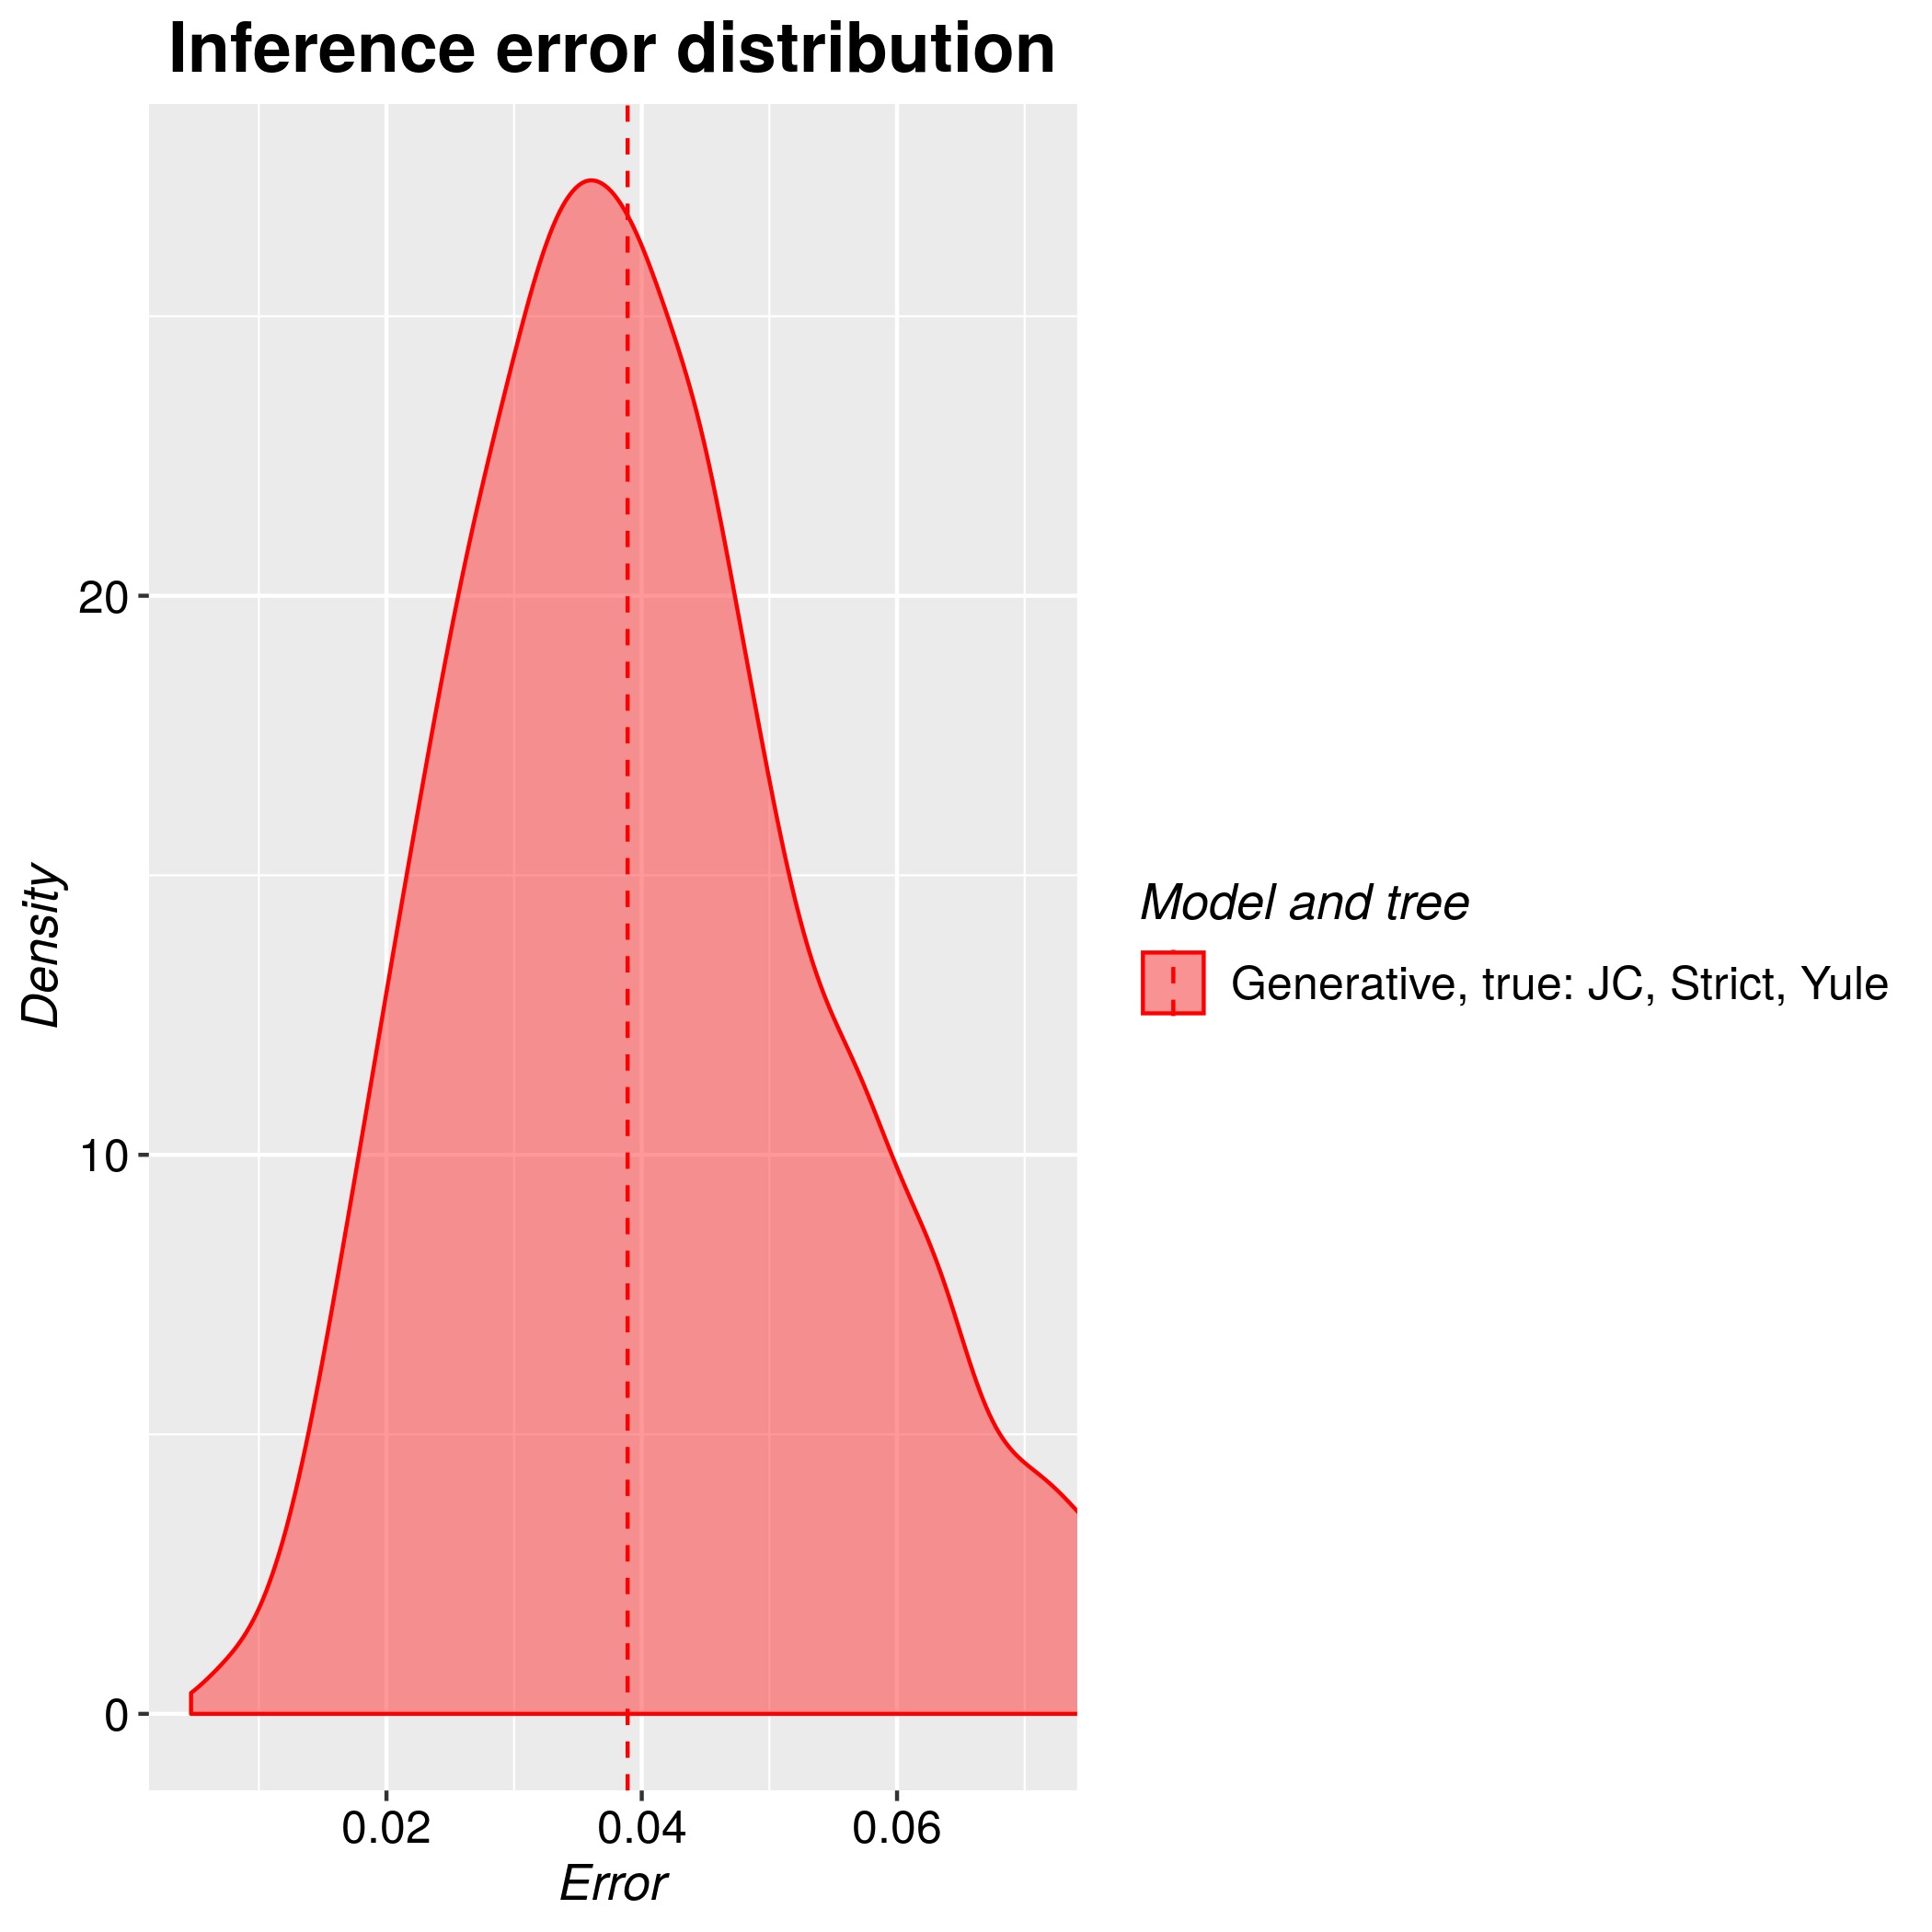
\includegraphics[width=\textwidth]{example_4/errors.png}
  \caption{
    Example 4: the error made by BEAST2 from a phylogeny, when the generative 
    model is known, compared to candidates with similar inference models, in 
    relationship to the background error.
  }
  \label{fig:example_4}
\end{figure}


%%%%%%%%%%%%%%%%%%%%%%%%%%%%%%%%%%%%%%%%%%%%%%%%%%%%%%%%%%%%%%%%%%%%%%%%%%%%%%%%
\section{Usage: Example Research Question 5}
%%%%%%%%%%%%%%%%%%%%%%%%%%%%%%%%%%%%%%%%%%%%%%%%%%%%%%%%%%%%%%%%%%%%%%%%%%%%%%%%

In ERQs 1 and 2 we used \verb;pirouette; to  
run the analysis on the main pipeline, either using a 'generative' or a 
'best\_candidate' inference model, resulting in one error distribution,
that does not mean much on its own.
In ERQs 3 and 4 we measured the baseline error caused by stochasticity,
by running a parallel twin pipeline. This yielded two error distributions:
the baseline error and the complete inference error.

\subsection{Question}

"What is the error made by BEAST2 from a phylogeny, 
when the generative model is hand-picked, 
compared to candidates with similar inference models, 
in relation to the background error?"

\subsection{Answer}

In this example, we use a tree generated by the Yule process.
Instead of using the common Yule tree as in example 1, we will use
a Yule tree of low (actually: zero) likelihood: 
the one as used in ERQs 2-4, by using the code shown 
in listing~\ref{lst:unknown_phylogeny}.
The first step in \verb;pirouette; is to simulate a DNA alignment 
from the given phylogeny, for which we will use the same code 
as shown in listing~\ref{lst:create_alignment}.

\begin{table}
  \begin{tabular}{ | c | c | c | l | }
    \hline
    \textbf{model type} & \textbf{run if} & \textbf{measure evidence} & 
\textbf{inference model} \\ 
    \hline
    generative & always         & yes & JC, strict, Yule \\
    candidate  & best candidate & yes & JC, strict, BD \\
    candidate  & best candidate & yes & JC, strict, CCP \\
    candidate  & best candidate & yes & JC, strict, CEP \\
    \hline
  \end{tabular}
  \caption{
    Experimental setup to answer the fourth research question.
    JC: Jukes-Cantor site model.
    strict: strict clock model.
    Yule: Yule (pure-birth) tree prior.
    BD: birth-death tree prior.
    CCP: coalescent constant-population tree prior.
    CEP: coalescent exponential-population tree prior.
  }
  \label{tab:experiment_5}
\end{table}

In the second step we state our experiments. 
In this example, we must both specify the generative and candidate experiments. 
Here we specify the generative model:

\begin{lstlisting}[language=R, floatplacement=H, frame=single]
generative_experiment <- create_experiment(
  inference_conditions = create_inference_conditions(
    model_type = "generative",
    run_if = "always",
    do_measure_evidence = TRUE
  )
  inference_model = create_inference_model(
    site_model = create_jc69_site_model(),
    clock_model = create_strict_clock_model(),
    tree_prior = create_yule_tree_prior()
  )
)
\end{lstlisting}

We can specify all the candidates simply by calling 
\verb;create_all_experiments; and excluding the generative inference model,
resulting in 39 candidate experiments:

\begin{lstlisting}[language=R, floatplacement=H, frame=single]
candidate_experiments <- create_all_experiments(
  exclude_model = generative_experiment$inference_model
)
\end{lstlisting}

We need to combine these experiments into one set of experiments:

\begin{lstlisting}[language=R, floatplacement=H, frame=single]
experiments <- c(list(generative_experiment), candidate_experiments)
\end{lstlisting}
\giovanni{Does this code actually work?}

We choose again to use the default error measurement parameters
as created in listing~\ref{lst:create_error_measure_params}
and combine this with the same twinning parameters 
as used in listing~\ref{lst:create_twinning_params}:

\begin{lstlisting}[language=R, floatplacement=H, frame=single]
pir_params <- create_pir_params(
  alignment_params = alignment_params,
  experiments = experiments,
  error_measure_params = error_measure_params,
  twinning_params = twinning_params
)
\end{lstlisting}

We run the experiment in the usual fashion:

\begin{lstlisting}[language=R, floatplacement=H, frame=single]
errors <- pir_run(
  phylogeny = phylogeny,
  pir_params = pir_params
)
\end{lstlisting}

We plot the results:

\begin{lstlisting}[language=R, floatplacement=H, frame=single]
pir_plot(errors)
\end{lstlisting}

The output is shown in figure~\ref{fig:example_5}.

\giovanni{describe winner}
\richel{agreed, after the figures also show it :-) }

\begin{figure}[ht]
  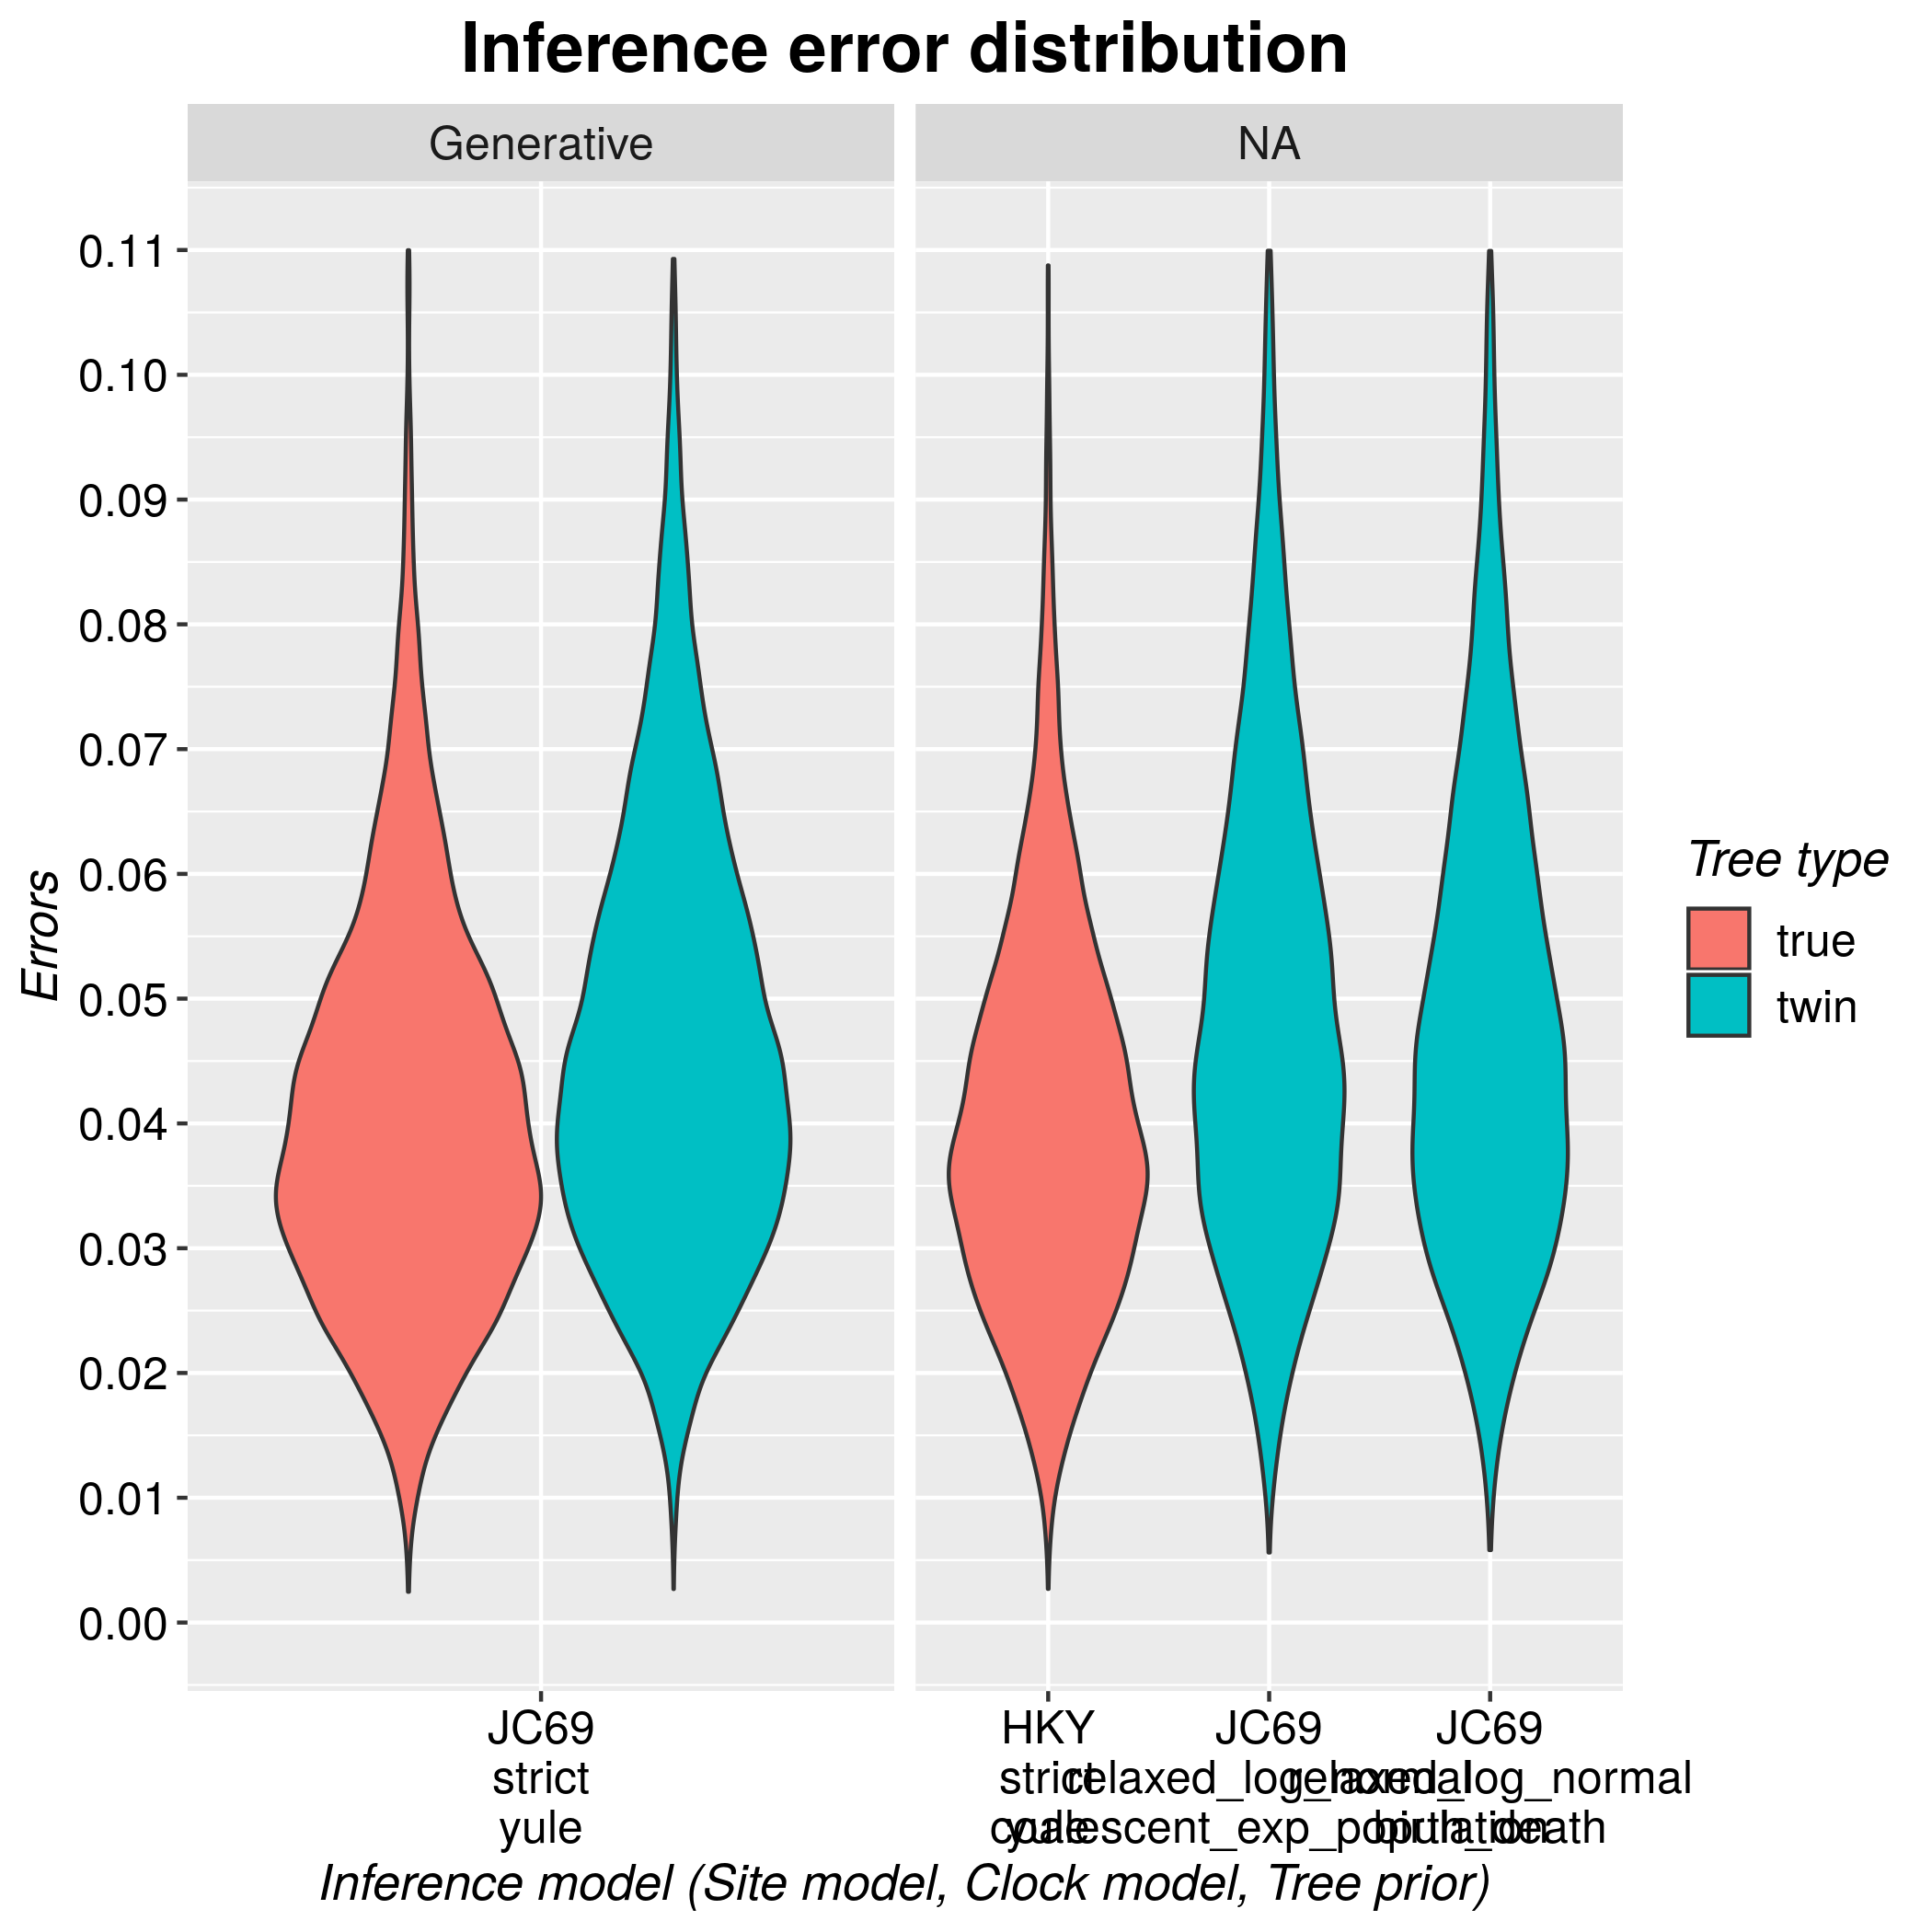
\includegraphics[width=\textwidth]{example_5/errors.png}
  \caption{
    Example 5: the error made by BEAST2 from a phylogeny, 
    when the generative model is known, 
    compared to candidates with similar inference models, 
    in relationship to the background error.
  }
  \label{fig:example_5}
\end{figure}

%%%%%%%%%%%%%%%%%%%%%%%%%%%%%%%%%%%%%%%%%%%%%%%%%%%%%%%%%%%%%%%%%%%%%%%%%%%%%%%%
\section{Interpretation}
%%%%%%%%%%%%%%%%%%%%%%%%%%%%%%%%%%%%%%%%%%%%%%%%%%%%%%%%%%%%%%%%%%%%%%%%%%%%%%%%

\richel{
  I think we can put the interpretation in a table as well.
  Question is: do you agree with the interpretations I gave?
  Please correct me.
}

\begin{table}
  \begin{tabular}{ | r | c | c | c | }
    \hline
    \textbf{Compare with} & \textbf{E2} & \textbf{E3} & \textbf{E4} \\ 
    \hline
    \textbf{E1} & Y & Y & N \\
    \textbf{E2} & . & N & Y \\
    \textbf{E3} & . & . & Y \\
    \textbf{E4} & . & . & . \\
    \hline
  \end{tabular}
  \caption{
    Error distributions that are relevant to compare.
    E1: true tree, generative model.
    E2: true tree, best candidate model.
    E3: true tree, generative model.
    E4: true tree, best candidate model.
    \giovanni{What if instead we use two letters, such as "TG", "TB", "WG", "WB"?}
    \giovanni{There is a typo: true tree is everywhere and twin is not present.}
  }
  \label{tab:relevant_comparisions}
\end{table}

\begin{table}
  \begin{tabular}{ | r | c | p{9cm} | }
    \hline
    \textbf{Condition} & \textbf{Expectation} & \textbf{Interpretation} \\ 
    \hline
    %%%%%%%%%%%%%%%%%%%%%%%%%%%%%%%%%%%%%%%%%%%%%%%%%%%%%%%%%%%%%%%%%%%%%%%%%%%%
    \textbf{$E1 > E2$}       & Unexpected & Novel tree prior is more related to 
      best candidate than hand-picked tree prior \\
    %%%%%%%%%%%%%%%%%%%%%%%%%%%%%%%%%%%%%%%%%%%%%%%%%%%%%%%%%%%%%%%%%%%%%%%%%%%%
    \textbf{$E1 \approx E2$} & Possible   & Hand-picked tree prior is just as 
      suitable as the best candidate tree prior \\
    %%%%%%%%%%%%%%%%%%%%%%%%%%%%%%%%%%%%%%%%%%%%%%%%%%%%%%%%%%%%%%%%%%%%%%%%%%%%
    \textbf{$E1 < E2$}       & Expected   & Hand-picked tree prior is the most 
      related tree prior \\
    %%%%%%%%%%%%%%%%%%%%%%%%%%%%%%%%%%%%%%%%%%%%%%%%%%%%%%%%%%%%%%%%%%%%%%%%%%%%
    \hline
    %%%%%%%%%%%%%%%%%%%%%%%%%%%%%%%%%%%%%%%%%%%%%%%%%%%%%%%%%%%%%%%%%%%%%%%%%%%%
    \textbf{$E1 > E3$}       & Unknown    & Novel tree prior important \\
    %%%%%%%%%%%%%%%%%%%%%%%%%%%%%%%%%%%%%%%%%%%%%%%%%%%%%%%%%%%%%%%%%%%%%%%%%%%%
    \textbf{$E1 \approx E3$} & Unknown    & Novel tree prior unimportant \\
    %%%%%%%%%%%%%%%%%%%%%%%%%%%%%%%%%%%%%%%%%%%%%%%%%%%%%%%%%%%%%%%%%%%%%%%%%%%%
    \textbf{$E1 < E3$}       & Unexpected & Twinning procedure increases 
      inference errors when using hand-picked tree prior \\
    %%%%%%%%%%%%%%%%%%%%%%%%%%%%%%%%%%%%%%%%%%%%%%%%%%%%%%%%%%%%%%%%%%%%%%%%%%%%
    \hline
    %%%%%%%%%%%%%%%%%%%%%%%%%%%%%%%%%%%%%%%%%%%%%%%%%%%%%%%%%%%%%%%%%%%%%%%%%%%%
    \textbf{$E2 > E4$}       & Expected   & Impact of novel tree prior cannot 
      be compensated for by model selection: twin tree with low likelihood? \\
    %%%%%%%%%%%%%%%%%%%%%%%%%%%%%%%%%%%%%%%%%%%%%%%%%%%%%%%%%%%%%%%%%%%%%%%%%%%%
    \textbf{$E2 \approx E4$} & Possible   & Best candidate tree priors perform 
      equally well in true and twin tree: true and twin tree similar? \\
    %%%%%%%%%%%%%%%%%%%%%%%%%%%%%%%%%%%%%%%%%%%%%%%%%%%%%%%%%%%%%%%%%%%%%%%%%%%%
    \textbf{$E2 < E4$}       & Unexpected & Twinning procedure increases 
      inference errors  when using best tree prior candidate \\
    %%%%%%%%%%%%%%%%%%%%%%%%%%%%%%%%%%%%%%%%%%%%%%%%%%%%%%%%%%%%%%%%%%%%%%%%%%%%
    \hline
    %%%%%%%%%%%%%%%%%%%%%%%%%%%%%%%%%%%%%%%%%%%%%%%%%%%%%%%%%%%%%%%%%%%%%%%%%%%%
    \textbf{$E3 > E4$}       & Unexpected & Hand-picked tree prior (that equals 
      the twinning tree prior!) worse than best candidate tree prior \\
    %%%%%%%%%%%%%%%%%%%%%%%%%%%%%%%%%%%%%%%%%%%%%%%%%%%%%%%%%%%%%%%%%%%%%%%%%%%%
    \textbf{$E3 \approx E4$} & Possible   & Twin tree fits equally well to the 
      hand-picked and best candidate tree prior  \\
    %%%%%%%%%%%%%%%%%%%%%%%%%%%%%%%%%%%%%%%%%%%%%%%%%%%%%%%%%%%%%%%%%%%%%%%%%%%%
    \textbf{$E3 < E4$}       & Expected   & Hand-pick tree prior (that equals 
      the twinning tree prior) performs as expected \\
    %%%%%%%%%%%%%%%%%%%%%%%%%%%%%%%%%%%%%%%%%%%%%%%%%%%%%%%%%%%%%%%%%%%%%%%%%%%%
    \hline
  \end{tabular}
  \caption{
    Interpretation of the different error distributions.
    This assumes that the operators ($<$, $\approx$ and $>$) to compare
    distributions are defined.
    E1: true tree, generative model.
    E2: true tree, best candidate model.
    E3: true tree, generative model.
    E4: true tree, best candidate model.
  }
  \label{tab:interpretation}
\end{table}


%%%%%%%%%%%%%%%%%%%%%%%%%%%%%%%%%%%%%%%%%%%%%%%%%%%%%%%%%%%%%%%%%%%%%%%%%%%%%%%%
\section{Discussion}
%%%%%%%%%%%%%%%%%%%%%%%%%%%%%%%%%%%%%%%%%%%%%%%%%%%%%%%%%%%%%%%%%%%%%%%%%%%%%%%%

In the five example research questions, 
we showed how to use \verb;pirouette; 
to quantify the importance of a tree prior in Bayesian phylogenetics.
In all ERQs we used and assumed the most simple tree prior possible,
which is the Yule tree prior.
In principle any other (more complex) generative tree prior 
can be tested, but we chose to provide the 
simplest (and fastest to run) examples.
All tests were performed on a single original tree, 
hence not providing us enough statistical power to 
evaluate the level of accuracy of the inference. 

However, if the same procedure were repeated and performed on a distribution 
with a sufficient number of generative trees, 
it could actually constitute a quantitative assessment 
of the quality of the inference.
To give an idea of the insights \verb;pirouette; can give,
we pretend the results of the example research questions
to be obtained from thousands of replicates.
In that case, figure~\ref{fig:example_1} shows 
the minimum error BEAST2 when the
generative model is known, which can serve as 
a minimum noise level assessment in a bigger experiment.  
Figure~\ref{fig:example_2} shows that 
the best candidate model gives an error distribution similar to the unknown 
tree prior,
hinting that the candidate model would be just as good in inference.
Figure~\ref{fig:example_3} shows that 
the twin model gives an error distribution similar to the unknown tree prior,
hinting that the shape of the phylogeny with unknown tree prior
does not effect the error made by BEAST2.
Figure~\ref{fig:example_4} shows that 
the twin model and best candidate model give 
an error distribution similar to the unknown tree prior,
hinting that the shape of the phylogeny with unknown tree prior
does not effect the error made by BEAST2, 
and that the candidate model would be just as good in inference.

In conclusion, \verb;pirouette; can directly show 
the comparison between the results obtained 
on a new generative prior as compared to the error BEAST2 
would make when operating on a tree generated 
under a known, right and existing tree prior (the twin tree).
From such results an user can estimate whether or not a new tree prior, 
tailored on the generative process, is needed. 
If this would indeed be the case, 
one could implement their own tree prior as a new module in BEAST2.

%%%%%%%%%%%%%%%%%%%%%%%%%%%%%%%%%%%%%%%%%%%%%%%%%%%%%%%%%%%%%%%%%%%%%%%%%%%%%%%%
\section{pirouette resources}
%%%%%%%%%%%%%%%%%%%%%%%%%%%%%%%%%%%%%%%%%%%%%%%%%%%%%%%%%%%%%%%%%%%%%%%%%%%%%%%%

\verb;pirouette; is free, libre and open source software available at 
\url{http://github.com/richelbilderbeek/pirouette},
licensed under the GNU General Public License version 3.
\verb;pirouette; depends on multiple packages, which are:
\richel{I think we can get rid of some dependencies, we just need to check}
\verb;ape; (\cite{APE}), 
\verb;babette; (\cite{bilderbeek2018babette}),
\verb;becosys; (\cite{becosys}),
\verb;DDD; (\cite{DDD}),
\verb;devtools; (\cite{devtools}),
\verb;geiger; (\cite{geiger}),
\verb;ggplot2; (\cite{ggplot2}),
\verb;knitr; (\cite{knitr}),
\verb;lintr; (\cite{lintr}),
\verb;mcbette; (\cite{mcbette}),
\verb;nLTT; (\cite{nLTT}),
\verb;PBD; (\cite{PBD}),
\verb;phangorn; (\cite{phangorn}),
\verb;phytools; (\cite{phytools}),
\verb;rappdirs; (\cite{rappdirs}),
\verb;rmarkdown; (\cite{rmarkdown}),
\verb;Rmpfr; (\cite{Rmpfr}),
\verb;stringr; (\cite{stringr}),
\verb;subplex; (\cite{subplex}),
\verb;TESS; (\cite{TESS}),
\verb;testit; (\cite{testit}), 
\verb;testthat; (\cite{testthat}) and
\verb;tidyr; (\cite{tidyr}).

\verb;pirouette;'s development takes place on GitHub,
\url{https://github.com/richelbilderbeek/pirouette},
which allows submitting bug reports, requesting features, 
or adding code. To ensure a high quality, \verb;pirouette; 
uses a continuous integration service, has a code coverage of 100\%
and enforces the most commonly used R style guide (\cite{style_guide}).

\verb;pirouette;'s is extensively documentated on its website,
its documentation and its vignettes.
The \verb;pirouette; website is a good starting point to learn
how to use \verb;pirouette;, as it links to tutorials and videos.
The \verb;pirouette; package documentation describes
all functions and liberally links to related functions.
All exported functions show a minimal example as part of their documentation.
The \verb;pirouette; vignette demonstrates extensively how 
to use \verb;pirouette; in a more lightly written way. 

%%%%%%%%%%%%%%%%%%%%%%%%%%%%%%%%%%%%%%%%%%%%%%%%%%%%%%%%%%%%%%%%%%%%%%%%%%%%%%%%
\section{Citation of pirouette}
%%%%%%%%%%%%%%%%%%%%%%%%%%%%%%%%%%%%%%%%%%%%%%%%%%%%%%%%%%%%%%%%%%%%%%%%%%%%%%%%

Professionals using \verb;pirouette; can cite this
article. To obtain the citation from within R, use:

\begin{lstlisting}[language=R]
> citation("pirouette")
\end{lstlisting}

%%%%%%%%%%%%%%%%%%%%%%%%%%%%%%%%%%%%%%%%%%%%%%%%%%%%%%%%%%%%%%%%%%%%%%%%%%%%%%%%
\section{Acknowledgements}
%%%%%%%%%%%%%%%%%%%%%%%%%%%%%%%%%%%%%%%%%%%%%%%%%%%%%%%%%%%%%%%%%%%%%%%%%%%%%%%%

We would like to thank the Center for Information Technology of the University 
of Groningen for their support and for providing access to the Peregrine 
high performance computing cluster. 
We thank the Netherlands 
Organization for Scientific Research (NWO) for financial support 
through a VICI grant awarded to RSE.

%%%%%%%%%%%%%%%%%%%%%%%%%%%%%%%%%%%%%%%%%%%%%%%%%%%%%%%%%%%%%%%%%%%%%%%%%%%%%%%%
\section{Data Accessibility}
%%%%%%%%%%%%%%%%%%%%%%%%%%%%%%%%%%%%%%%%%%%%%%%%%%%%%%%%%%%%%%%%%%%%%%%%%%%%%%%%

All code is archived at 
\url{http://github.com/richelbilderbeek/pirouette_article},
with DOI \url{https://doi.org/12.3456/zenodo.1234567}.

%%%%%%%%%%%%%%%%%%%%%%%%%%%%%%%%%%%%%%%%%%%%%%%%%%%%%%%%%%%%%%%%%%%%%%%%%%%%%%%%
\section{Authors' contributions}
%%%%%%%%%%%%%%%%%%%%%%%%%%%%%%%%%%%%%%%%%%%%%%%%%%%%%%%%%%%%%%%%%%%%%%%%%%%%%%%%

RJCB, GL and RSE conceived the idea for the package. 
RJCB created and tested the package, and wrote the first draft of the 
manuscript.
GL tested the package and contributed substantially to revisions.
RSE contributed to revisions.

%%%%%%%%%%%%%%%%%%%%%%%%%%%%%%%%%%%%%%%%%%%%%%%%%%%%%%%%%%%%%%%%%%%%%%%%%%%%%%%%
% Bibliography
%%%%%%%%%%%%%%%%%%%%%%%%%%%%%%%%%%%%%%%%%%%%%%%%%%%%%%%%%%%%%%%%%%%%%%%%%%%%%%%%
% MEE style
\bibliographystyle{mee}
\bibliography{article}
%%%%%%%%%%%%%%%%%%%%%%%%%%%%%%%%%%%%%%%%%%%%%%%%%%%%%%%%%%%%%%%%%%%%%%%%%%%%%%%%

\appendix

%%%%%%%%%%%%%%%%%%%%%%%%%%%%%%%%%%%%%%%%%%%%%%%%%%%%%%%%%%%%%%%%%%%%%%%%%%%%%%%%
\section{Results in detail}
%%%%%%%%%%%%%%%%%%%%%%%%%%%%%%%%%%%%%%%%%%%%%%%%%%%%%%%%%%%%%%%%%%%%%%%%%%%%%%%%

%%%%%%%%%%%%%%%%%%%%%%%%%%%%%%%%%%%%%%%%%%%%%%%%%%%%%%%%%%%%%%%%%%%%%%%%%%%%%%%%
\subsection{Errors}
%%%%%%%%%%%%%%%%%%%%%%%%%%%%%%%%%%%%%%%%%%%%%%%%%%%%%%%%%%%%%%%%%%%%%%%%%%%%%%%%

%%%%%%%%%%%%%%%%%%%%%%%%%%%%%%%%%%%%%%%%%%%%%%%%%%%%%%%%%%%%%%%%%%%%%%%%%%%%%%%%
\subsection{Example 1}
%%%%%%%%%%%%%%%%%%%%%%%%%%%%%%%%%%%%%%%%%%%%%%%%%%%%%%%%%%%%%%%%%%%%%%%%%%%%%%%%

%%%%%%%%%%%%%%%%%%%%%%%%%%%%%%%%%%%%%%%%%%%%%%%%%%%%%%%%%%%%%%%%%%%%%%%%%%%%%%%%
\begin{figure}[ht]
  \centering
  \resizebox {0.8\columnwidth} {!} {
    \begin{tikzpicture}[
      ->,>=stealth',shorten >=1pt,auto,
      node distance=0.25\textheight, 
      semithick
    ]   
    \tikzstyle{every state}=[]
    \node[state, draw=none] (O) [] {
    };   
    \node[state] (A) [right of = O, rectangle] {
      \includegraphics[height=0.2\textheight]{example_1/true_tree.png}
    };   
    \node[state] (B) [below of = A, rectangle] {
      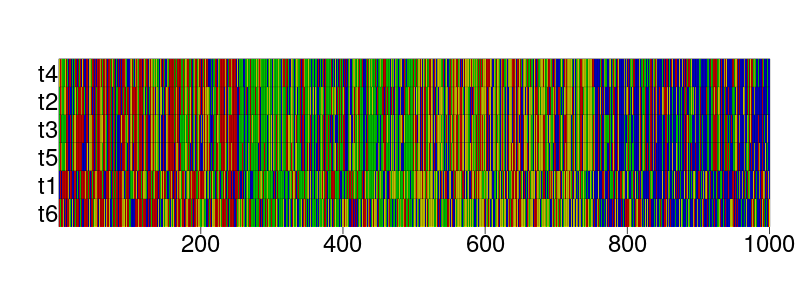
\includegraphics[height=0.2\textheight]{example_1/true_alignment.png}
    };   
    \node[state] (C) [below of = B, rectangle] {
      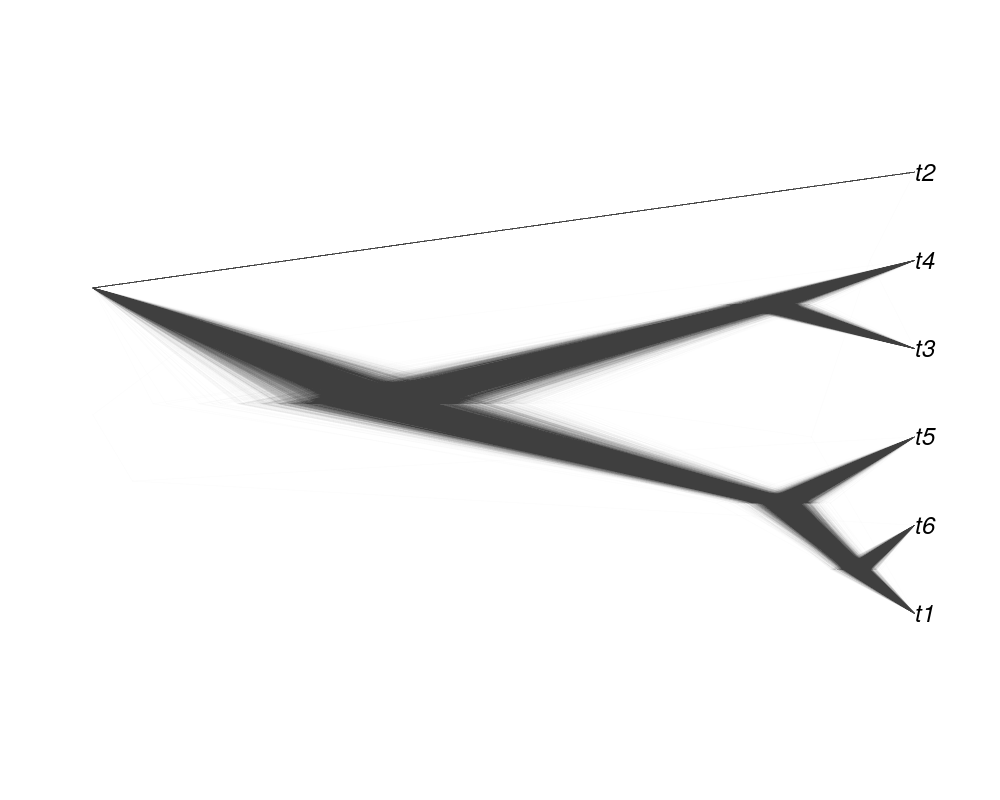
\includegraphics[height=0.2\textheight]{example_1/true_posterior_gen.png}
    };   
    \node[state] (D) [below of = C, rectangle] {
      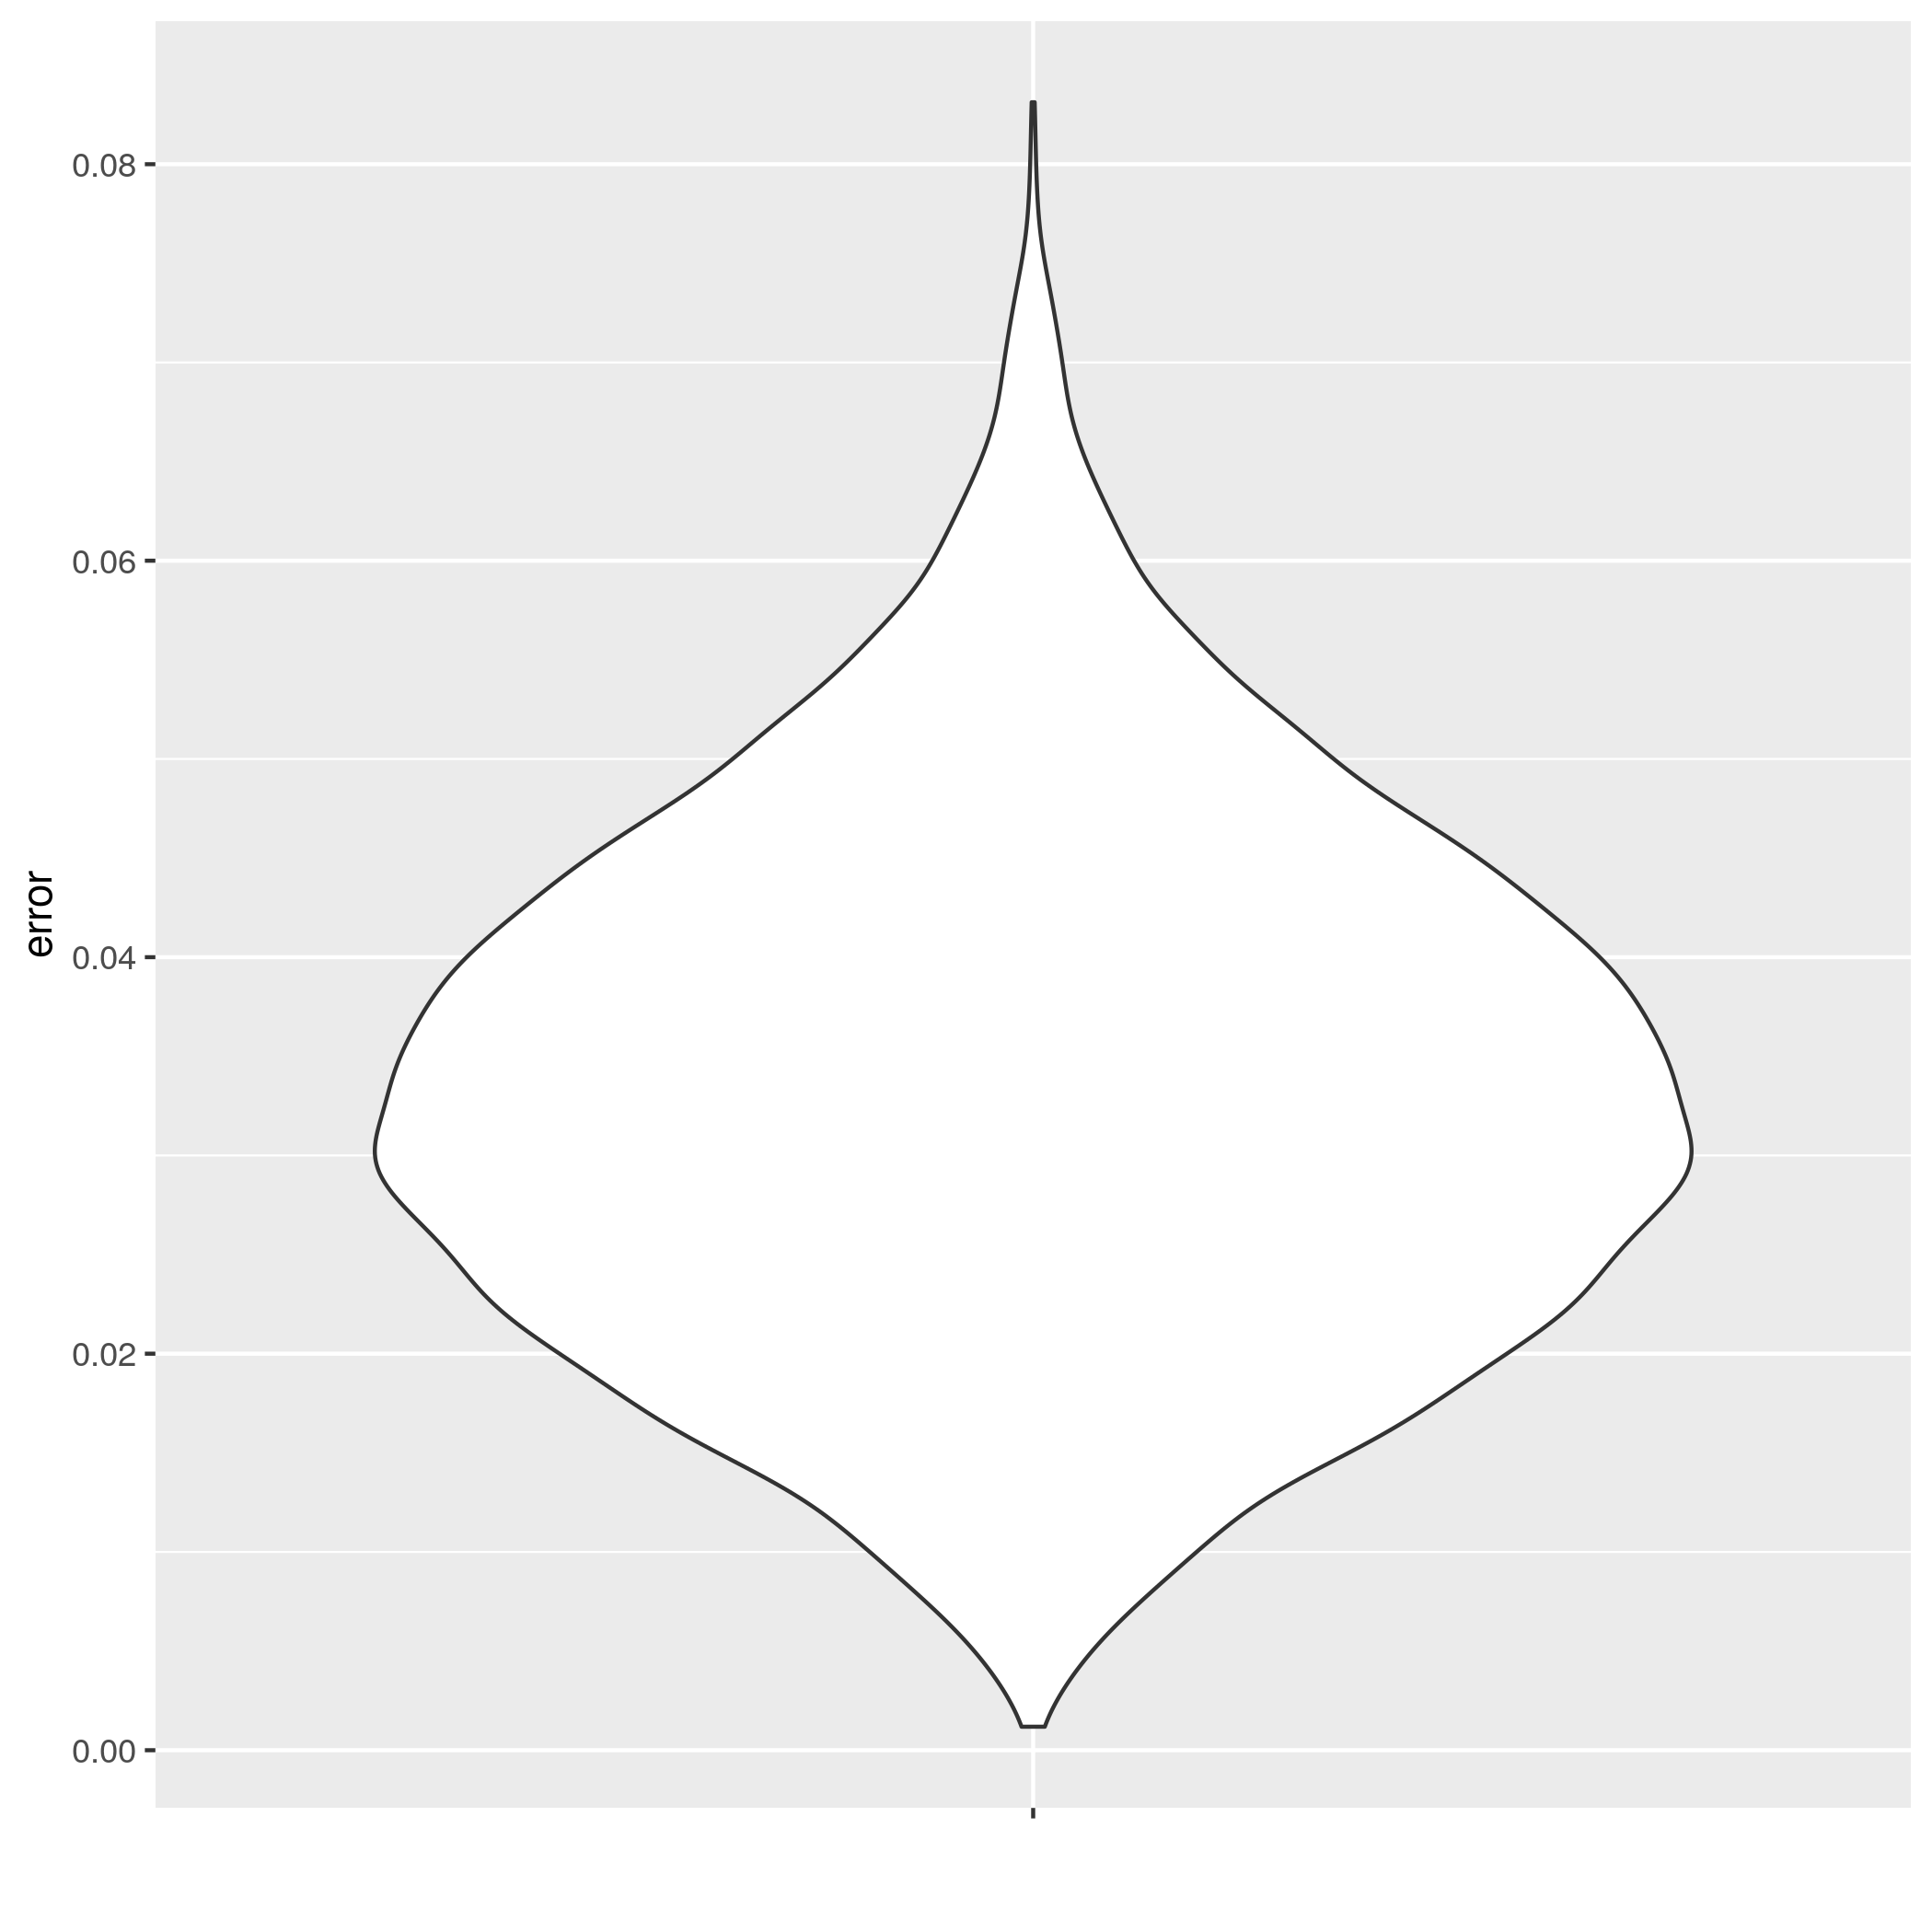
\includegraphics[height=0.2\textheight]{example_1/true_error_violin_gen.png}
    };   
    \path 
      (O) edge [anchor = south] node {} (A)
      (A) edge [anchor = south] node {} (B)
      (B) edge [anchor = south] node {} (C)
      (C) edge [anchor = south] node {} (D)
    ; 
    \end{tikzpicture}
  }
  \label{fig:example_1_full_pipeline}
  \caption{Example 1: full pipeline}
\end{figure}
%%%%%%%%%%%%%%%%%%%%%%%%%%%%%%%%%%%%%%%%%%%%%%%%%%%%%%%%%%%%%%%%%%%%%%%%%%%%%%%%

%%%%%%%%%%%%%%%%%%%%%%%%%%%%%%%%%%%%%%%%%%%%%%%%%%%%%%%%%%%%%%%%%%%%%%%%%%%%%%%%

\input{example_1/esses.latex}
% has label tab:esses_example_1

%%%%%%%%%%%%%%%%%%%%%%%%%%%%%%%%%%%%%%%%%%%%%%%%%%%%%%%%%%%%%%%%%%%%%%%%%%%%%%%%
\subsection{Example 2}
%%%%%%%%%%%%%%%%%%%%%%%%%%%%%%%%%%%%%%%%%%%%%%%%%%%%%%%%%%%%%%%%%%%%%%%%%%%%%%%%

%%%%%%%%%%%%%%%%%%%%%%%%%%%%%%%%%%%%%%%%%%%%%%%%%%%%%%%%%%%%%%%%%%%%%%%%%%%%%%%%
\begin{figure}[ht]
  \centering
  \resizebox {0.8\columnwidth} {!} {
    \begin{tikzpicture}[
      ->,>=stealth',shorten >=1pt,auto,
      node distance=0.25\textheight, 
      semithick
    ]   
    \tikzstyle{every state}=[]
    \node[state, draw=none] (O) [] {
    };   
    \node[state] (A) [right of = O, rectangle] {
      \includegraphics[height=0.2\textheight]{example_2/true_tree.png}
    };   
    \node[state] (B) [below of = A, rectangle] {
      \includegraphics[height=0.2\textheight]{example_2/true_alignment.png}
    };   
    \node[state] (C) [below of = B, rectangle] {
      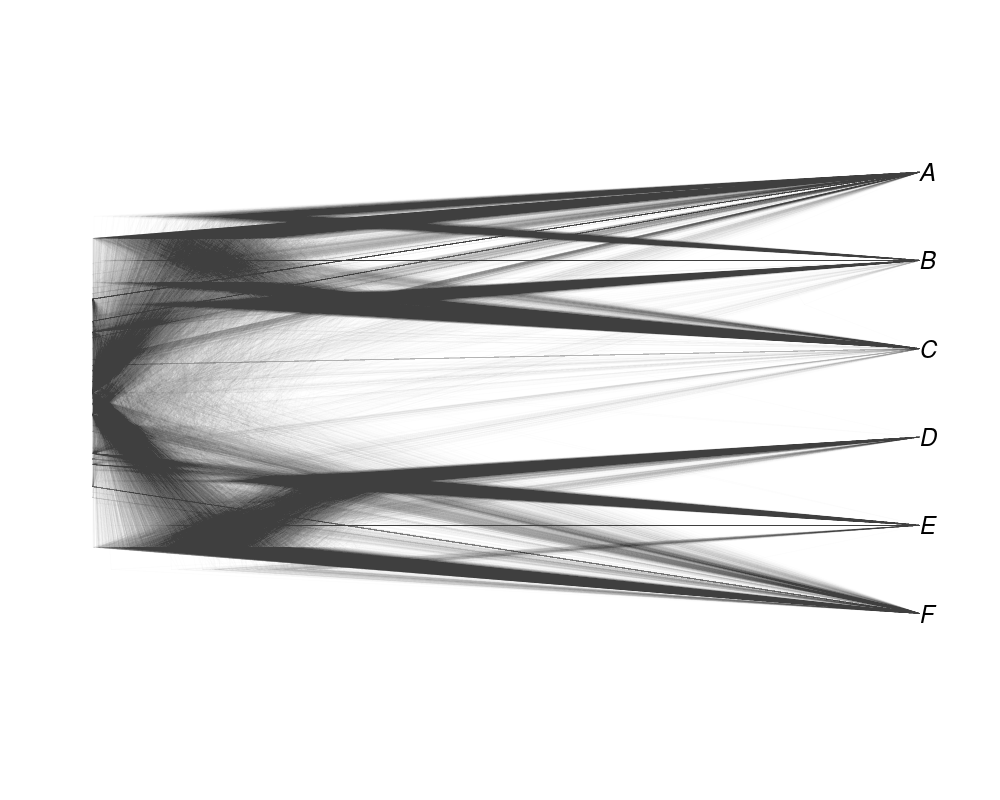
\includegraphics[height=0.2\textheight]{example_2/true_posterior_best.png}
    };   
    \node[state] (D) [below of = C, rectangle] {
      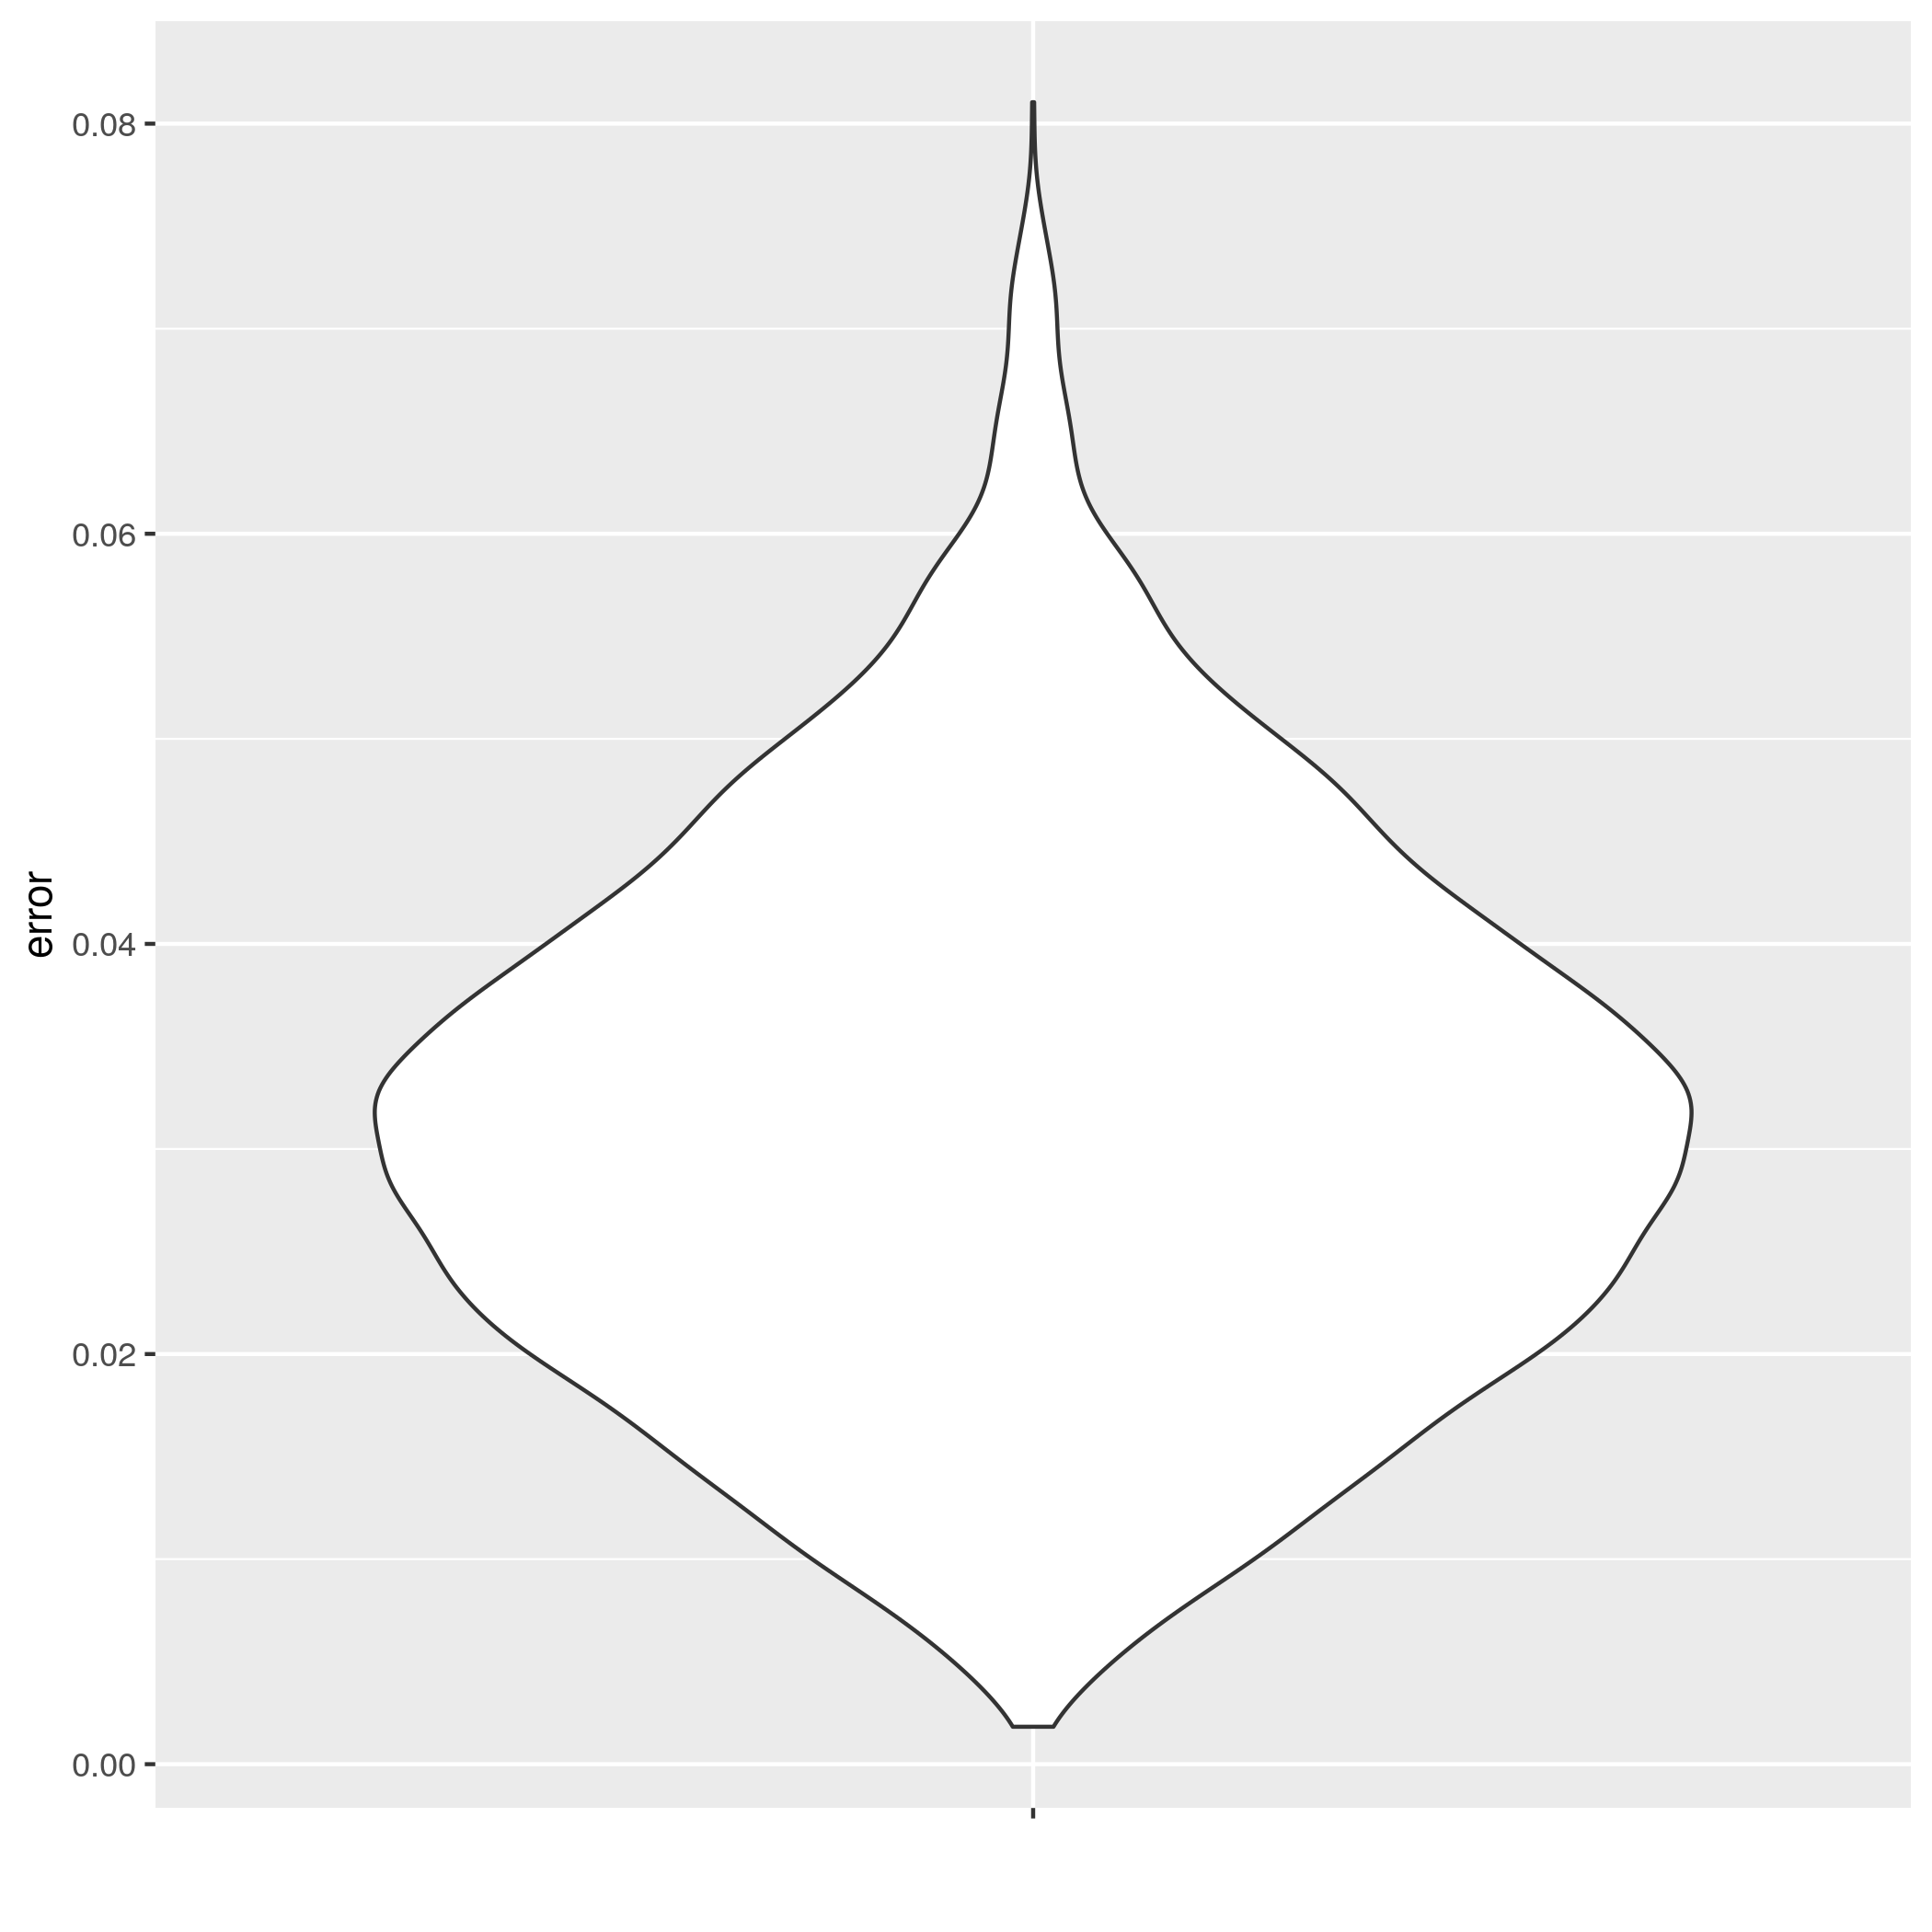
\includegraphics[height=0.2\textheight]{example_2/true_error_violin_best.png}
    };   
    \path 
      (O) edge [anchor = south] node {} (A)
      (A) edge [anchor = south] node {} (B)
      (B) edge [anchor = south] node {} (C)
      (C) edge [anchor = south] node {} (D)
    ; 
    \end{tikzpicture}
  }
  \label{fig:example_2_full_pipeline}
  \caption{Example 2: full pipeline}
\end{figure}
%%%%%%%%%%%%%%%%%%%%%%%%%%%%%%%%%%%%%%%%%%%%%%%%%%%%%%%%%%%%%%%%%%%%%%%%%%%%%%%%

\input{example_2/esses.latex}
% has label tab:esses_example_2

\input{example_2/evidences.latex}
% has label tab:evidences_example_2

%%%%%%%%%%%%%%%%%%%%%%%%%%%%%%%%%%%%%%%%%%%%%%%%%%%%%%%%%%%%%%%%%%%%%%%%%%%%%%%%
\subsection{Example 3}
%%%%%%%%%%%%%%%%%%%%%%%%%%%%%%%%%%%%%%%%%%%%%%%%%%%%%%%%%%%%%%%%%%%%%%%%%%%%%%%%

%%%%%%%%%%%%%%%%%%%%%%%%%%%%%%%%%%%%%%%%%%%%%%%%%%%%%%%%%%%%%%%%%%%%%%%%%%%%%%%%
\begin{figure}[ht]
  \centering
  \resizebox {0.8\columnwidth} {!} {
    \begin{tikzpicture}[
      ->,>=stealth',shorten >=1pt,auto,
      node distance=0.4\textheight, 
      semithick
    ]   
    \tikzstyle{every state}=[]
    \node[state, draw=none] (O) [] {
    };   
    \node[state] (A) [right of = O, rectangle] {
      \includegraphics[height=0.2\textheight]{example_3/true_tree.png}
    };   
    \node[state] (B) [below of = A, rectangle] {
      \includegraphics[height=0.13\textheight]{example_3/true_alignment.png}
    };   
    \node[state] (C) [below of = B, rectangle] {
      
\includegraphics[height=0.2\textheight]{example_3/true_posterior_gen.png}
    };   
    \node[state] (D) [below of = C, rectangle] {
      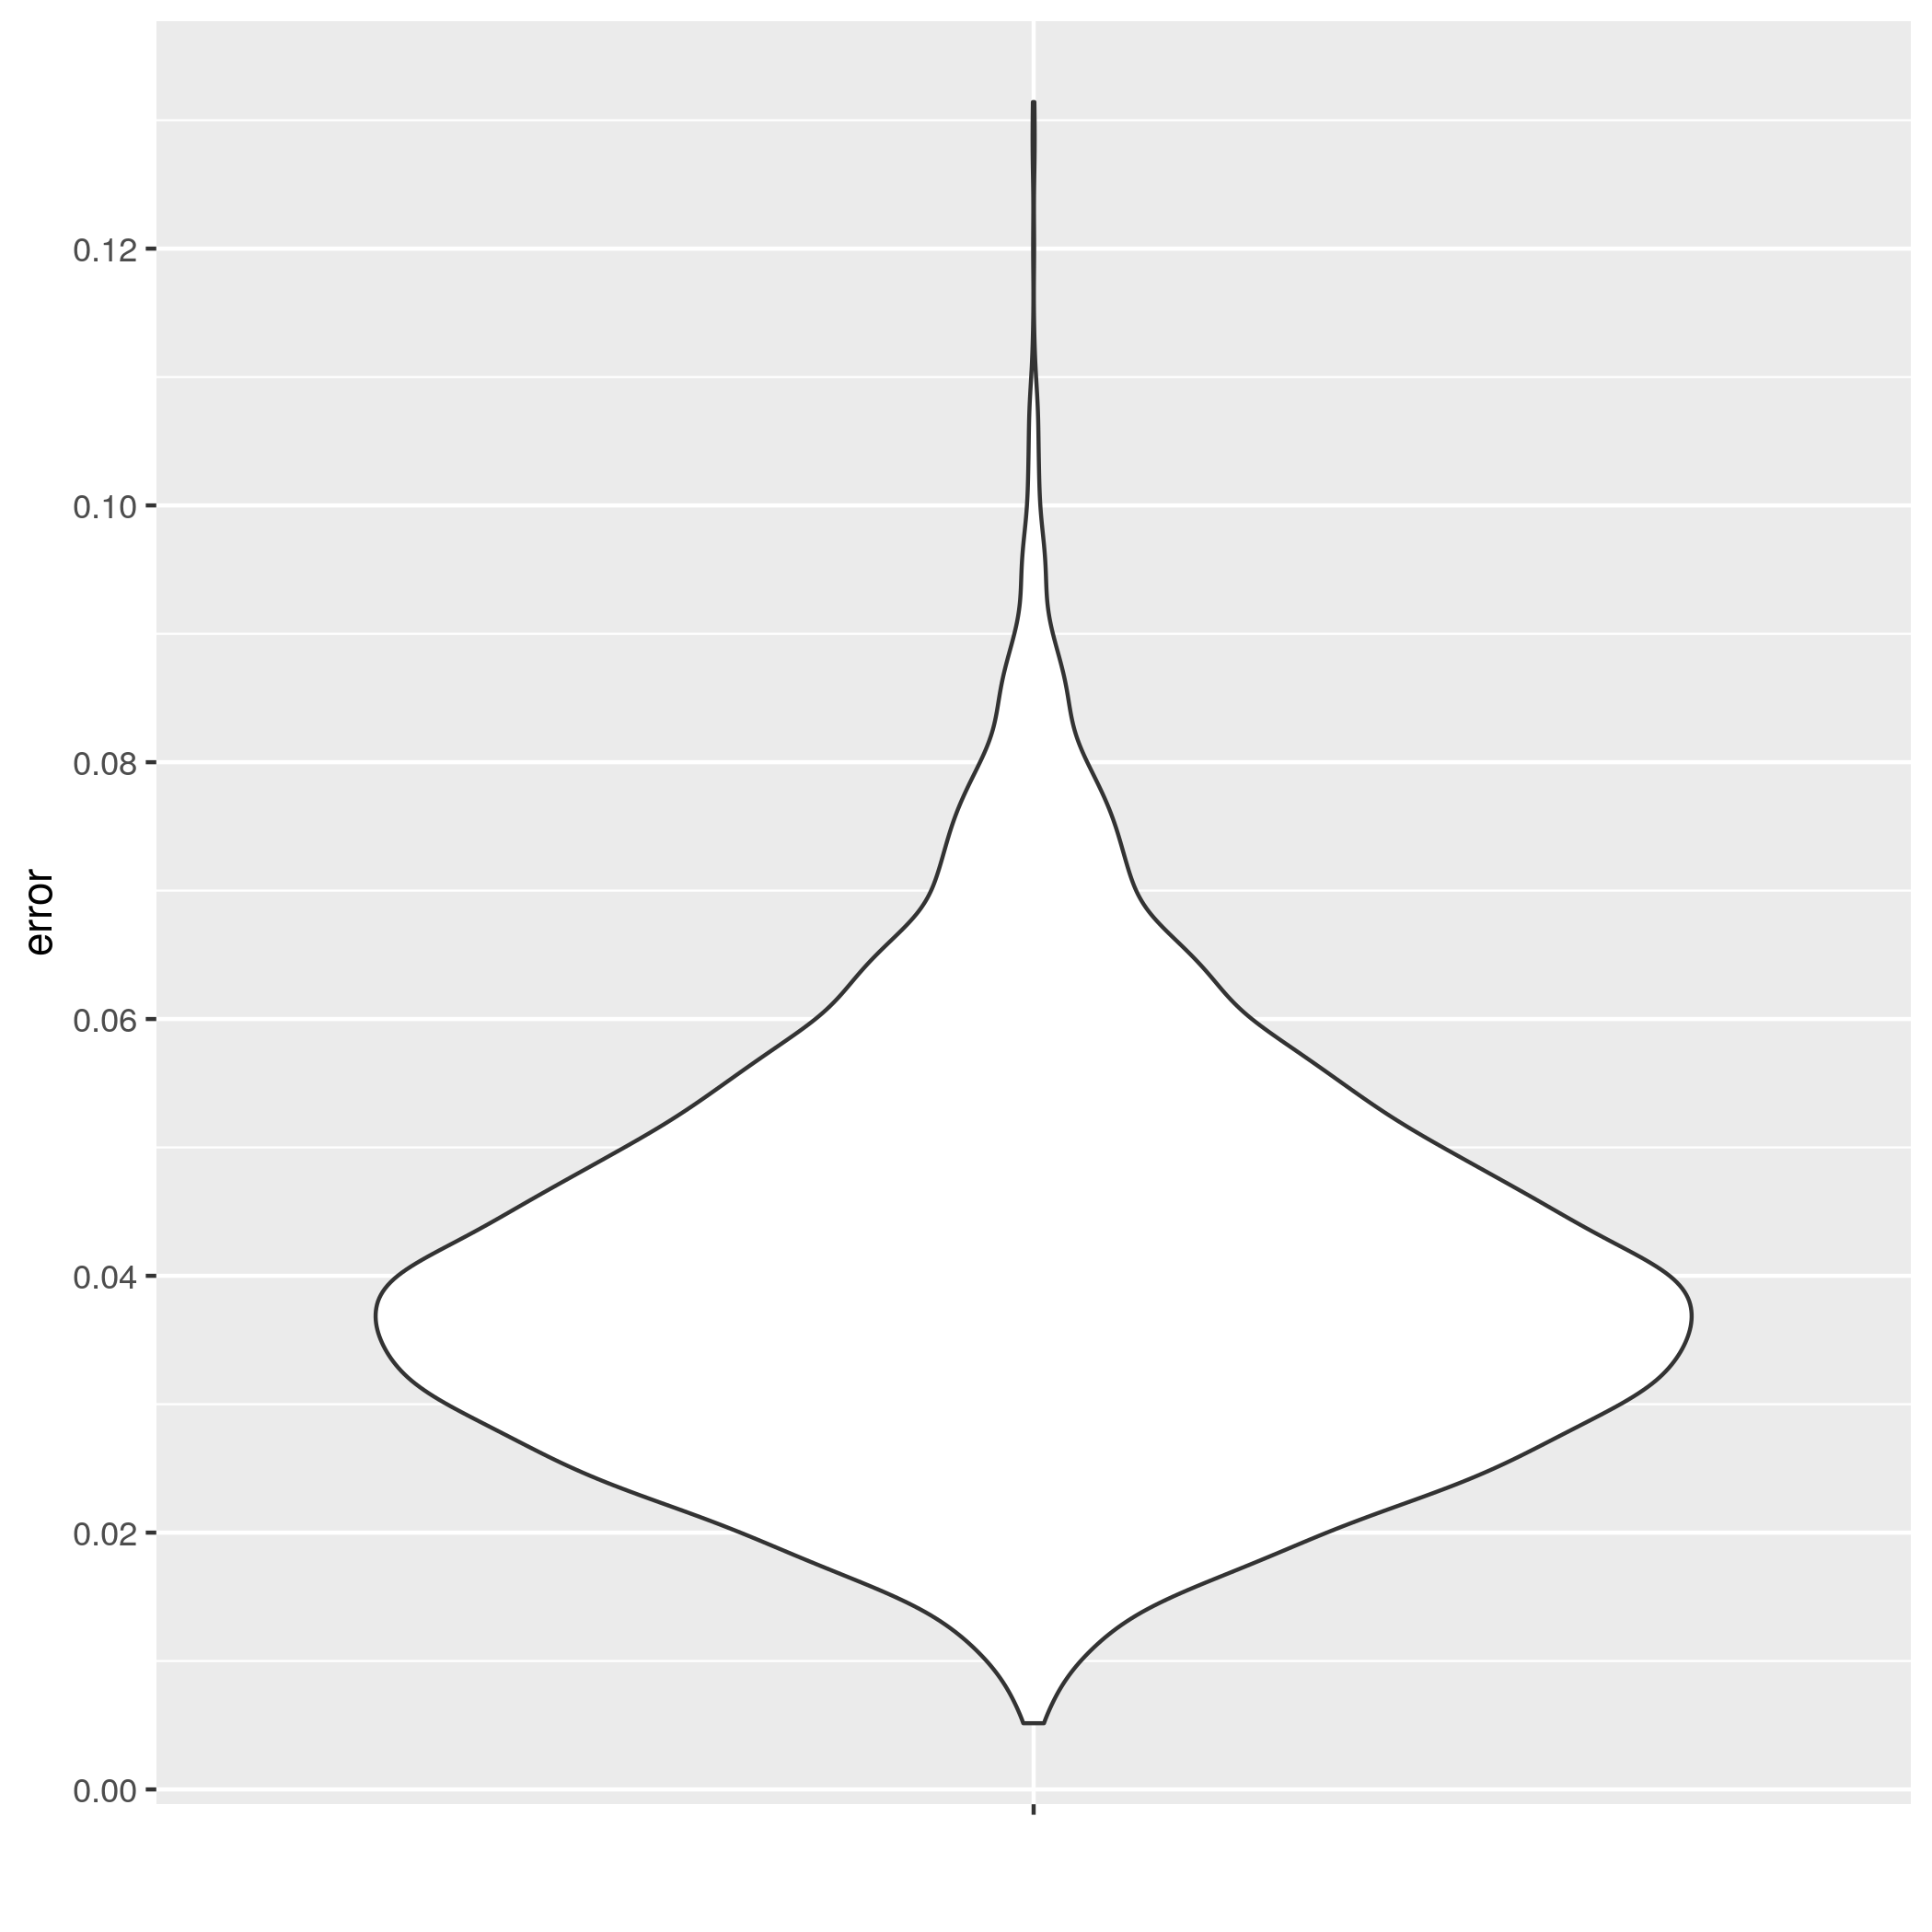
\includegraphics[height=0.2\textheight]{example_3/true_error_violin_gen.png}
    };   
    \node[state] (AT) [right of = A, rectangle] {
      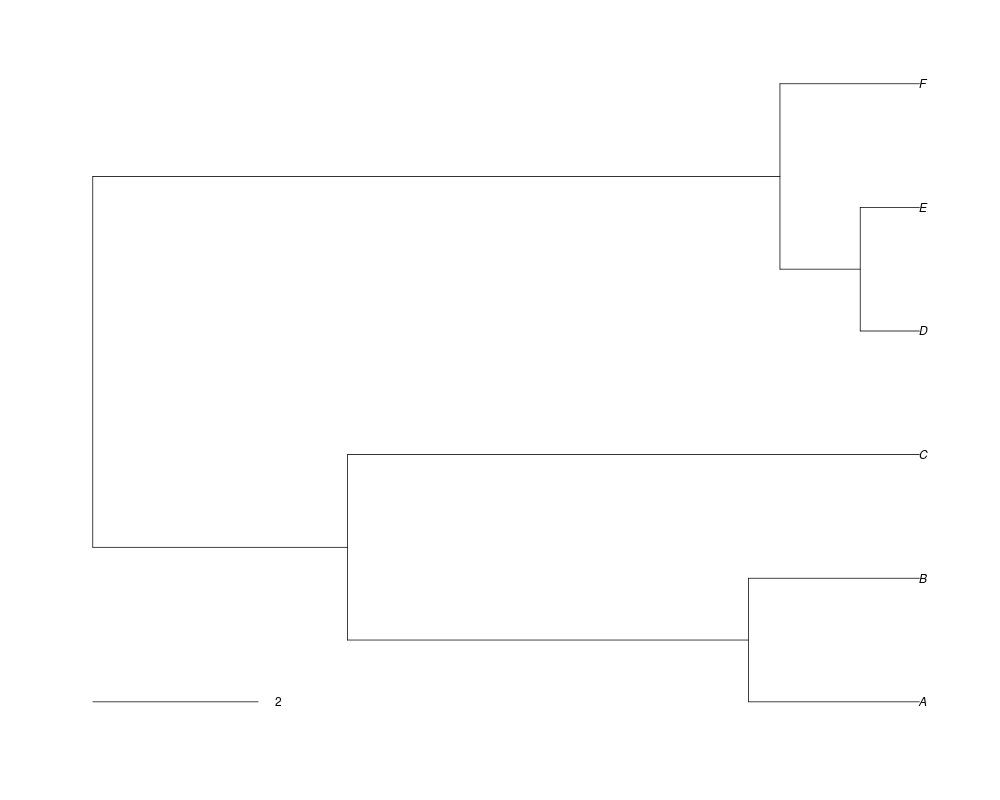
\includegraphics[height=0.2\textheight]{example_3/twin_tree.png}
    };   
    \node[state] (BT) [below of = AT, rectangle] {
      \includegraphics[height=0.13\textheight]{example_3/twin_alignment.png}
    };   
    \node[state] (CT) [below of = BT, rectangle] {
      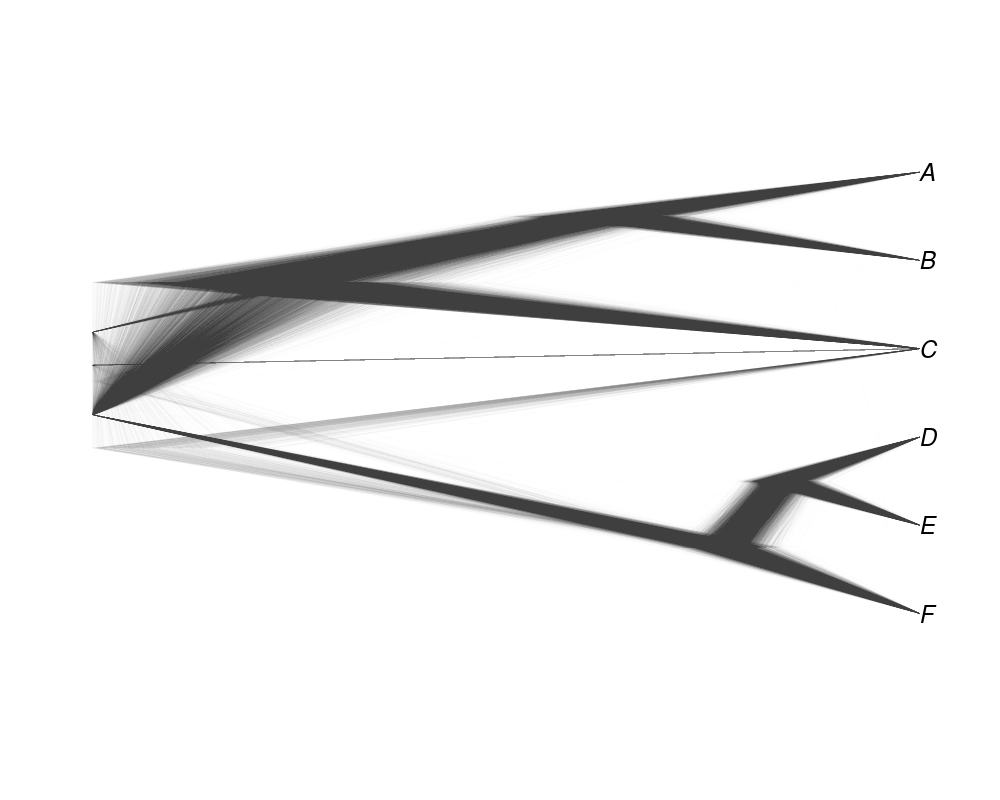
\includegraphics[height=0.2\textheight]{example_3/twin_posterior_gen.png}
    };   
    \node[state] (DT) [below of = CT, rectangle] {
      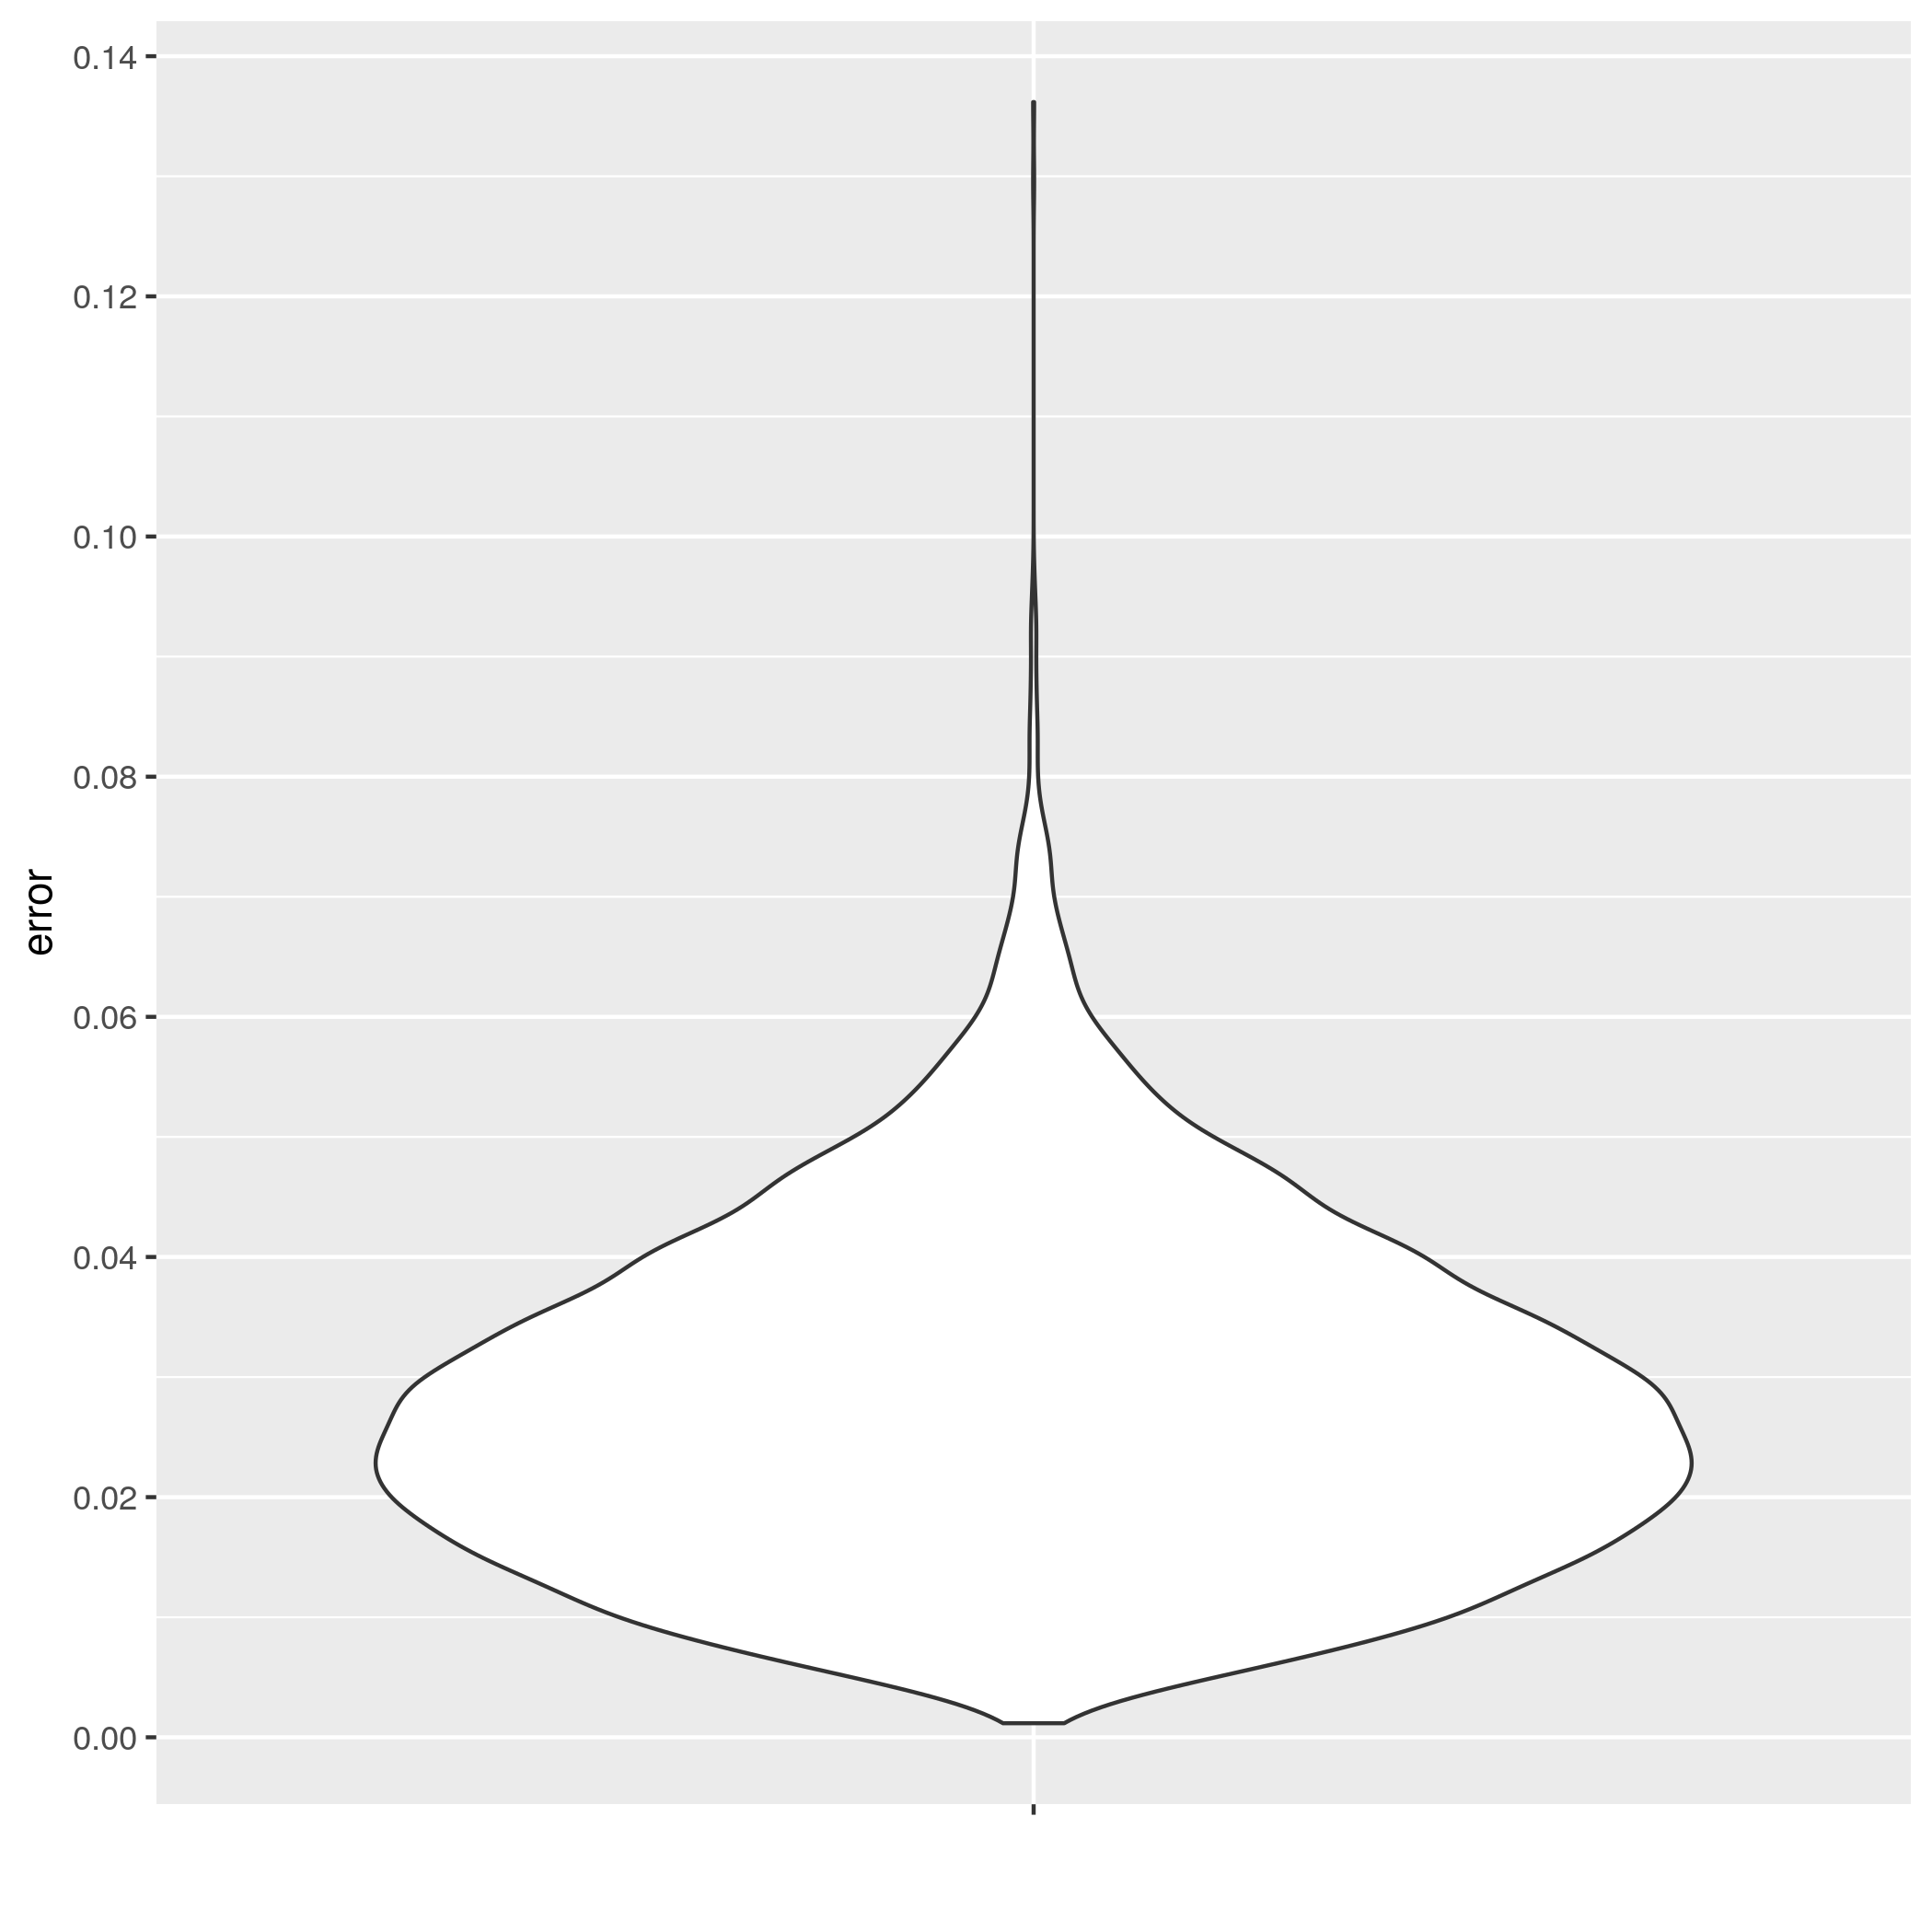
\includegraphics[height=0.2\textheight]{example_3/twin_error_violin_gen.png}
    };   
    \path 
      (O) edge [anchor = south] node {} (A)
      (A) edge [anchor = south] node {} (B)
      (B) edge [anchor = south] node {} (C)
      (C) edge [anchor = south] node {} (D)
      (A) edge [anchor = east] node {} (AT)
      (AT) edge [anchor = south] node {} (BT)
      (BT) edge [anchor = south] node {} (CT)
      (CT) edge [anchor = south] node {} (DT)
    ; 
    \end{tikzpicture}
  }
  \label{fig:example_3_full_pipeline}
  \caption{Example 3: full pipeline}
\end{figure}
%%%%%%%%%%%%%%%%%%%%%%%%%%%%%%%%%%%%%%%%%%%%%%%%%%%%%%%%%%%%%%%%%%%%%%%%%%%%%%%%

\input{example_3/esses.latex}
% has label tab:esses_example_3

%%%%%%%%%%%%%%%%%%%%%%%%%%%%%%%%%%%%%%%%%%%%%%%%%%%%%%%%%%%%%%%%%%%%%%%%%%%%%%%%
\subsection{Example 4}
%%%%%%%%%%%%%%%%%%%%%%%%%%%%%%%%%%%%%%%%%%%%%%%%%%%%%%%%%%%%%%%%%%%%%%%%%%%%%%%%

%%%%%%%%%%%%%%%%%%%%%%%%%%%%%%%%%%%%%%%%%%%%%%%%%%%%%%%%%%%%%%%%%%%%%%%%%%%%%%%%
\begin{figure}[ht]
  \centering
  \resizebox {1.0\columnwidth} {!} {
    \begin{tikzpicture}[
      ->,>=stealth',shorten >=1pt,auto,
      node distance=0.5\textheight, 
      semithick
    ]   
    \tikzstyle{every state}=[]
    \node[state, draw=none] (O) [] {
    };   
    \node[state] (A) [right of = O, rectangle] {
      \includegraphics[height=0.4\textheight]{example_4/true_tree.png}
    };   
    \node[state] (B) [below of = A, rectangle] {
      \includegraphics[height=0.45\textheight]{example_4/true_alignment.png}
    };   
    \node[state] (CB) [below of = B, rectangle, node distance=0.8\textheight] {
      
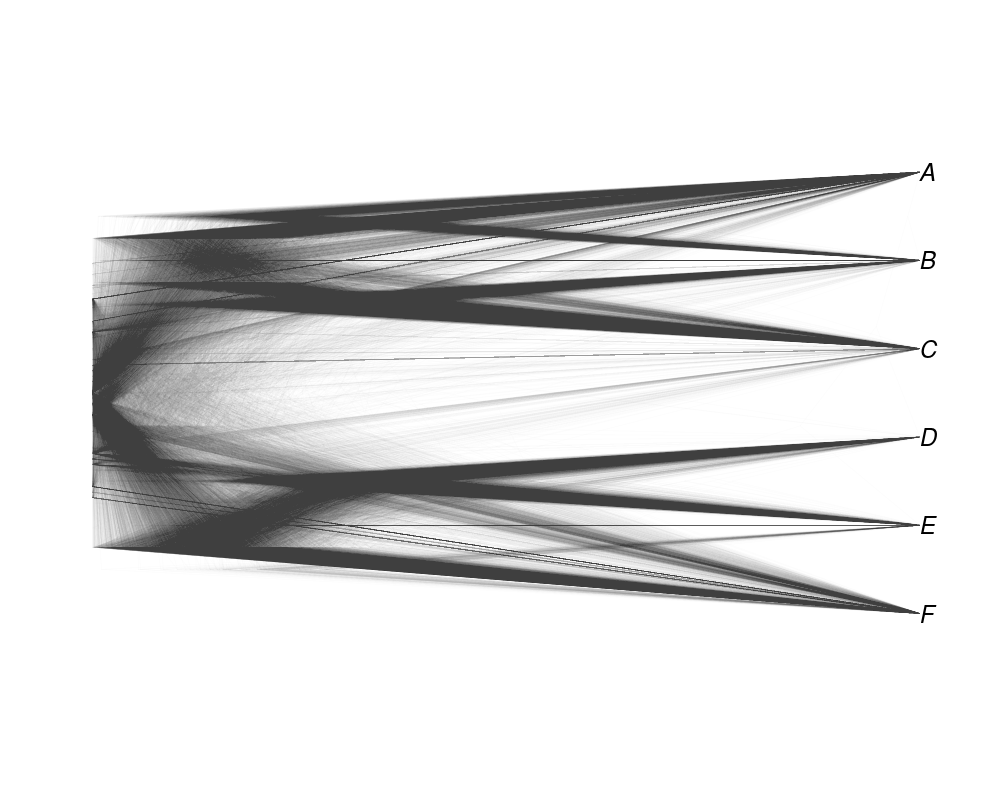
\includegraphics[height=0.95\textheight]{example_4/true_posterior_best.png}
    };   
    \node[state] (DB) [below of = CB, rectangle, node distance=1.0\textheight] {
      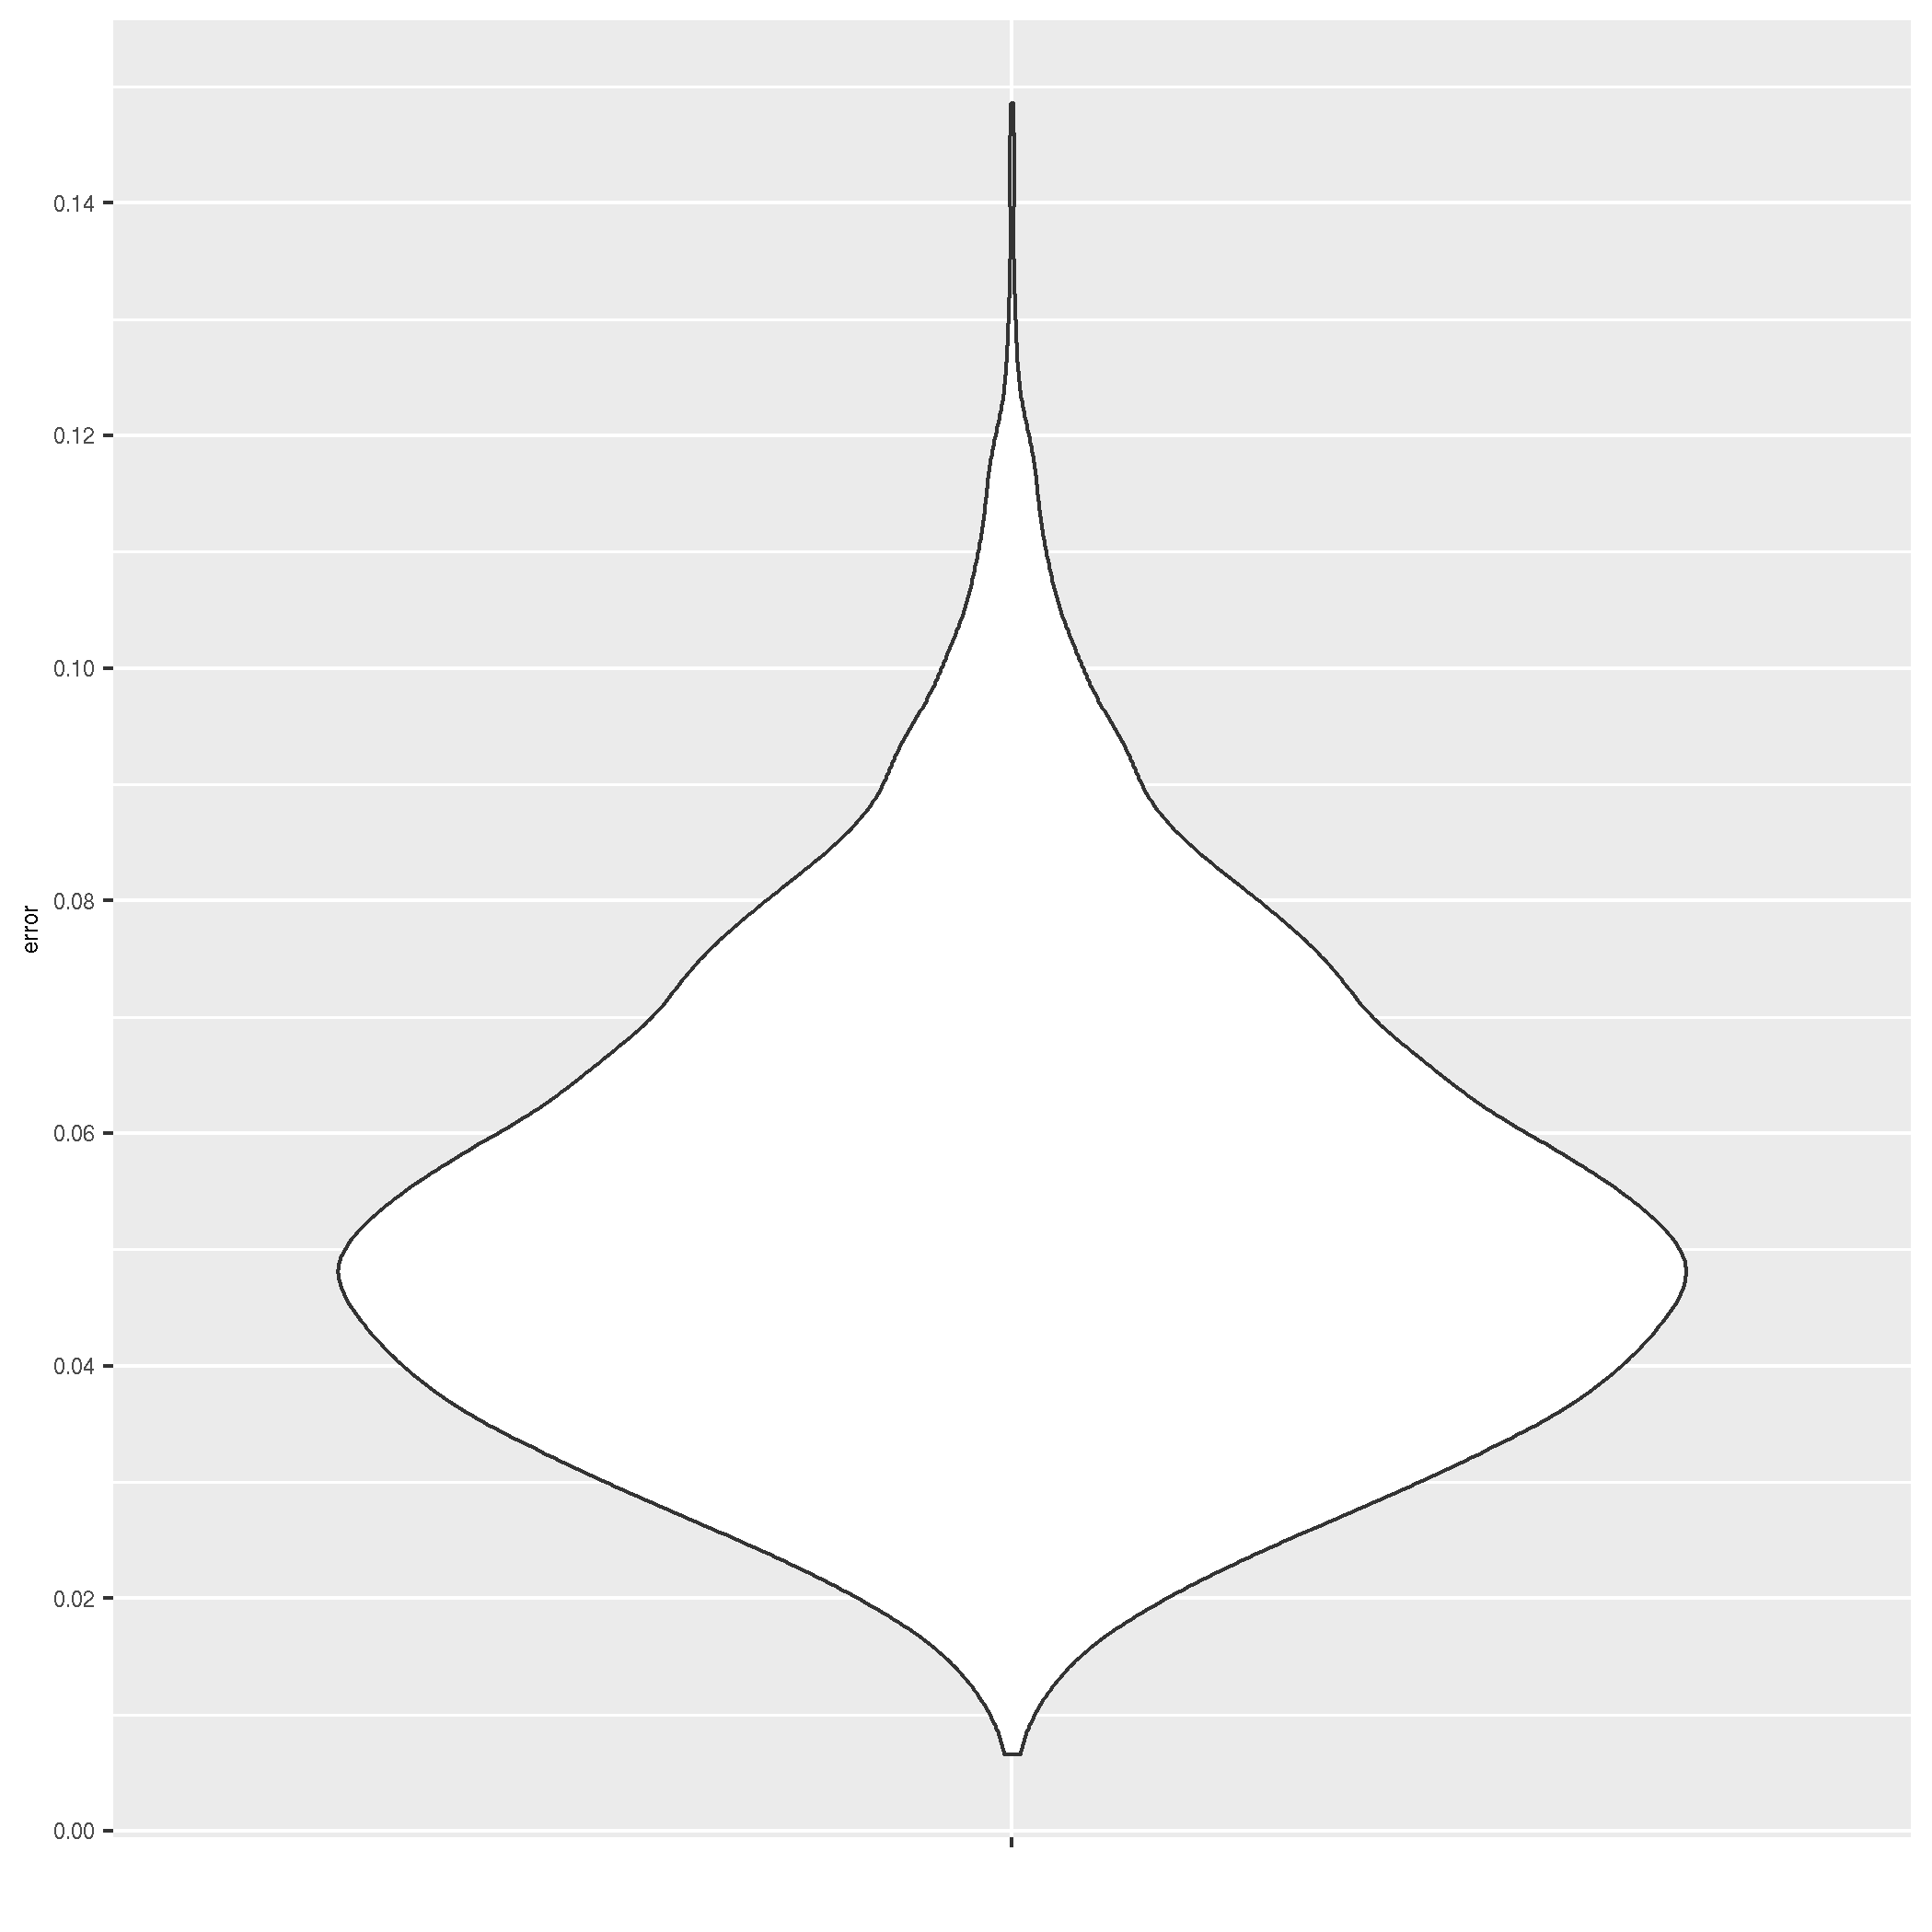
\includegraphics[height=0.65\textheight]{example_4/true_error_violin_best.png}
    };   
    \node[state] (AT) [right of = A, rectangle, node distance=2.0\textwidth] {
      \includegraphics[height=0.4\textheight]{example_4/twin_tree.png}
    };   
    \node[state] (BT) [below of = AT, rectangle] {
      \includegraphics[height=0.45\textheight]{example_4/twin_alignment.png}
    };   
    \node[state] (CTB) [below of = BT, rectangle, node distance=0.8\textheight] 
{
      
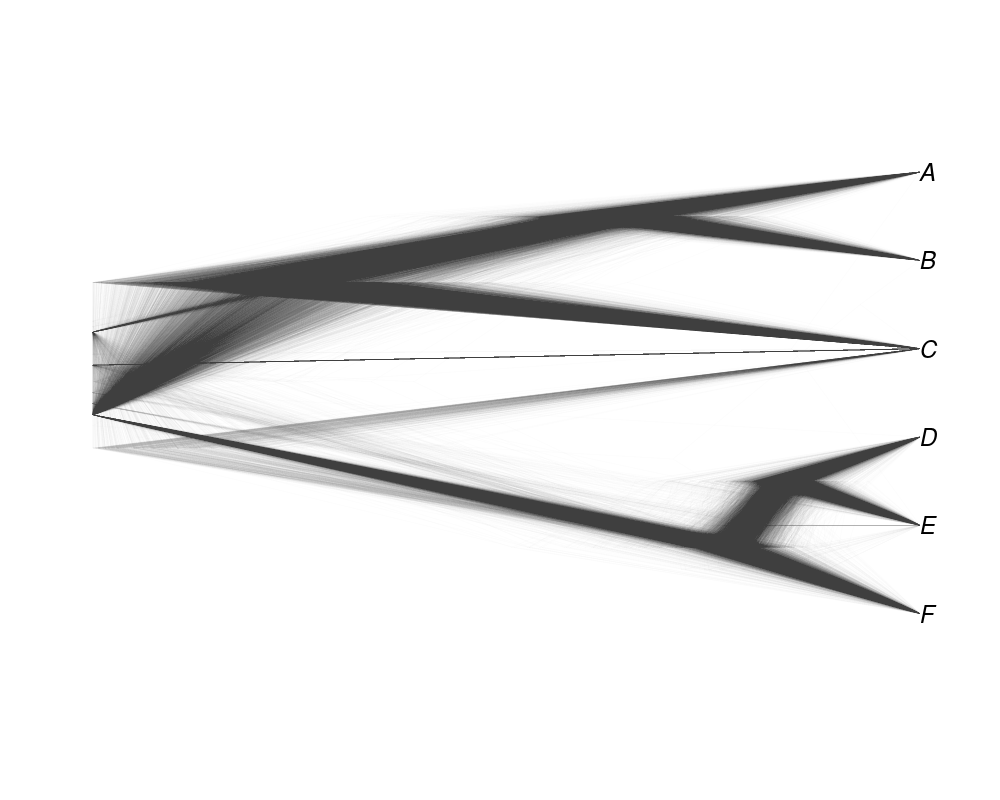
\includegraphics[height=0.95\textheight]{example_4/twin_posterior_best.png}
    };   
    \node[state] (DTB) [below of = CTB, rectangle, node 
distance=1.0\textheight] {
      
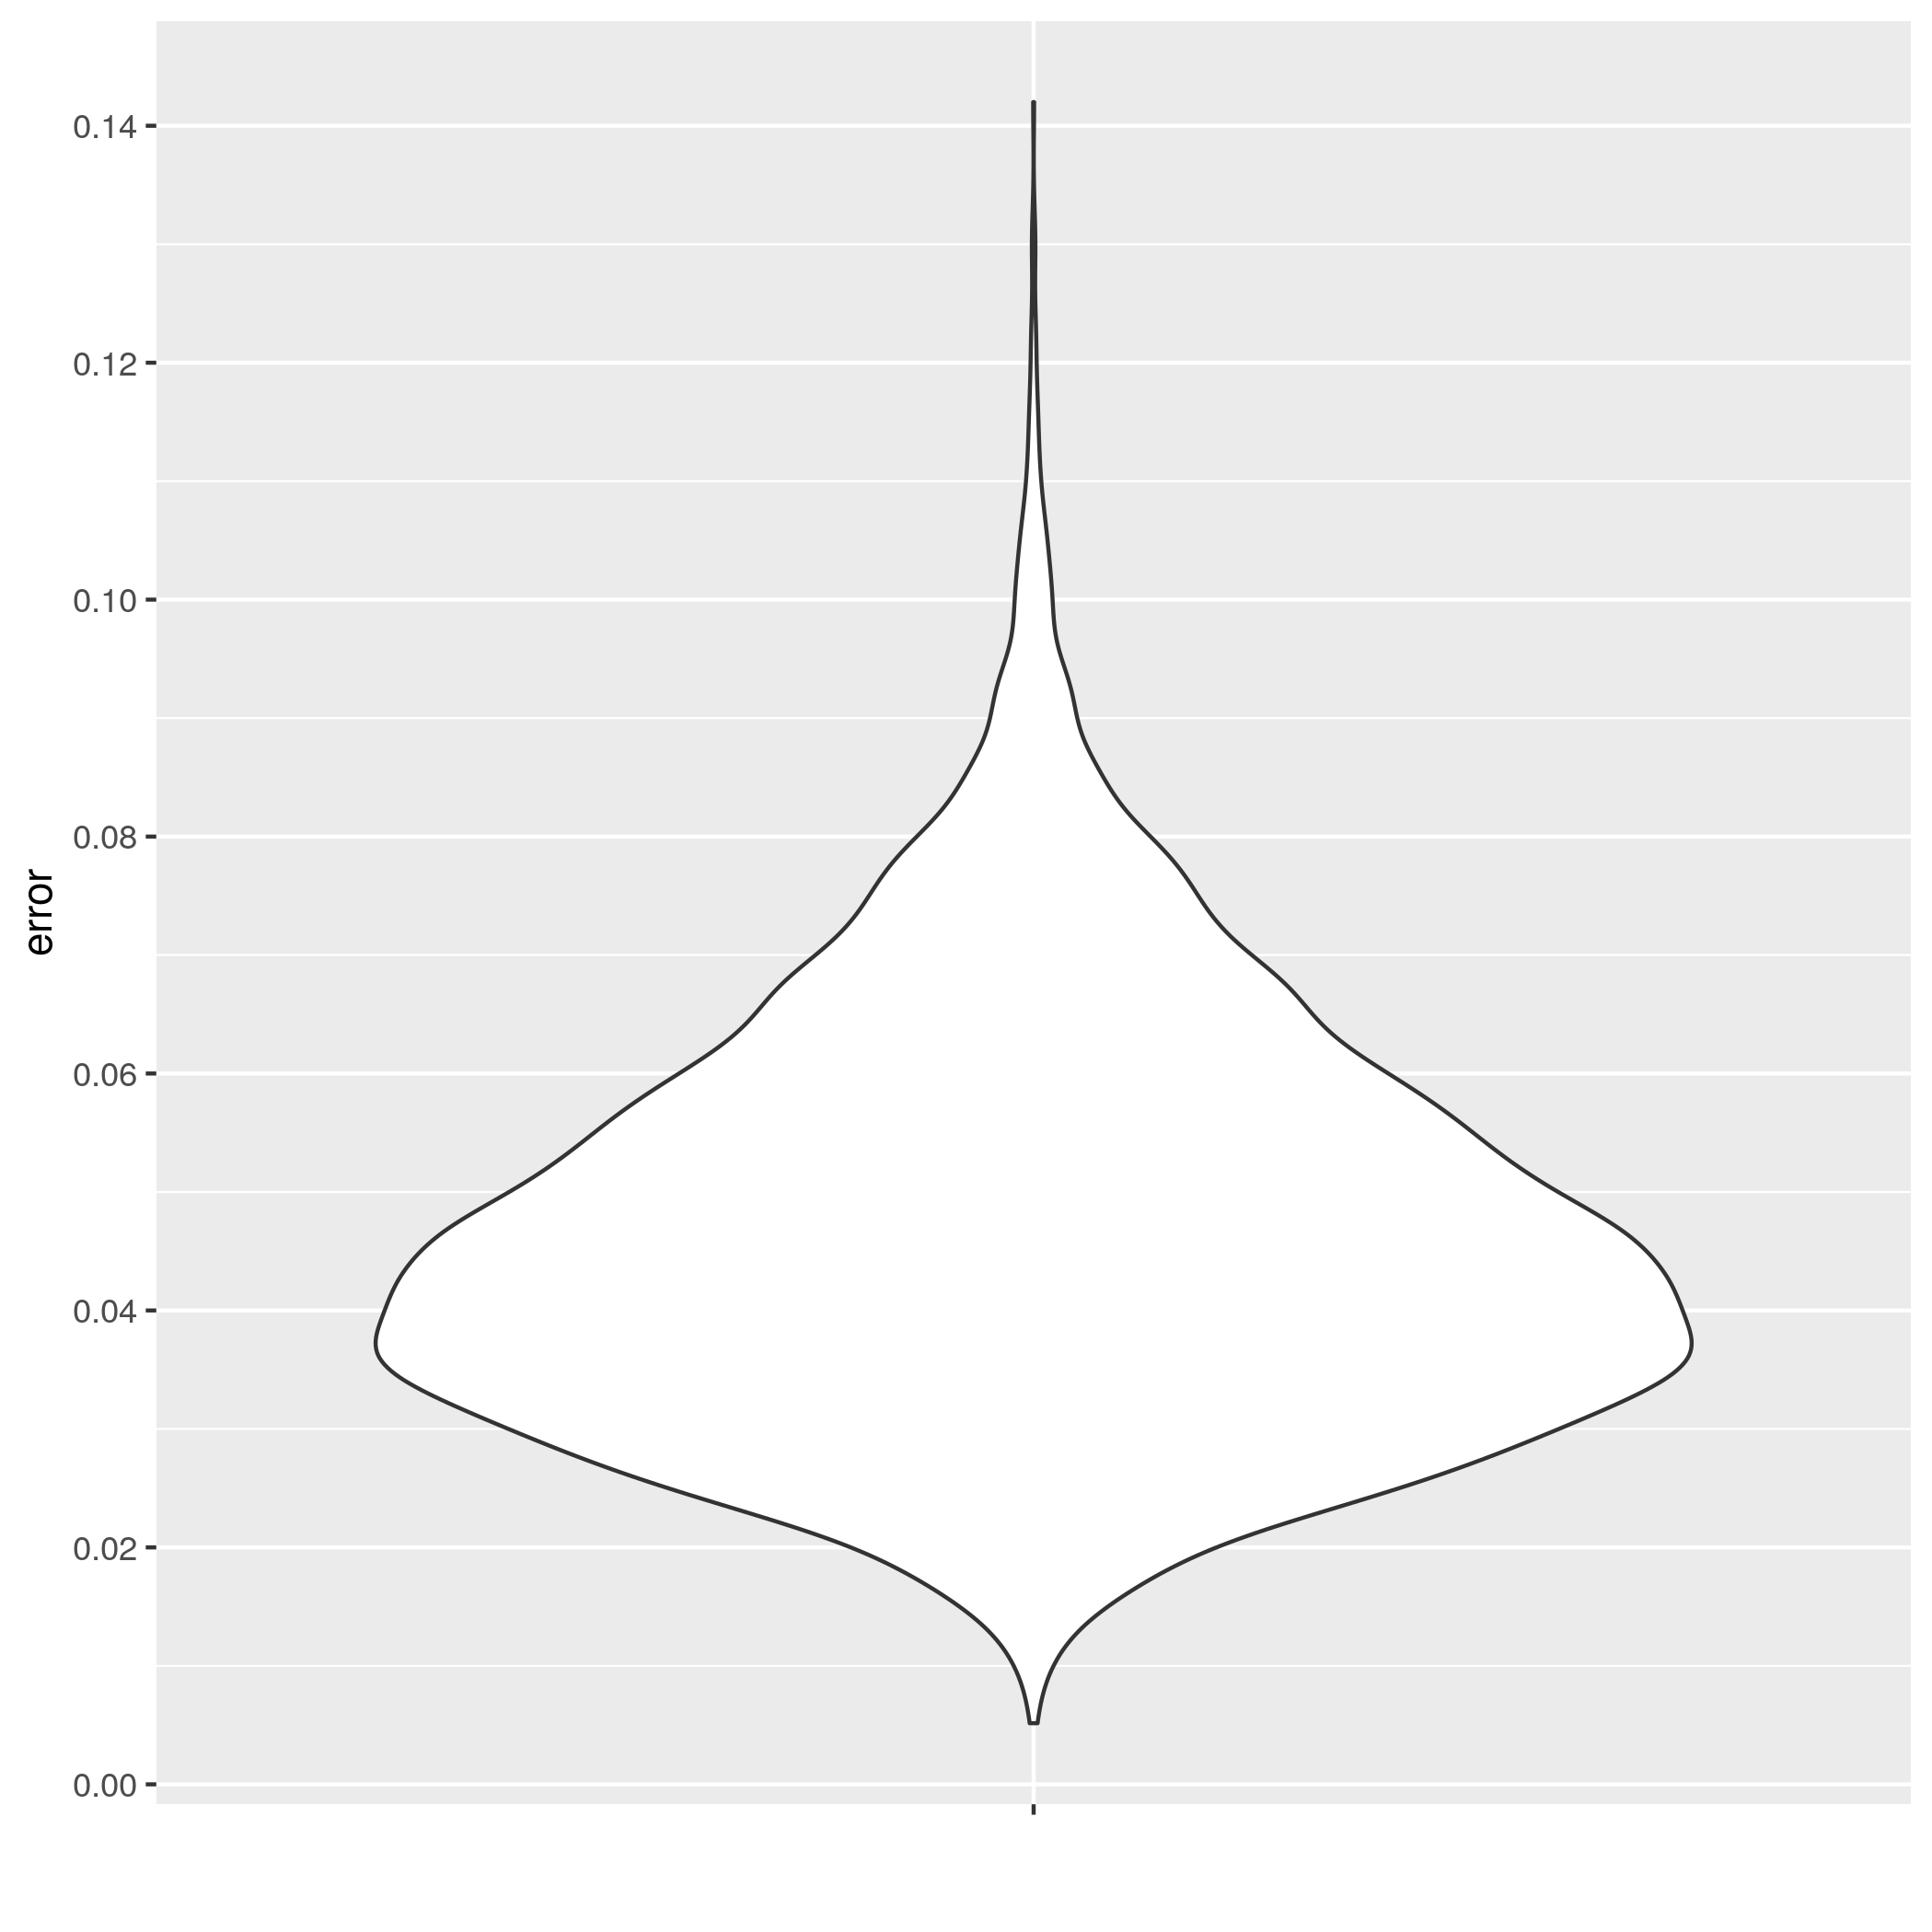
\includegraphics[height=0.65\textheight]{example_4/twin_error_violin_best.png}
    };   
    \path 
      (O) edge [anchor = south] node {} (A)
      (A) edge [anchor = south] node {} (B)
      (B) edge [anchor = south east] node {} (CB)
      (CB) edge [anchor = south] node {} (DB)
      (A) edge [anchor = east] node {} (AT)
      (AT) edge [anchor = south] node {} (BT)
      (BT) edge [anchor = south] node {} (CTB)
      (CTB) edge [anchor = south] node {} (DTB)
    ; 
    \end{tikzpicture}
  }
  \label{fig:example_4_full_pipeline}
  \caption{Example 4: full pipeline}
\end{figure}
%%%%%%%%%%%%%%%%%%%%%%%%%%%%%%%%%%%%%%%%%%%%%%%%%%%%%%%%%%%%%%%%%%%%%%%%%%%%%%%%


\input{example_4/esses_best.latex}
% has label tab:esses_example_4_best

\input{example_4/esses_twin_best.latex}
% has label tab:esses_example_4_twin_best

\input{example_4/evidence_true.latex}
% has label tab:evidences_example_4

\input{example_4/evidence_twin.latex}
% has label tab:evidences_example_4

%%%%%%%%%%%%%%%%%%%%%%%%%%%%%%%%%%%%%%%%%%%%%%%%%%%%%%%%%%%%%%%%%%%%%%%%%%%%%%%%
\subsection{Example 5}
%%%%%%%%%%%%%%%%%%%%%%%%%%%%%%%%%%%%%%%%%%%%%%%%%%%%%%%%%%%%%%%%%%%%%%%%%%%%%%%%

%%%%%%%%%%%%%%%%%%%%%%%%%%%%%%%%%%%%%%%%%%%%%%%%%%%%%%%%%%%%%%%%%%%%%%%%%%%%%%%%
\begin{figure}[ht]
  \centering
  \resizebox {0.8\columnwidth} {!} {
    \begin{tikzpicture}[
      ->,>=stealth',shorten >=1pt,auto,
      node distance=0.4\textheight, 
      semithick
    ]   
    \tikzstyle{every state}=[]
    \node[state, draw=none] (O) [] {
    };   
    \node[state] (A) [right of = O, rectangle] {
      \includegraphics[height=0.2\textheight]{example_5/true_tree.png}
    };   
    \node[state] (B) [below of = A, rectangle] {
      \includegraphics[height=0.13\textheight]{example_5/true_alignment.png}
    };   
    \node[state] (CG) [below of = B, rectangle] {
      
\includegraphics[height=0.2\textheight]{example_5/true_posterior_gen.png}
    };   
    \node[state] (DG) [below of = CG, rectangle] {
      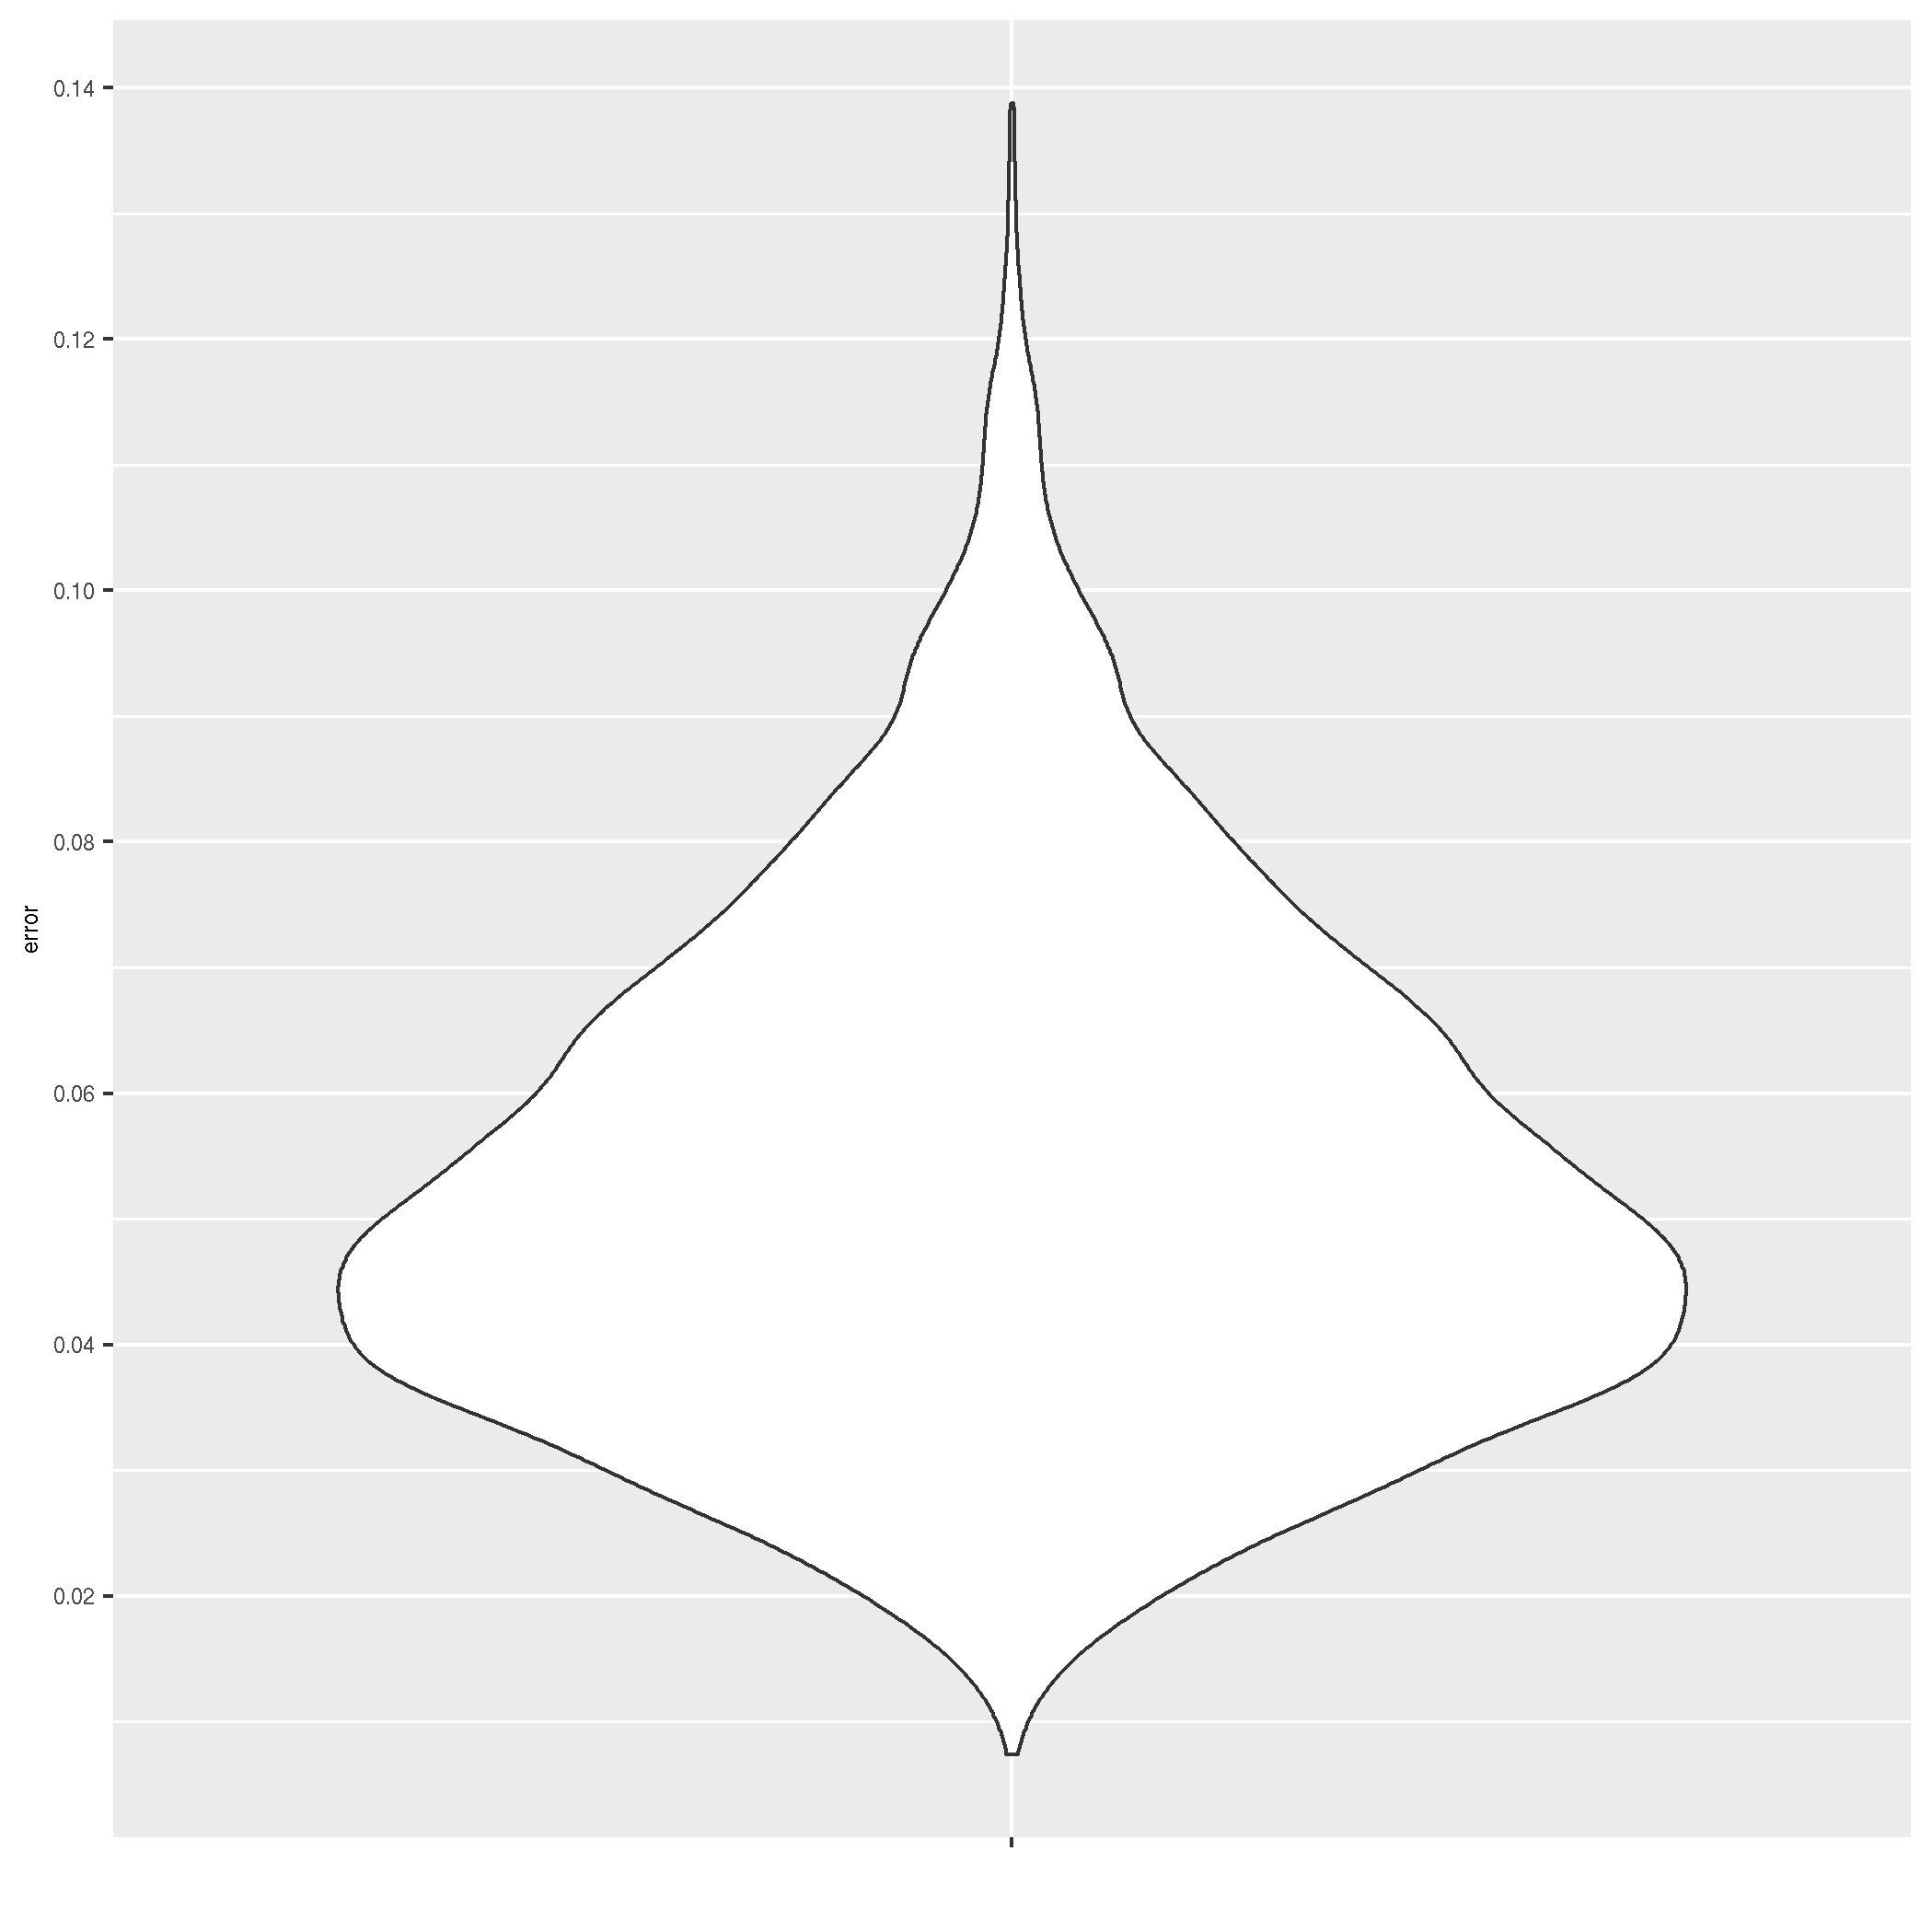
\includegraphics[height=0.2\textheight]{example_5/true_error_violin_gen.png}
    };   
    \node[state] (CB) [right of = C, rectangle] {
      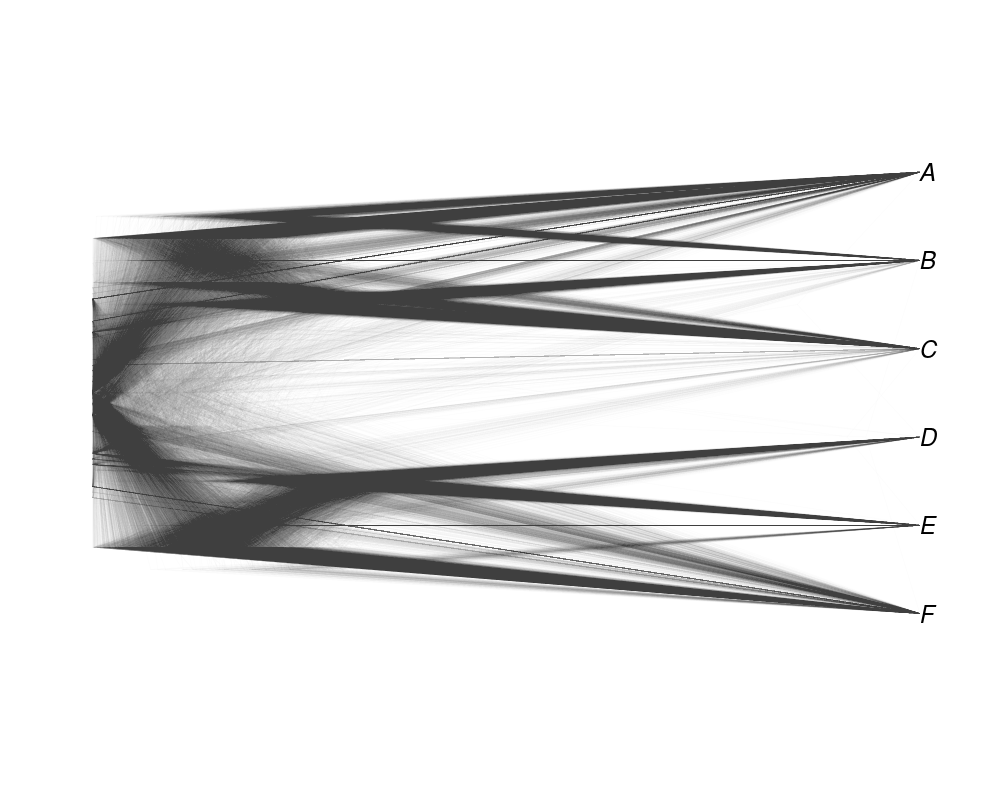
\includegraphics[height=0.2\textheight]{example_5/true_posterior_best.png}
    };   
    \node[state] (DB) [below of = CB, rectangle] {
      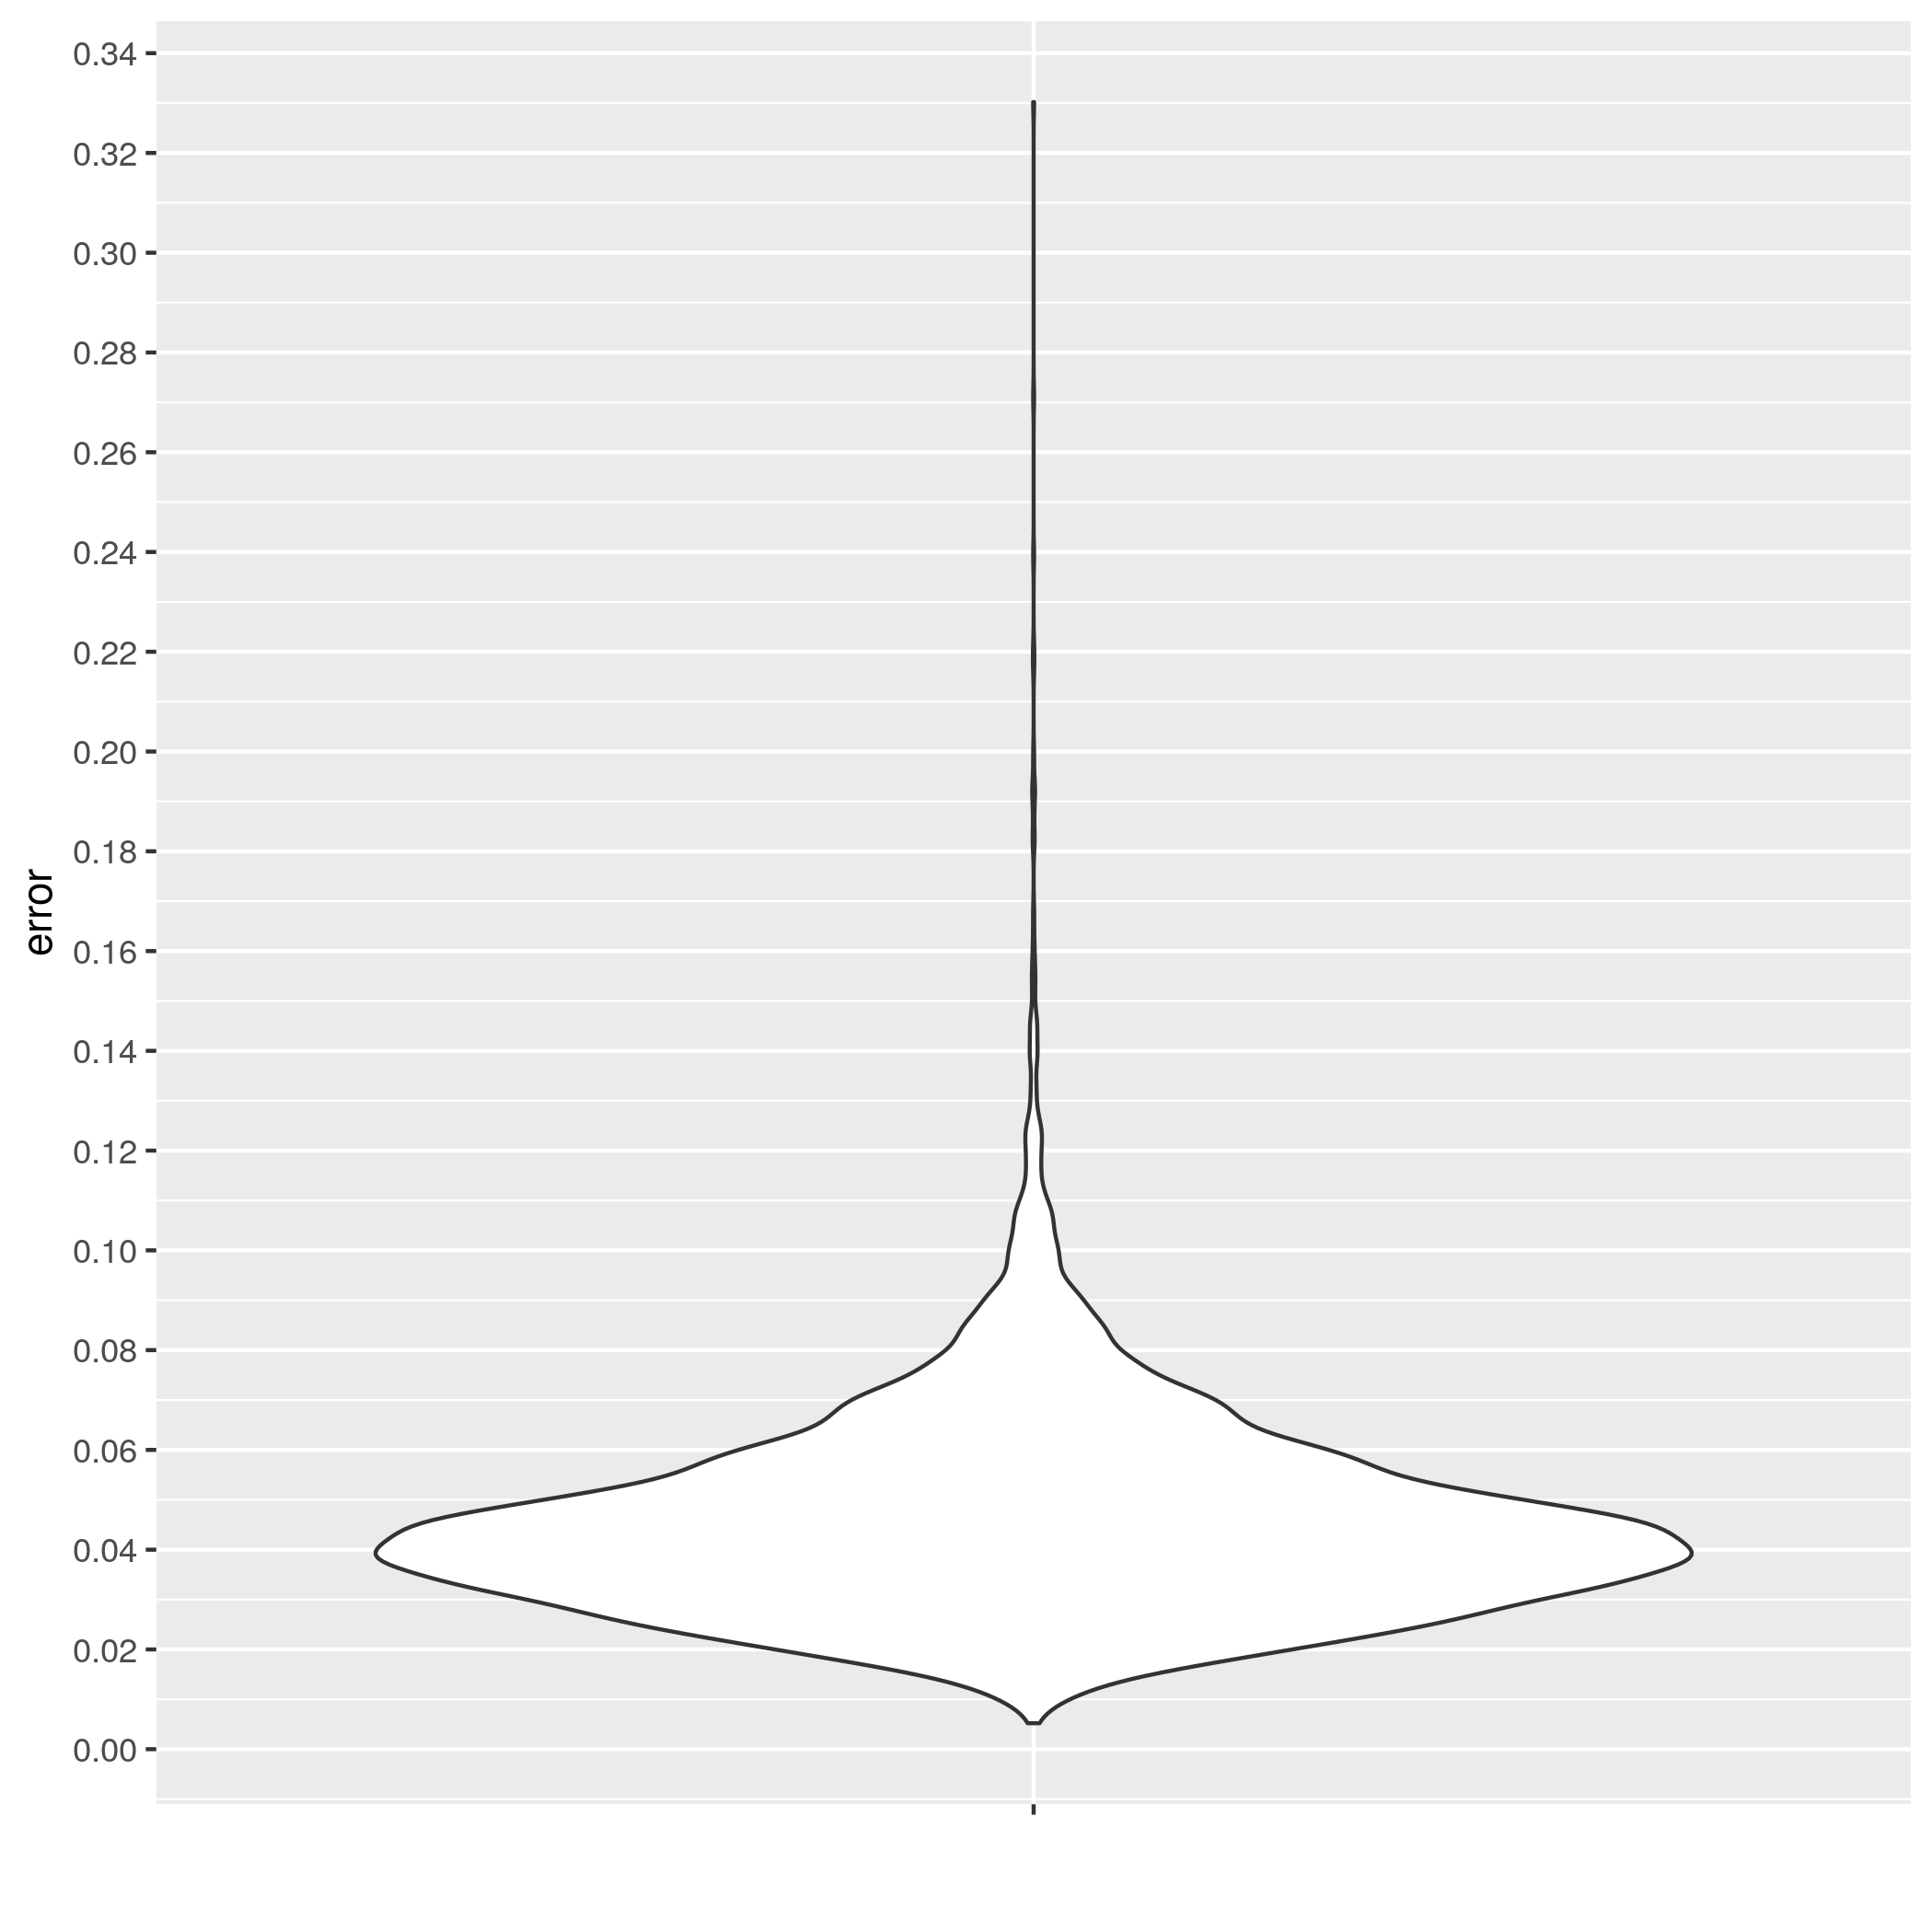
\includegraphics[height=0.2\textheight]{example_5/true_error_violin_best.png}
    };   
    \node[state] (AT) [right of = A, rectangle, node distance=0.8\textheight] {
      \includegraphics[height=0.2\textheight]{example_5/twin_tree.png}
    };   
    \node[state] (BT) [below of = AT, rectangle] {
      \includegraphics[height=0.13\textheight]{example_5/twin_alignment.png}
    };   
    \node[state] (CTG) [below of = BT, rectangle] {
      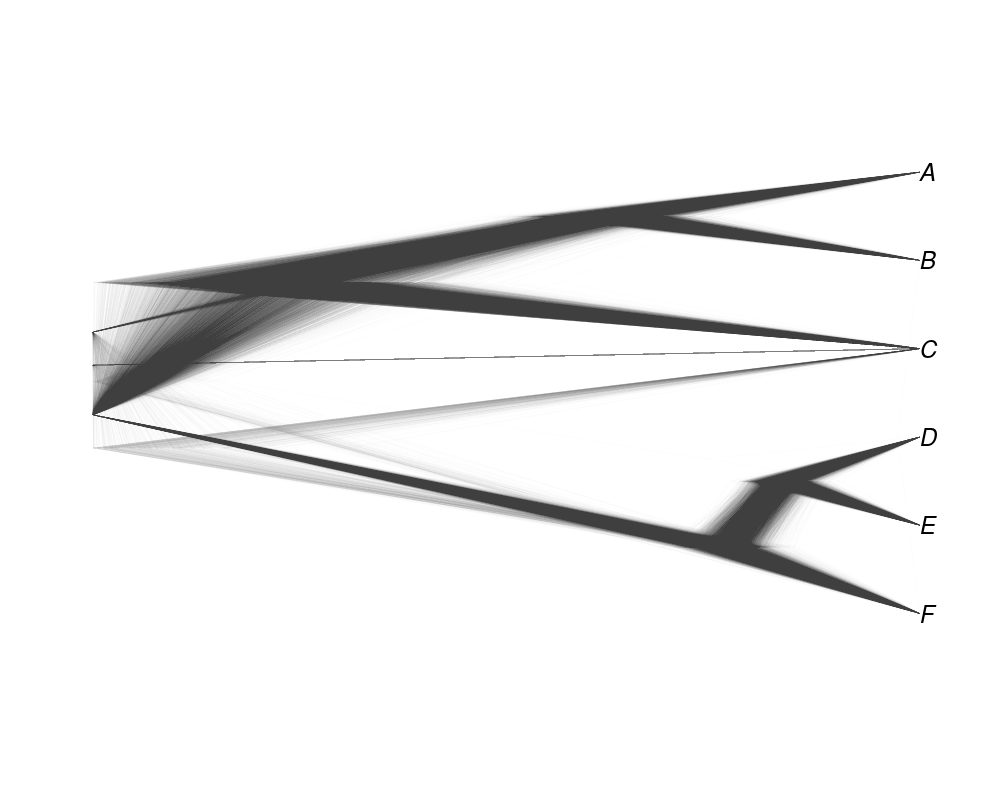
\includegraphics[height=0.2\textheight]{example_5/twin_posterior_gen.png}
    };   
    \node[state] (DTG) [below of = CTG, rectangle] {
      
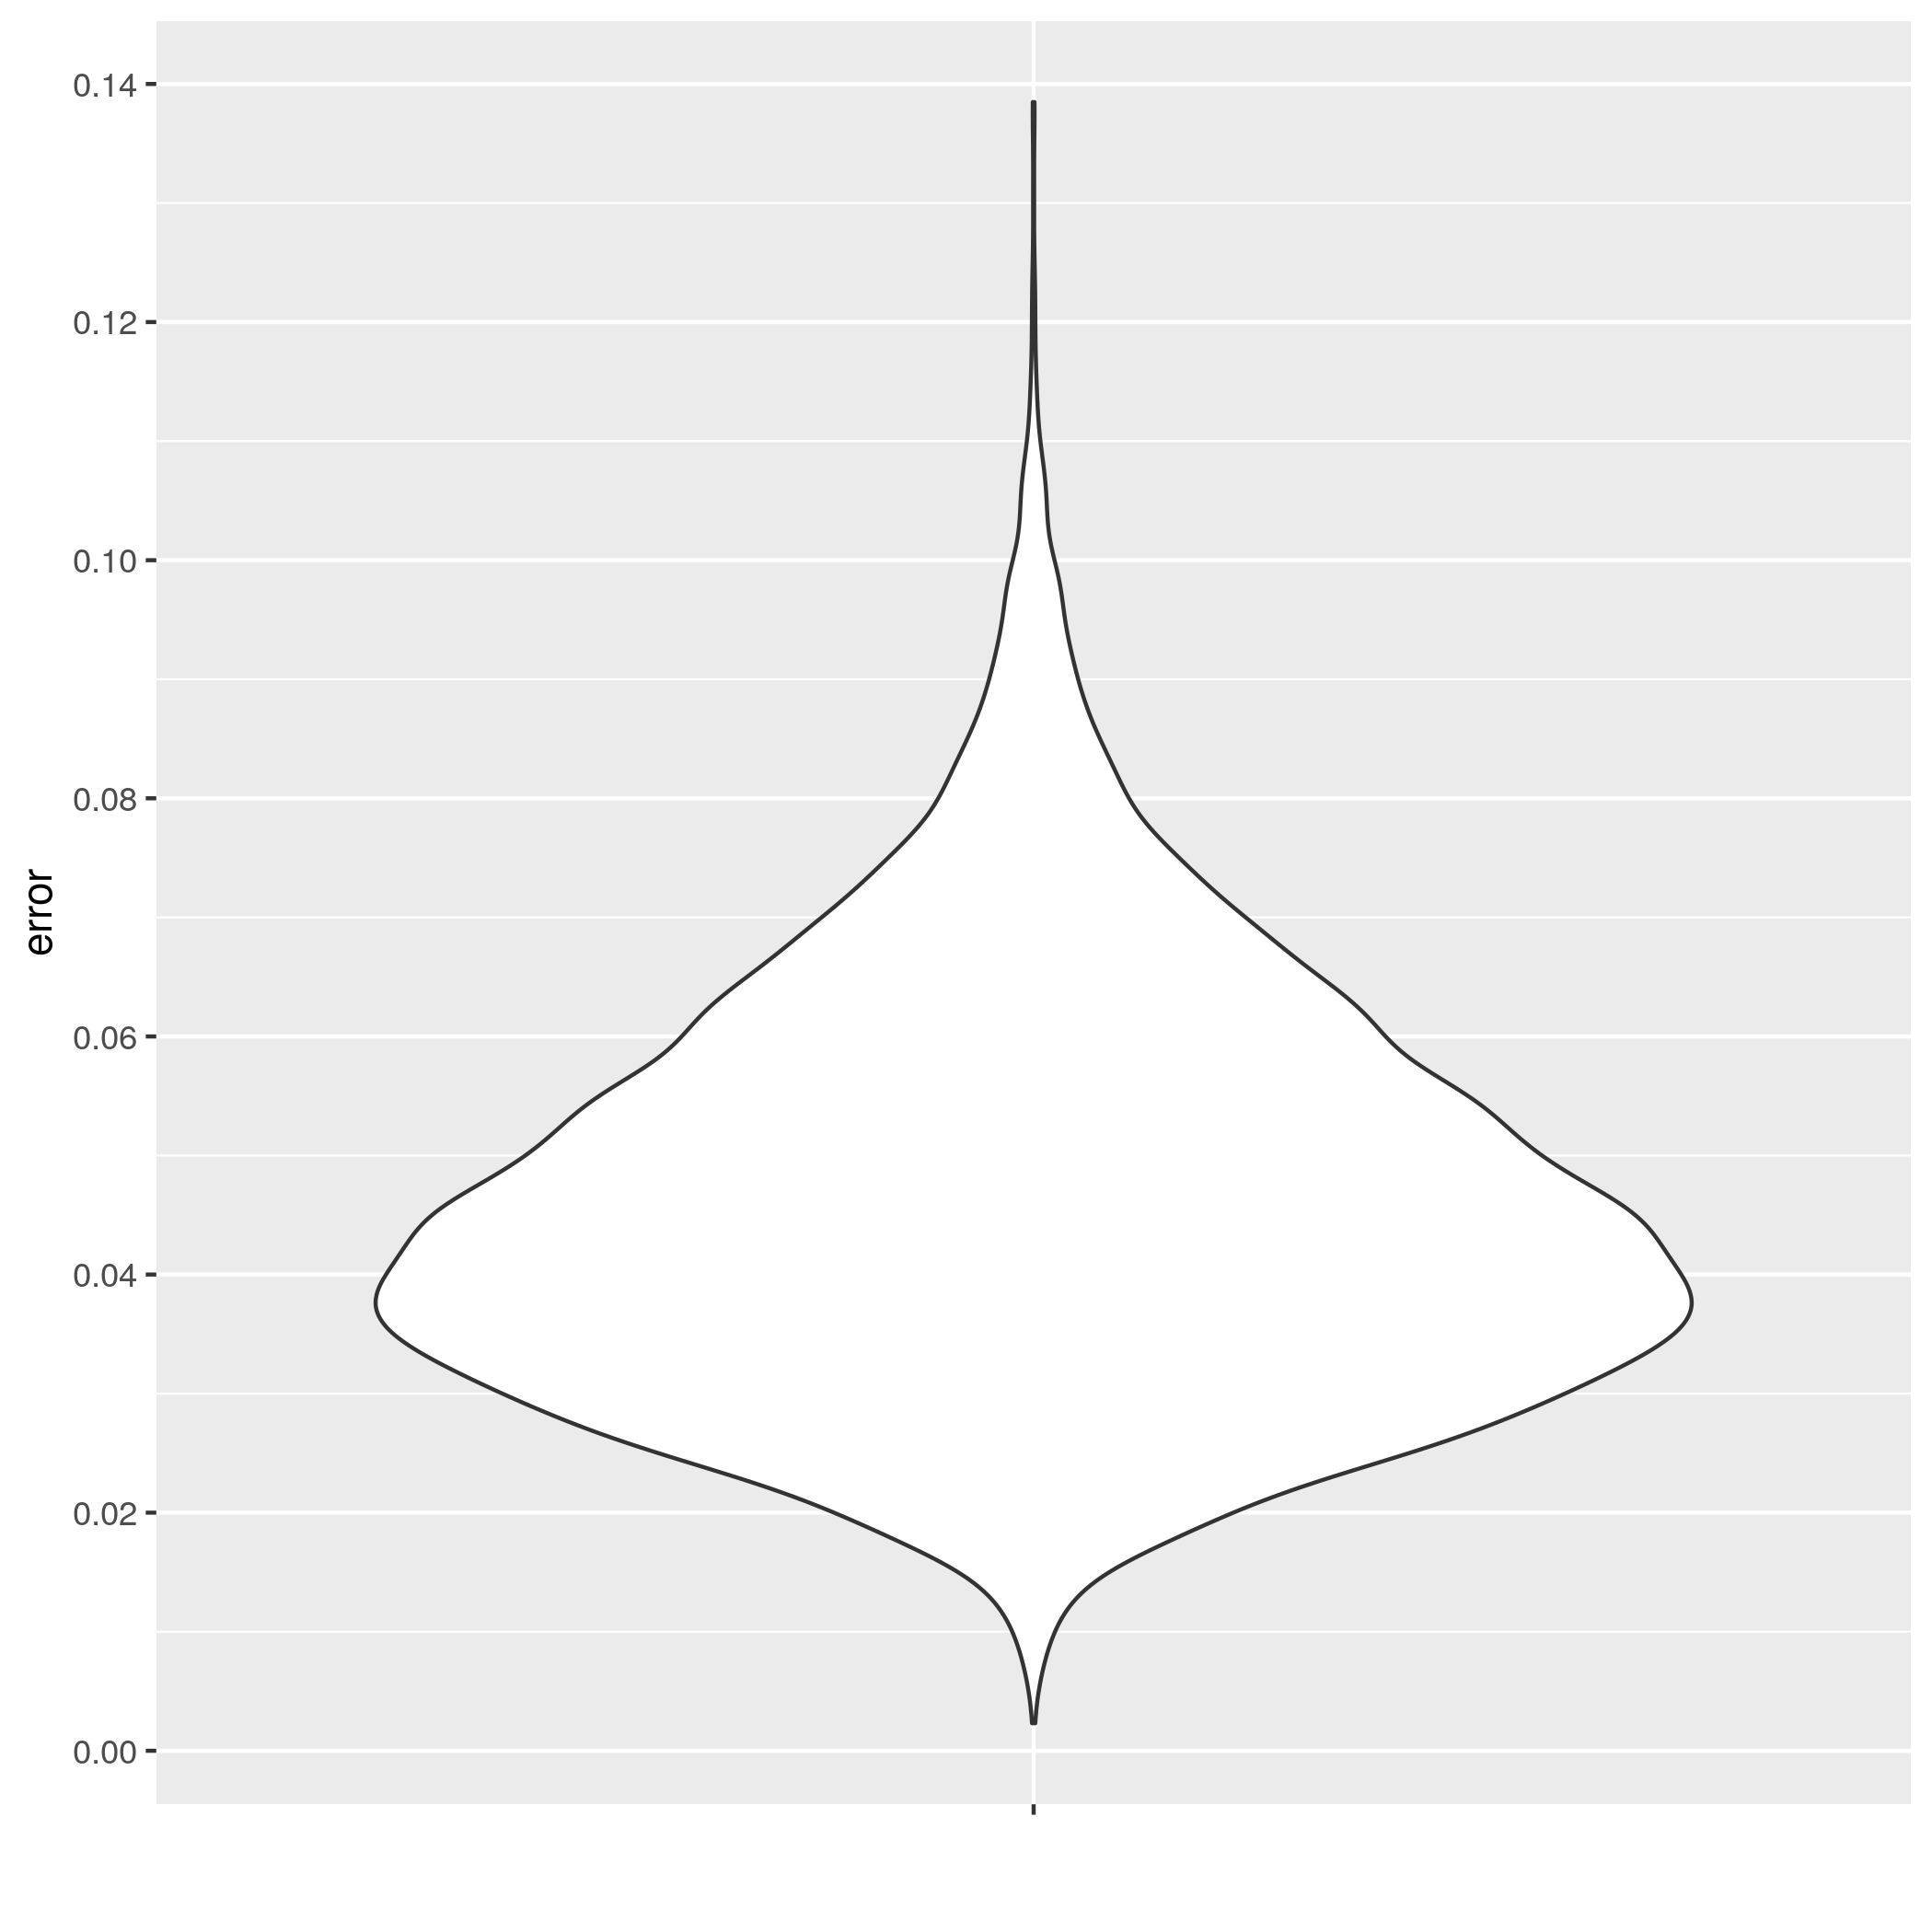
\includegraphics[height=0.2\textheight]{example_5/twin_error_violin_gen.png}
    };   
    \node[state] (CTB) [right of = CTG, rectangle] {
      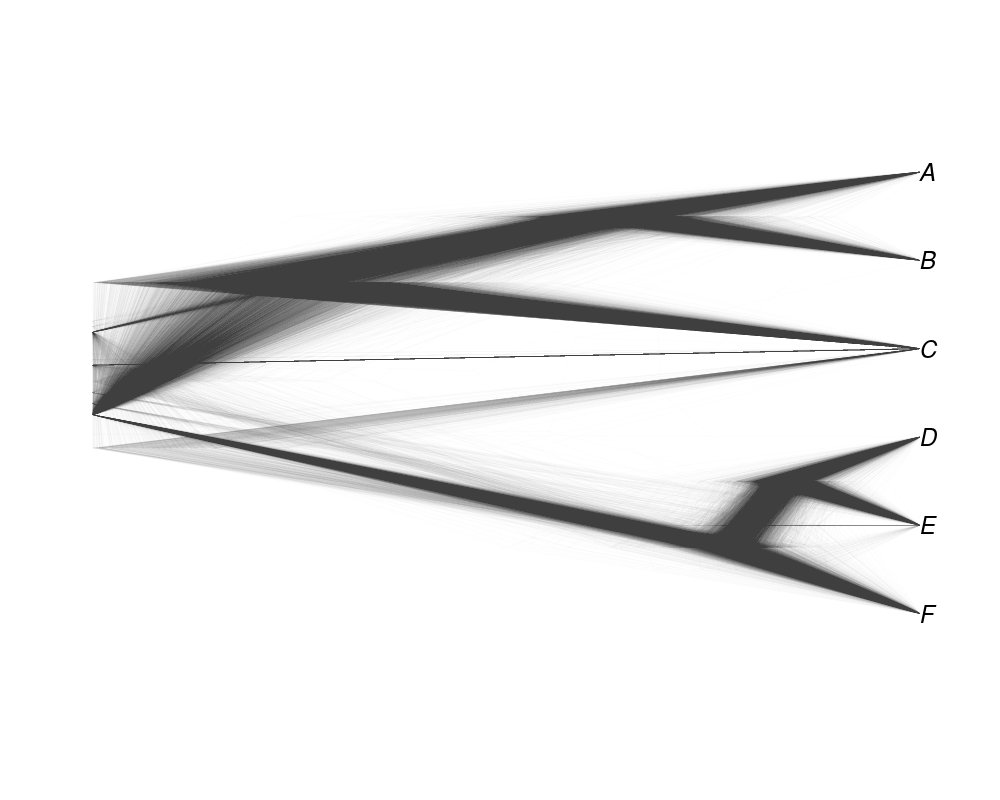
\includegraphics[height=0.2\textheight]{example_5/twin_posterior_best.png}
    };   
    \node[state] (DTB) [below of = CTB, rectangle] {
      
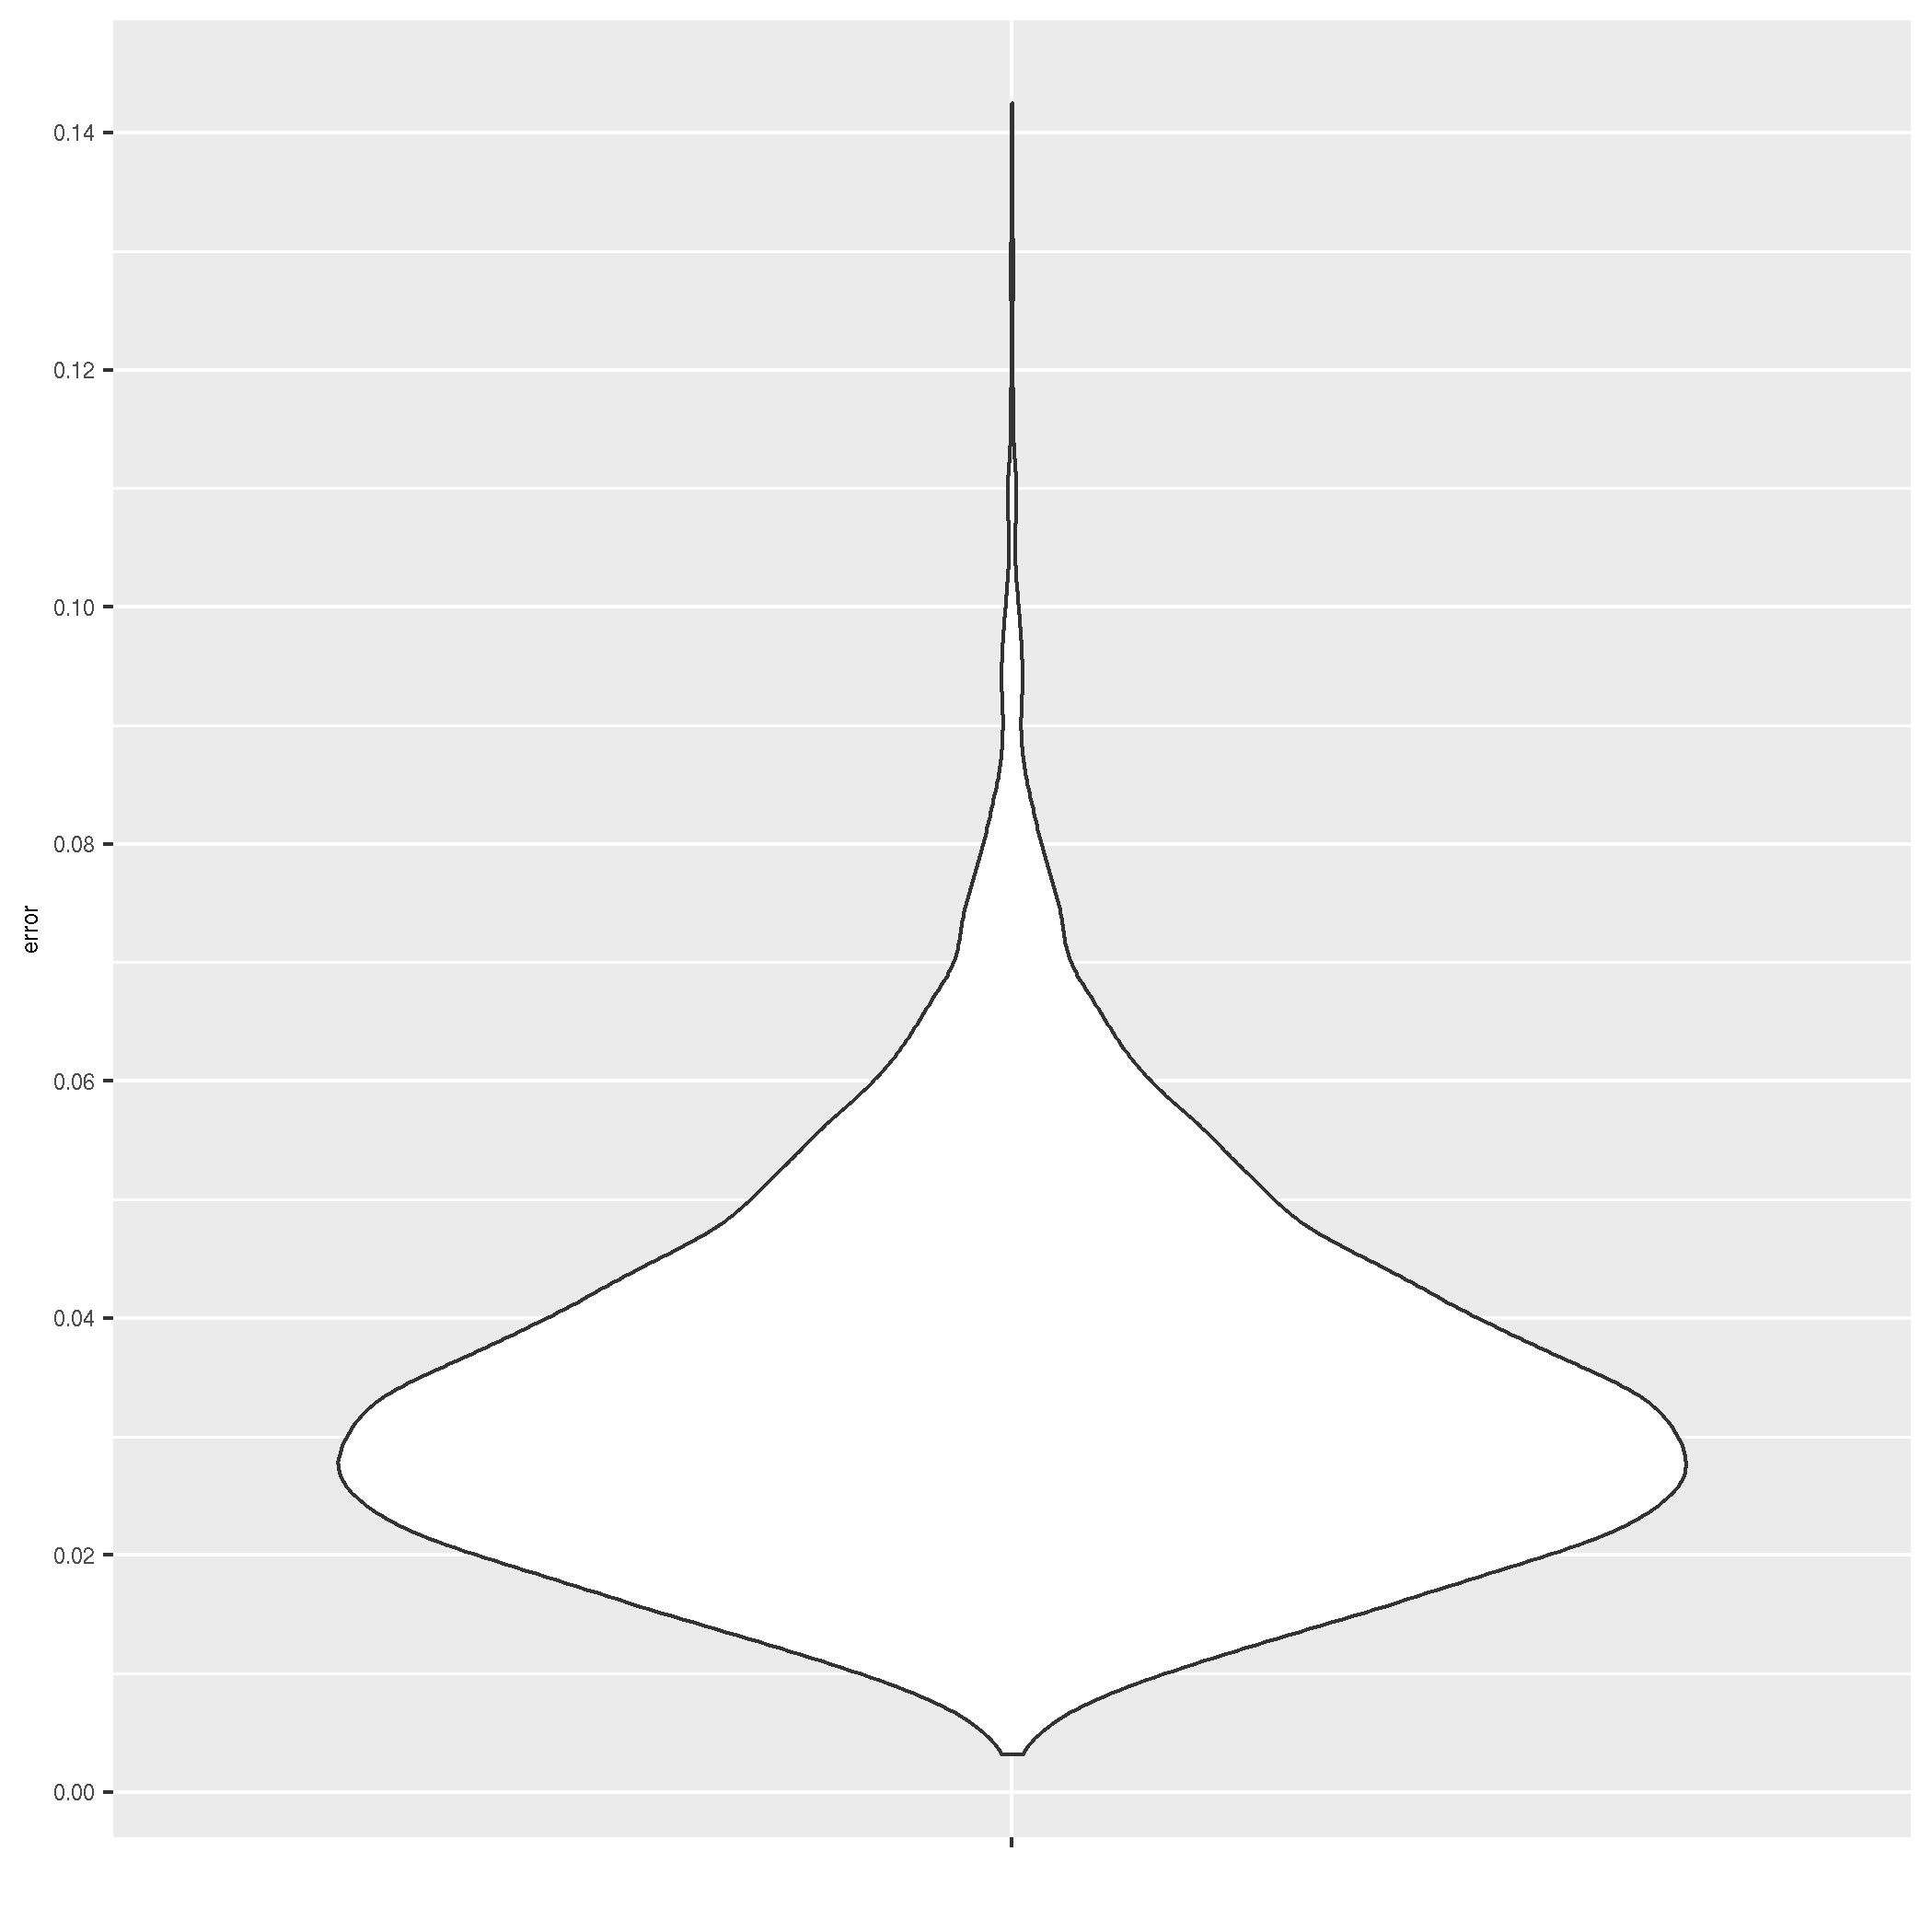
\includegraphics[height=0.2\textheight]{example_5/twin_error_violin_best.png}
    };   
    \path 
      (O) edge [anchor = south] node {} (A)
      (A) edge [anchor = south] node {} (B)
      (B) edge [anchor = south] node {} (CG)
      (CG) edge [anchor = south] node {} (DG)
      (B) edge [anchor = south east] node {} (CB)
      (CB) edge [anchor = south] node {} (DB)
      (A) edge [anchor = east] node {} (AT)
      (AT) edge [anchor = south] node {} (BT)
      (BT) edge [anchor = south east] node {} (CTG)
      (CTG) edge [anchor = south] node {} (DTG)
      (BT) edge [anchor = south] node {} (CTB)
      (CTB) edge [anchor = south] node {} (DTB)
    ; 
    \end{tikzpicture}
  }
  \label{fig:example_5_full_pipeline}
  \caption{Example 5: full pipeline}
\end{figure}
%%%%%%%%%%%%%%%%%%%%%%%%%%%%%%%%%%%%%%%%%%%%%%%%%%%%%%%%%%%%%%%%%%%%%%%%%%%%%%%%

\input{example_5/esses_gen.latex}
% has label tab:esses_example_5_gen

\input{example_5/esses_best.latex}
% has label tab:esses_example_5_best

\input{example_5/esses_twin_gen.latex}
% has label tab:esses_example_5_twin_gen

\input{example_5/esses_twin_best.latex}
% has label tab:esses_example_5_twin_best

\input{example_5/evidence_true.latex}
% has label tab:evidences_example_5

\input{example_5/evidence_twin.latex}
% has label tab:evidences_example_5

\end{document}
